\documentclass[12pt,english]{article}

\input{fragment/preamble_package}
% Citation comes loading other packages, so that footnotes follow biblatex-chicago style
\input{fragment/preamble_citation}

% Responses to Referees
\usepackage{blindtext}
\newcommand{\aptxspc}{1.8}
\newcommand{\rrquote}{1.1}
\newcommand{\rrxspc}{1.5}

\begin{document}
% Allow modest extra interword stretch to avoid overfull lines from unbreakable
% content (URLs, email addresses, LARGE cover lines).
\emergencystretch=3em

% % SUBMISSION COVER
% \thispagestyle{empty}
% \begingroup
%   \doublespacing
%   \centering
%   \LARGE \PAPERTITLE
% \endgroup
% This document contains the submission version of the manuscript ``More Residents, Better Care? Evidence from Medicaid Expansion'' for [JOURNAL NAME]. It includes:
% \begin{enumerate}
%     \item Title page information
%     \begin{itemize}
%         \item Title and Author
%         \item Abstract
%         \item Keywords
%         \item Acknowledgment
%     \end{itemize}
%     \item The manuscript
%     \begin{itemize}
%         \item Main manuscript text
%         \item Main manuscript references
%         \item Main manuscript figures
%         \item Main manuscript tables
%     \end{itemize}  
%     \item The online appendix, which is separately paged. It includes an online appendix title page, appendices A (tables) and B (figures), and references for citations in the appendix.
% \end{enumerate}
\clearpage


%%%%%%%%%%%%%%%%%%%%%%%%%%%%%%%%%%%%%%%%
% Part I. Title Page, Authors, Abstract, etc. 
%%%%%%%%%%%%%%%%%%%%%%%%%%%%%%%%%%%%%%%%
% Load in title page information, title, author information, abstract, etc are stored here

%%%%%%%%%%%%%%%%%%%%%%%%%%%%%%%%%%%%%%%%
% 1. Define Keywords, JEL
%%%%%%%%%%%%%%%%%%%%%%%%%%%%%%%%%%%%%%%%
\newcommand{\PAPERKEYWORDS}{\textbf{Keywords}: Medicaid expansion; graduate medical education; residency training; physician workforce; difference-in-differences}
\newcommand{\PAPERJEL}{\textbf{JEL}: I11, I13, I18, J44, H75}

%%%%%%%%%%%%%%%%%%%%%%%%%%%%%%%%%%%%%%%%
% 2. Define Title
%%%%%%%%%%%%%%%%%%%%%%%%%%%%%%%%%%%%%%%%
\newcommand{\PAPERTITLE}{More Residents, Better Care? Evidence from Medicaid Expansion}
\newcommand{\PAPERRUNNINGHEAD}{Medicaid Expansion and Residency Positions}

%%%%%%%%%%%%%%%%%%%%%%%%%%%%%%%%%%%%%%%%
% 3. Define Authors contact information
%%%%%%%%%%%%%%%%%%%%%%%%%%%%%%%%%%%%%%%%
\newcommand{\AUTHORHADAH}{Hussain Hadah}
\newcommand{\AUTHORHADAHURL}{https://orcid.org/0000-0002-8705-6386}
\newcommand{\AUTHORHADAHINFO}{\href{\AUTHORHADAHURL}{\AUTHORHADAH}: The Murphy Institute and Department of Economics, Tulane University, Caroline Richardson Building, 62 Newcomb Place, Suite 118, New Orleans, LA 70118, United States (e-mail: \href{mailto:hhadah@tulane.edu}{hhadah@tulane.edu}, phone: +1-602-393-8077)}

\newcommand{\AUTHORANG}{Ricardo B. Ang III}
\newcommand{\AUTHORANGURL}{https://orcid.org/0000-0002-8218-2607}
\newcommand{\AUTHORANGINFO}{\href{\AUTHORANGURL}{\AUTHORANG}: The Murphy Institute and Department of Economics, Tulane University, Caroline Richardson Building, 62 Newcomb Place, Suite 118, New Orleans, LA 70118, United States (e-mail: \href{mailto:rang@tulane.edu}{rang@tulane.edu})}

\newcommand{\AUTHORORDERNOTE}{The authors' names are listed in random order. Both authors contributed equally to this work.}

%%%%%%%%%%%%%%%%%%%%%%%%%%%%%%%%%%%%%%%%
% 4. Define Thanks
%%%%%%%%%%%%%%%%%%%%%%%%%%%%%%%%%%%%%%%%
\newcommand{\ACKNOWLEDGMENTS}{
 We would like to thank seminar participants at the 2025 Southern Economics Association conference.
 }

%%%%%%%%%%%%%%%%%%%%%%%%%%%%%%%%%%%%%%%%
% 5. Define Abstract
%%%%%%%%%%%%%%%%%%%%%%%%%%%%%%%%%%%%%%%%
\newcommand{\PAPERABSTRACT}{
\noindent \singlespacing
We ask whether the Affordable Care Act's Medicaid expansion affected the number of
medical residency positions that teaching hospitals offer and fill. Exploiting the
staggered adoption of expansion across states in an event-study design, we find that
expansion is followed by a contraction in matched residency positions that grows
over time and appears already in offered positions. The contraction is concentrated
in states whose Medicaid graduate medical education (GME) formulas do not reward
higher patient volume; positions do not fall in volume-responsive states, though
differential pre-trends in that group temper the comparison. Event studies of
Medicare cost-report payments corroborate the channel: training-related payments
rise most where formulas are volume-responsive, and indirect education payments
rise only there. Because treatment varies across few states, individual magnitudes
are imprecisely estimated under conservative inference. The
effect of coverage expansions on the physician-training pipeline thus hinges on how
states finance graduate medical education.

\vspace{1em}
\PAPERJEL}

%%%%%%%%%%%%%%%%%%%%%%%%%%%%%%%%%%%%%%%%
% 6. Define citation or availability of latest draft
%%%%%%%%%%%%%%%%%%%%%%%%%%%%%%%%%%%%%%%%
\newcommand{\PAPERDOIURL}{}
\newcommand{\PAPERINFO}{

 \url{\PAPERDOIURL}.
}
\pagenumbering{roman}
\setcounter{page}{1}

% Part I.a.1 Title
\section*{TITLE AND AUTHORS}
\subsection*{TITLE AND RUNNING HEAD}
\begin{itemize}[label={}, leftmargin=*]
    \item Title: \textbf{\PAPERTITLE}
    \item Running Head:  \textbf{\PAPERRUNNINGHEAD}
\end{itemize}
% Part I.a.2 Author info
\subsection*{AUTHORS}
\begin{itemize}[label={}, leftmargin=*]
    \item List of authors:
    \begin{enumerate}
        \item \AUTHORHADAHINFO
        \item \AUTHORANGINFO
    \end{enumerate}
    \item Corresponding author:
    \begin{itemize}
        \item \textbf{\AUTHORHADAHINFO}
    \end{itemize}
\end{itemize}
% \subsection*{Data Availability Statement}
% The data that support the findings of this study will be openly available to all researchers after the review process. For immediate information regarding the data and/or computer programs used for this study, please contact Hussain Hadah at hhadah@tulane.edu.

% \subsection*{Funding Statement}

% The author has no funding for the research, authorship, and/or publication of this article to report.

% \subsection*{Conflict of Interest Disclosure}
% The author declare that they have no conflicts of interest regarding the publication of this manuscript.

\clearpage 

% Part I.b Abstract
\doublespacing
\section*{ABSTRACT}
% \begin{myRaggedRight}
\PAPERABSTRACT
% \end{myRaggedRight}
\clearpage 

% Part I.c Keywords
\doublespacing
\section*{KEYWORDS}
\PAPERKEYWORDS
\clearpage 

% Part IV.d Acknowledgements
\doublespacing
\section*{ACKNOWLEDGMENT}
% \begin{myRaggedRight}
\ACKNOWLEDGMENTS
% \end{myRaggedRight}
\clearpage 

%%%%%%%%%%%%%%%%%%%%%%%%%%%%%%%%%%%%
% Part II. Manuscript main text
%%%%%%%%%%%%%%%%%%%%%%%%%%%%%%%%%%%%
\pagenumbering{arabic}
\setcounter{page}{1}
\renewcommand*{\thefootnote}{\arabic{footnote}}
\begingroup
  \centering
  \Large MANUSCRIPT TEXT\\[1em]
\endgroup
% Manuscript main text
% \begin{myRaggedRight}
%%%%%%%%%%%%%%%%%%%%%%%%%%%%%%%%%%%
% Main Text
%%%%%%%%%%%%%%%%%%%%%%%%%%%%%%%%%%%

\section{Introduction}\label{sec:intro}

The geographic distribution of physicians shapes the population's health in measurable ways. A substantial body of evidence links primary care supply to improvements in life expectancy, disease-specific mortality, and preventable hospitalizations. \textcite{basu2019} estimate that each ten-physician increase in primary care supply per 100,000 population is associated with a 51.5-day gain in life expectancy and meaningful reductions in cardiovascular and cancer mortality. \textcite{macinko2007} reach similar conclusions using state-level variation in primary care density, finding lower mortality rates for heart disease, cancer, and stroke in states with more primary care physicians. The relationship is not confined to the United States: evidence from Germany \autocite{sundmacher2011} and Canada \autocite{pierard2014} likewise documents health gains from improved access to general practitioners, suggesting the pattern reflects a general feature of primary care rather than an artifact of the US institutional context. Because where physicians complete residency training strongly predicts where they ultimately practice \autocite{lefevre1983, murphy2020, orr2023}, constraints on residency capacity translate into downstream constraints on the geographic distribution of physician supply. In this paper, we ask whether state-level Medicaid expansion changed the number of residency positions that hospitals offer and fill.

Whether policies designed to expand physician supply reliably produce these health benefits depends heavily on institutional context and program design. Evidence from earlier Medicaid expansions establishes that insurance coverage expansions can shift physician supply toward underserved areas through financial incentives. \textcite{qian2024} show that 1980s expansions for pregnant women increased the number of OBGYNs in low-income counties, and \textcite{huh2024} find that OBGYN counts per capita rose and remained persistently elevated following these expansions, with early-career physicians accounting for much of the growth. Parallel effects appear in dental care: \textcite{huh2021} find that dental Medicaid expansions raised dentists per capita in poorer counties by 13 percent, and \textcite{buchmueller2016} document corresponding increases in dentist participation and patient access. \textcite{baker2000} further show that Medicaid-driven demand shocks were absorbed primarily by public hospitals and clinics rather than private practices, pointing to institutions as the key margin of adjustment. This last finding is particularly relevant to residency training, where hospitals both collect the expanded Medicaid revenue and decide how many training slots to fund.

International evidence introduces important qualifications. \textcite{carrillo2019} evaluate a Brazilian initiative to increase primary care physician supply and find that while the program raised the volume of physician visits, it did not improve infant health outcomes, a pattern consistent with physicians substituting for nurses rather than generating new clinical value. A related evaluation of Brazil's More Doctors Program finds increases in healthcare utilization and reductions in preventable hospitalizations, though all-cause mortality remained unchanged \autocite{mattos2019}. In Japan, \textcite{iizuka2016} show that a national residency reform intended to rationalize training pathways had the unintended consequence of drawing physicians away from rural areas, contributing to hospital closures as institutions faced higher wage pressures to attract and retain residents. Taken together, these experiences indicate that expanding physician training capacity is a necessary but not sufficient condition for improving health: the translation from training slots to health outcomes depends on where newly trained physicians choose to practice, the complementary inputs available in those settings, and the financial incentives governing provider behavior.

We answer this question using the residency programs that fill their positions
through the national match. Each year, the National Resident Matching Program
(NRMP) records the number of positions every program offers and the number it
fills, which we link to the staggered timing of state Medicaid expansions under
the Affordable Care Act. Because states expanded Medicaid in different years
beginning in 2014, we estimate the effect with a staggered difference-in-differences
event study, using the heterogeneity-robust imputation estimator of
\textcite{borusyak2024revisiting} and scaling matched positions by contemporary
state population. This per-capita outcome moves in parallel across expanding and
non-expanding states before treatment (pre-trend $p = 0.26$), so the design
isolates the change in training capacity that follows expansion rather than
differential population growth.

We find that Medicaid expansion reduced the number of filled residency positions.
In our preferred specification, expansion lowers matched positions by roughly
$0.016$ per 100{,}000 population, a $7.3$ percent decline relative to the
pre-expansion mean. The reduction appears already at the offered-position margin:
programs' quotas fall by about $7.8$ percent, indicating a contraction in training
capacity rather than a rise in unfilled slots. We are deliberately cautious about
the aggregate magnitude. Because treatment is assigned at the state level,
few-cluster randomization inference and the \textcite{rambachan2023more}
sensitivity analysis leave the average effect---and each individual subgroup and
timing-based estimate---imprecisely estimated; what the design consistently
delivers is negative point estimates with a growing dynamic path. The estimate is
if anything sharper---$-0.033$, a $14.8$ percent decline---when we drop
never-expansion states entirely and identify the effect from the timing of
expansion among adopters alone. Estimating the effect separately for urban and
rural programs shows the decline is not confined to either margin: urban programs,
where most training occurs, contract by about $6.6$ percent after, if anything, a
rising pre-expansion path, while per-capita training at rural hospitals was
falling in expansion states throughout the period---a differential that predates
expansion and that we accordingly read descriptively.

We trace the contraction to the way states finance graduate medical education (GME)
through Medicaid. States whose Medicaid GME payments scale with training volume had
a direct financial incentive to expand slots; states with fixed or no volume-based
payments did not. Consistent with this channel, the decline is concentrated in
programs in states with fixed or no volume-based GME payments, where matched
positions fall by $0.022$ per 100{,}000 ($11.7$ percent), while positions show no
decline where payments scale with volume; the cross-group difference is $0.035$
per 100{,}000 ($p < 0.001$). Event studies of hospitals' Medicare cost reports
corroborate the mechanism: indirect education payments and resident counts rise
only in volume-responsive states. Our contribution is threefold. First, we provide the
first program-level evidence on how Medicaid expansion reshaped residency training,
complementing the state-level aggregates in \textcite{ang_beniwal2026} by locating
the response in specific institutions, specialties, and places. Second, we identify
the state Medicaid GME financing formula as the mechanism through which a coverage
expansion is transmitted into training capacity. Third, we bring modern few-cluster
and pre-trend-sensitivity tools to bear on a policy question in which treatment
varies across only a few dozen states, and we report candidly what those tools do
and do not support.

The remainder of the paper proceeds as follows. \cref{sec:background} describes the
institutional setting; \cref{sec:model} develops the conceptual framework;
\cref{sec:data} and \cref{sec:emp} present the data and empirical strategy;
\cref{sec:res} reports the main results and the financing mechanism;
\cref{sec:checks} presents robustness; and \cref{sec:conc} concludes.

\section{Background}\label{sec:background}

Understanding how Medicaid expansion may have altered hospital training decisions requires engaging with three layers of institutional context. First, the expansion fundamentally changed the financial environment of teaching hospitals by converting uncompensated care into Medicaid revenue, but the magnitude and direction of that change varied across institutions depending on their pre-existing patient mix, their state's disproportionate share hospital (DSH) formula, and the design of state Medicaid graduate medical education (GME) funding. Second, residency training operates within a tightly regulated system of federal funding caps, accreditation requirements, and a centralized matching market, each of which shapes how hospitals translate financial incentives into slot decisions. Third, teaching hospitals are not a homogeneous group: they differ systematically in Medicaid exposure, ownership structure, training intensity, and geographic setting in ways that generate predictable heterogeneity in their responses to the same policy. This section develops each of these layers in turn.

\subsection{The Affordable Care Act's Medicaid Expansion}\label{sec:aca}

Prior to the Affordable Care Act (ACA), approximately 35.6 million non-elderly adults in the United States lacked health insurance \autocite{vistnes2019}. Teaching and safety-net hospitals absorbed the resulting uncompensated care costs through commercial cross-subsidization and federal DSH payments, effectively operating as insurers of last resort at an estimated cost of roughly \$800 per uninsured individual annually \autocite{garthwaite2018, lewin2000}.

The ACA extended Medicaid eligibility to nearly all adults with incomes at or below 138 percent of the federal poverty level. Following \textit{NFIB v.\ Sebelius} (2012), adoption was voluntary, producing the staggered rollout that underlies the identification strategy in this paper. Twenty-eight states and the District of Columbia expanded in January 2014; additional states followed in 2015, 2016, and 2019, while sixteen had not expanded as of 2019 \autocite{kff2024}.\footnote{Several states adopted expansion after 2019, but this paper focuses on the 2010 to 2019 period, which captures the first five post-expansion years for early adopters and provides a balanced pre- and post-expansion window for identification.} The federal government financed the newly eligible population at 100 percent through 2016, phasing down to a permanent 90 percent match by 2020, well above the standard federal medical assistance percentage (FMAP) of 57 to 63 percent. A large literature documents the resulting gains in coverage \autocite{courtemanche2016, glied2017, kaestner2017}, health outcomes \autocite{courtemanche2018, sommers2015, sommers2017, miller2021}, and healthcare utilization \autocite{courtemanche2017, kobayashi2019, nikpay2017}. These studies focus on demand-side outcomes; the supply-side consequences for physician training capacity are the focus of this paper.

The hospital-level financial consequences of expansion are well documented. \textcite{dranove2016} find that uncompensated care fell from 4.1 to 3.1 percent of operating expenses at hospitals in expansion states, with the largest reductions at safety-net institutions. \textcite{blavin2016} finds corresponding improvements in operating margins. These revenue gains, however, exist in direct tension with the ACA's concurrent reductions to DSH allotments, which are calculated as a function of uncompensated care volume and decline automatically as the uninsured share falls. Critically, following \textit{NFIB v.\ Sebelius}, hospitals in non-expansion states faced mandated DSH cuts while continuing to absorb high uncompensated care volumes, creating a pronounced fiscal asymmetry \autocite{linehan2013,ossei-owusu2017}. The net revenue effect of expansion at any given hospital therefore depends on its pre-expansion patient mix, its state's DSH formula, and the generosity of state Medicaid GME funding.

The ACA also incorporated targeted physician workforce provisions. \textcite{heisler2013} catalogs these, including Medicare payment adjustments, new GME funding streams, and the redistribution of unused Medicare residency slots under Section 5503 to hospitals in areas with documented physician shortages, with a statutory requirement that 75 percent of reallocated slots support primary care or general surgery training. \textcite{mcnamara2025a} find that these cap changes increased program size, and \textcite{mcnamara2025b} show that Section 5503 raised primary care physician supply by 4.1 percent in treated areas. These GME-targeted interventions confirm that the legislative environment surrounding Medicaid expansion was actively attempting to expand the training pipeline, making it essential to isolate any effect attributable to the Medicaid coverage channel specifically.

Evidence from earlier Medicaid expansions establishes that coverage expansions can shift physician supply through institutional channels. \textcite{qian2024} shows that 1980s expansions for pregnant women increased OBGYN counts in low-income counties, and \textcite{huh2024} find these effects were persistent and driven by early-career physicians. \textcite{baker2000} shows that Medicaid demand shocks were absorbed primarily through public hospitals and clinics rather than private practices, a pattern directly relevant here given that hospitals control residency slot capacity.

\subsection{The US Physician Training System}\label{sec:training}

\subsubsection{Residency Training and the Match}

Residency programs provide specialty-specific supervised clinical training and are a prerequisite for board certification and independent licensure in all specialties. Programs are accredited by the Accreditation Council for Graduate Medical Education (ACGME) and vary in length from three years in family medicine, internal medicine, and pediatrics to five years in general surgery. Any constraint on residency capacity translates directly into a constraint on future physician supply, and where physicians train strongly predicts where they ultimately practice \autocite{lefevre1983, murphy2020, orr2023}, making hospital-level training decisions a first-order determinant of long-run physician workforce distribution. Entry into residency is coordinated through the National Resident Matching Program (NRMP) Main Residency Match, a centralized clearinghouse in which medical school graduates and programs submit rank-ordered preference lists that are resolved by a deferred acceptance algorithm. Approximately 40,000 positions are offered annually across more than 6,000 programs. 

\subsubsection{Creating and Expanding Residency Programs}\label{sec:program_expansion}

Developing a new residency program requires substantial institutional commitment well before the first resident class. \textcite{barajaz2016} describe four overlapping phases: infrastructure development, educational design, ACGME accreditation, and recruitment. Programs must demonstrate sufficient physical, human, and financial resources, and ACGME approval is not automatic \autocite{acgme2022}. These preparatory investments represent sunk costs committed years in advance, making new program creation unlikely in response to anything other than a durable change in the financial environment.

Expansion of existing programs is constrained by the Balanced Budget Act of 1997, which fixed each hospital's Medicare-funded resident count at its 1996 level. Training residents above this cap requires hospitals to finance the full marginal cost from operating budgets, covering salaries, benefits, and faculty supervision time. Medicaid GME add-on payments partially offset this cost in states with volume-responsive formulas, but above-cap expansion is generally a discretionary expenditure sensitive to operating margins. Program complements introduce a further constraint: each program's maximum resident count is set by the ACGME based on faculty availability and clinical caseload, and increasing a complement requires formal approval \autocite{acgme2022}. Financial capacity and faculty availability jointly determine whether a hospital can meet the conditions for growth even when the regulatory pathway exists.

\subsubsection{GME Funding}\label{sec:gme_funding}

GME in the United States is financed through a multi-payer system including Medicare, Medicaid, the Health Resources and Services Administration (HRSA), the Veterans Health Administration (VHA), and the Department of Defense (DoD) \autocite{he2021}. Medicare is the dominant source, providing Direct (DGME) and Indirect Medical Education (IME) payments totaling approximately \$16.2 billion in fiscal year 2020 \autocite{crs2022}. Its payment \emph{formula} is fixed in federal statute, so Medicaid expansion does not change Medicare GME rules directly; realized Medicare payments can nonetheless move with a hospital's resident counts and the patient-share terms of the formula, which is why we treat measured payments as an equilibrium outcome rather than a mechanical transfer when we use them as evidence on the financing channel (\cref{subsec:mechanisms}). Medicaid GME ranks second at \$7.39 billion in 2022, up from \$3.78 billion in 2009 \autocite{henderson2021, henderson2023}, but unlike Medicare it is entirely state-determined. States vary substantially in whether they fund GME at all, in payment generosity, and in formula design \autocite{eden2014, henderson2013, henderson2016, henderson2021, henderson2023, ncsl2024}. Some operate volume-responsive systems that scale payments with Medicaid patient volume; others use fixed per-resident amounts, managed care capitation rates, or direct grants. Federal matching amplifies all state payments, so state-level formula design choices have outsized consequences for teaching hospital resources. In states with volume-responsive formulas, expansion mechanically raises Medicaid patient volume and triggers GME revenue increases without additional legislation. In states with fixed formulas, the same volume gain generates no incremental GME revenue. This cross-state variation is a key source of identifying variation in the mechanism analysis. HRSA's Children's Hospital GME and Teaching Health Center GME programs provide additional targeted support for pediatric and primary care training, insulating those programs from the operating margin pressures that affect procedurally intensive specialties \autocite{he2021}.

\subsection{Hospital Heterogeneity and Differential Medicaid Exposure}\label{sec:heterogeneity_background}

The state-level estimates in \textcite{ang_beniwal2026} aggregate training slot changes across hospitals that differ substantially in Medicaid exposure, financial structure, ownership, and training capacity. Whether aggregate effects reflect concentrated responses at specific institutions or diffuse adjustments across the population is an open empirical question. This section characterizes the dimensions of heterogeneity most relevant to predicting differential responses.

Pre-expansion Medicaid exposure is the most direct dimension. High-Medicaid-share hospitals stand to gain the most from expansion through increased billable volume and, in volume-responsive states, larger GME add-on payments. However, these institutions also carried the largest uninsured populations that generate DSH allotments, which are automatically reduced as uninsured volume falls. As \textcite{dranove2016} show, the largest uncompensated care reductions post-expansion occurred at safety-net hospitals, meaning the net revenue effect depends critically on state DSH and GME formula design.

Hospital ownership structure affects investment behavior and responses to public policy. \textcite{duggan2000} finds that private hospitals respond more aggressively than government-owned hospitals to Medicaid payment incentives, repositioning their patient mix in response to financial signals. In the training context, public and nonprofit hospitals may invest in residency capacity even without immediate financial returns, while for-profit institutions are more likely to condition expansion on realized revenue gains. Large academic medical centers with diversified revenue streams are better positioned to absorb above-cap training costs than community teaching hospitals on narrower margins.

Teaching intensity at baseline reflects the extent of fixed investments already made in residency infrastructure. Hospitals with higher pre-expansion resident-to-bed ratios face lower marginal costs of expansion and are more likely to respond to revenue improvements with additional slots. Hospitals with minimal training history face high entry costs that may prevent expansion even when revenues improve. Finally, urban hospitals benefit from deeper physician labor markets for faculty recruitment and attract more competitive applicant pools, while rural and micropolitan hospitals face structural constraints on both margins that limit their ability to translate financial gains into training capacity.

\section{Conceptual Framework}\label{sec:model}

It helps to fix ideas with a simple way of thinking about how residency positions
are determined. Residency training has two sides: hospitals decide how many positions
to create and fund, and medical graduates apply to fill them. The number of residents
a hospital actually trains is the smaller of the two---the positions it offers, or the
applicants willing to take them.

In practice, the offering side is what usually binds. In our data, the large majority
of programs---about $86$ percent---fill every position they offer
(\cref{tab:sumstats}). For the typical
program, then, the number of residents trained is set by how many positions the
hospital is willing and able to fund, not by a shortage of applicants. The question
that matters is therefore what governs a hospital's decision to fund positions in the
first place.

That decision is, above all, financial. Medicare pays for residents only up to a cap
set in 1997; beyond that cap, a hospital must cover the full cost of each additional
position---salary, benefits, and faculty supervision---out of its own operating
budget. The marginal position is thus a discretionary expense that a hospital will
sustain only if its finances allow, propped up by a mix of Medicare and Medicaid
education payments and the disproportionate-share and uncompensated-care funds that
help keep teaching hospitals afloat.

Medicaid expansion changes this financial picture, but not in a single direction. On
one hand, it turns previously uninsured patients into paying---if low-margin---Medicaid
patients, which improves revenue. On the other, it reduces the uncompensated-care
payments that are tied to the size of the uninsured population, which cuts the other
way. Whether a given hospital ends up with more or less room to fund positions depends
on its patient mix and on how its state pays for graduate medical education
(\cref{sec:aca}). The framework therefore delivers one clear prediction---that
Medicaid expansion changes the number of residency positions by changing hospital
finances---while leaving the \emph{direction} of that change to be settled
empirically (\cref{subsec:mechanisms}).

\section{Data}\label{sec:data}

We use data from the NRMP Main Residency Match reports for 2010 to 2019 \autocite{nrmp2010, nrmp2011, nrmp2012, nrmp2013, nrmp2014, nrmp2015, nrmp2016, nrmp2017, nrmp2018, nrmp2019}. These annual reports document, at the program level, positions offered, positions filled, match outcomes by graduate category, and fill rates, disaggregated by specialty. We identify the sponsoring institution for each program using the first four digits of the NRMP program code, which correspond to a unique hospital or training institution. Aggregating programs to the institution level yields a panel of 859 hospitals observed annually over ten years, for a total of 8,590 hospital-year observations when outcomes are summed across all specialties. Specialty-level analyses use the same panel structure but the number of observations varies because not all hospitals sponsor programs in every specialty. Because specialty-specific counts are conditional on a hospital sponsoring a program in that specialty, the pre-expansion means and per-program magnitudes reported by specialty and by hospital location need not sum to the all-specialty aggregate. 

The primary outcome is matched positions per 100,000 population: the total number of positions filled at a given hospital in a given year, divided by the state population and scaled to a per-100,000 basis. Population data are from the U.S.\ Census Bureau. We analyze both the aggregate total across all specialties and specialty-specific counts. Heterogeneity by hospital type is examined in \cref{subsec:location}. \cref{tab:sumstats} reports baseline (2010) summary statistics by expansion status: expansion and never-expansion states host programs of similar size, fill rates, rural composition, and specialty mix, though expansion states train substantially more physicians per capita---a level difference the program fixed effects absorb.

When the NRMP lists multiple specialties for a single program (e.g., "Emergency Medicine/ Anesthesiology"), slots are assigned to the first-listed specialty prior to aggregation to the hospital level. Because specialty models are estimated independently, this convention affects only the first-listed specialty's counts; the second specialty's count is unchanged. As a robustness check, we also allocate a slot to each listed specialty, which increases counts only for second-listed specialties.

\cref{fig1} summarizes the
treatment structure of the panel. The unit of observation is a residency program
(institution), and treatment is the host state's adoption of Medicaid expansion.
States expanded in distinct waves---most prominently in 2014, with later adopters
in 2015, 2016, and 2019---while a substantial set of hospitals reside in states
that never expanded over the sample period and serve as the comparison group. This
staggered rollout is the source of identifying variation for the event-study
design described in \cref{sec:emp}.

\cref{fig2,fig3} plot the raw evolution of matched positions by
expansion cohort, in totals and on a per-100{,}000 basis, where a cohort is defined
by the calendar year in which a hospital's state expanded Medicaid. These series
are purely descriptive and are not adjusted for fixed effects or covariates; they
show that matched positions trend upward across all cohorts over the sample period,
with treated and never-expansion hospitals moving broadly in parallel prior to
expansion. The event-study estimates in \cref{sec:res} isolate the change
in these trajectories attributable to expansion.

Finally, \cref{fig4} situates residency positions within the aggregate
physician workforce. Using the American Community Survey, it plots the cumulative
growth since 2001 in physicians per 100{,}000 population against growth in total
population, each indexed to its 2001 value. Over nearly two decades physicians per
100{,}000 have risen at roughly the same pace as the population itself. Because the
long-run supply of physicians is shaped upstream by the number of residency
positions, this near-parallel growth motivates our focus on graduate medical
education as the margin through which shocks to hospital finances may propagate into
the physician workforce.
\section{Empirical Strategy}\label{sec:emp}
In this paper, we estimate the dynamic effects of Medicaid expansion on the number of matched residency spots at a hospital per 100,000 state population using the imputation estimator developed by \textcite{borusyak2024revisiting}. This approach addresses the biases that arise when using conventional two-way fixed effects (TWFE) estimators in settings with staggered adoption difference-in-differences designs \autocite{goodman2021difference, sun2021estimating,de2020two,roth2023s,de2023two}. We now discuss the model, identification assumptions, and estimation approach.
	
Let $Y_{ist}$ denote the number of matched residency spots per 100,000 state population at hospital $i$ in state $s$, and year $t$. Following \textcite{borusyak2024revisiting}, we specify the following event study model that allows for unrestricted treatment effect heterogeneity:
	
\begin{equation}\label{staggeredmodel}
		Y_{ist} = \lambda_i  + \gamma_t + D_{ist}\tau_{ist} + \varepsilon_{ist}
\end{equation}
where $\lambda_i$ represents hospital fixed effects, and $\gamma_t$ are time fixed effects. $D_{ist}$ is an indicator equal to one if Medicaid was expanded in state $s$ at time $t$, and $\tau_{ist}$ represents the fully heterogeneous treatment effect for hospital $i$ at time $t$. In equation \eqref{staggeredmodel}, for each hospital, the data contains an activation date, $E_i$, when $D_{ist}$ switches from $0$ to $1$. This specification allows treatment effects to vary arbitrarily across hospitals and time periods without imposing parametric restrictions.
 
Our identification strategy leverages the staggered roll-out of Medicaid expansion across states between 2014 and 2019. The model in equation \eqref{staggeredmodel} is generated from three main assumptions on potential outcomes and causal effects. First, the parallel trends assumption requires that, absent Medicaid expansion, the number of matched residency spots per 100,000 state population would have evolved similarly between hospitals; because ours is an event-study design, we assess this assumption directly by testing for differential pre-expansion trends below. Second, we assume no anticipation---that Medicaid expansion did not affect the number of matched spots per 100,000 state population before the law's actual implementation in each state. This assumption is plausible in our setting: expansion timing was set by state-level political processes following \textit{NFIB v.\ Sebelius} rather than by the training decisions of individual hospitals, and the multi-year lead times required to create or expand a residency program (\cref{sec:program_expansion}) make preemptive adjustment unlikely.

A further assumption implicit in equation \eqref{staggeredmodel} is that potential
outcomes are unaffected by other states' treatment---the stable unit treatment value
assumption (SUTVA). It deserves explicit discussion here because residency positions
are filled through a single national clearinghouse: if expansion leads treated-state
programs to offer fewer positions, some applicants who would have matched there may
instead match at programs in non-expansion states, mechanically raising outcomes in
the comparison group. Spillovers of this form would inflate the treated--control gap,
so our estimates should be read as an upper bound (in magnitude) on the per-state
effect of expansion. Two features of the setting limit the scope for such
interference. First, the large majority of programs---about $86$ percent---fill every
position they offer (\cref{sec:model}), so comparison-state programs can absorb
displaced applicants only where slack exists. Second, and more important, the number
of positions a program \emph{offers} (its quota) is set by hospital funding decisions
before the match algorithm runs and cannot be inflated by the equilibrium reallocation
of applicants. The offered-positions result in \cref{subsec:main} is therefore the
interference-robust object in our analysis: that quotas contract alongside matched
positions indicates the effect reflects capacity decisions rather than an artifact of
match-market reallocation across state lines.
 
Finally, we impose a model of unrestricted causal effects, referred to as the ``null model'' in \textcite{borusyak2024revisiting}. In this case, the target estimand (parameter of interest) is the dynamic average treatment effect on the treated (ATT) $h$ periods (horizons) since the treatment for a given $h\ge 0$:
\begin{equation}\label{estimand}
		\tau_h = \sum_{\{i,s,t\}: K_{ist}=h} w_{ist} \tau_{ist}
\end{equation}
where $K_{ist} = t - E_i$ denotes event time---the number of years elapsed since
Medicaid expansion in hospital $i$'s state---and the weight is given by $w_{ist} = \frac{\mathbb{1}(K_{ist}=h)}{|\{i,s,t\}: K_{ist}=h|}$ and sums to one within each event time $h$. \textcite{borusyak2024revisiting} proposes an imputation estimator that uses untreated observations to predict what would have happened to treated units in the absence of treatment. 
 
The estimator proceeds in three steps:	
\begin{enumerate}
\item Using only the untreated units (i.e., observations with $D_{ist} = 0$) and ordinary least squares (OLS), we obtain $\hat{\lambda}_i$, $\hat{\gamma}_t$, and $\hat{\delta}$ from 
\begin{equation*}\label{staggeredmodel-untreated}
		Y_{ist} = \lambda_i  + \gamma_t + X_{ist}'\delta + \varepsilon_{ist},
\end{equation*}
where $X_{ist}$ is a vector of predetermined covariates. In our baseline
specification $X_{ist}$ is empty---the counterfactual is built from the hospital and
year fixed effects alone---and we use it only in robustness checks (e.g., adding
baseline state population as a control).
		
\item For each treated observation $\{i,s,t\}$ with $D_{ist} = 1$, we construct the untreated potential outcome (counterfactual outcome) as $\hat{Y}_{ist}(0) = \hat{\lambda}_i + \hat{\gamma}_t + X_{ist}'\hat{\delta}$ and estimate the individual-specific treatment effect as $\hat{\tau}_{ist} = Y_{ist} - \hat{Y}_{ist}(0)$.
		
\item Estimate the event-time coefficients as weighted averages: $\displaystyle \hat{\tau}_h = \sum_{\{i,s,t\}: K_{ist}=h} w_{ist} \hat{\tau}_{ist}$. 
 
\end{enumerate}
 
 
We cluster standard errors at the state level to account for potential serial correlation within states over time that are robust to arbitrary forms of heteroskedasticity. Although the maintained assumptions of the difference-in-differences design are untestable in the post-treatment period, we can perform a robust test of the identifying assumptions in the pre-treatment period (pre-trends test). Unlike the conventional pre-trends test using standard event studies, the imputation-based method affords the opportunity to test for parallel pre-trends and no-anticipation assumptions using only the untreated observations. 
 
To conduct the pre-trends test, one needs to choose an alternative model for the outcome $Y_{ist}$ for the untreated observations. Specifically, for an observable vector $W_{ist}$, the alternative model may be written as $Y_{ist} = \lambda_i  + \gamma_t + X_{ist}'\delta + W_{ist}\theta + \varepsilon_{ist}$, where $W_{ist}$ may represent a set of binary indicators for $1, \ldots, k$ periods prior to the start of the treatment for some chosen $k$. Next, using the untreated observations only, obtain the OLS estimate of $\theta$ and test the hypothesis $\theta = 0$. We present all our main results graphically, combining these pre-trend estimates with the horizon-specific ATTs from equation \eqref{estimand}. As discussed in \textcite{borusyak2024revisiting}, this robust OLS-based pre-trends test avoids the pre-testing concerns in \textcite{roth2022pretest}. Specifically, regression-based tests use the full sample, including the treated observations, thereby imposing restrictions on treatment effect heterogeneity. Moreover, conducting inference using the imputation estimates of the ATT remains valid even if we condition on passing the pre-trends, avoiding the issue of inflated variances and overly conservative inference that often arises with standard pre-trend tests \autocite{roth2022pretest}.


\section{Results}\label{sec:res}

\subsection{Main Effect of Medicaid Expansion on Residency Positions}\label{subsec:main}

Medicaid expansion is followed by a \emph{reduction} in matched residency positions
that emerges in the first post-expansion years and grows more negative over
subsequent horizons. \cref{fig5} plots the dynamic treatment effects from the
imputation estimator of \textcite{borusyak2024revisiting}, with the outcome measured
as matched positions per 100{,}000 \emph{contemporary} state population. The average
post-expansion effect is $-0.016$ positions per 100{,}000, a decline of about $7.3$
percent relative to the pre-expansion mean of $0.22$ (joint $p = 0.10$). The pre-expansion coefficients are small and, if anything, slightly
positive (joint pre-trend $p = 0.26$), consistent with parallel trends prior to
expansion.

We scale by contemporary rather than fixed population deliberately. Normalizing
matched positions by year-varying state population nets differential population
growth out of the outcome and yields a specification with flat pre-trends; the raw
\emph{count} of positions per hospital, by contrast, exhibits a pronounced
differential pre-trend (Appendix~\cref{afig1}) that confounds a levels
interpretation, so we treat levels as evidence on the direction of the effect only
(see \cref{subsec:inference}). Reassuringly, the contraction is if anything larger
and more cleanly identified when we restrict identification to variation in the
\emph{timing} of expansion among adopters (the not-yet-treated design): the average
effect there is $-0.033$ per 100{,}000, a $14.8$ percent decline with flat
pre-trends (joint $p < 0.01$; Appendix~\cref{afig:notyet}).

The reduction also appears at the stage of \emph{offered} rather than filled
positions: the quota (positions offered by programs prior to the matching algorithm)
falls by $0.018$ per 100{,}000, about $7.8$ percent (p $= 0.03$). That the effect
operates on offered positions indicates that the contraction reflects program
capacity decisions rather than a change in how many offered slots go unfilled. As we
detail in \cref{subsec:inference}, the aggregate per-capita magnitude is estimated
imprecisely---because expansion is assigned at the state level and identifying
variation concentrates in a few large states, it is not statistically significant
under randomization inference---so we emphasize the sign and dynamics of the effect,
the not-yet-treated estimate, and the mechanism evidence below over the precise value
of the aggregate.

\subsection{Mechanism: The Medicaid GME Financing Channel}\label{subsec:mechanisms}

The framework leaves the sign of the demand shift to the data because expansion
changes hospital finances in offsetting ways (\cref{sec:aca}): it converts
uncompensated care into billable Medicaid revenue and, in states whose Medicaid GME
formulas scale with patient volume, raises GME add-on payments, while the Medicare
uncompensated-care pool and below-cost Medicaid reimbursement push the other way. We
isolate the operative channel using cross-state variation in Medicaid GME formula
design (\cref{sec:gme_funding}): \emph{volume-responsive} states gain GME
revenue when expansion raises Medicaid volume, whereas \emph{fixed} and non-paying
states gain none. States are classified from the payment methodology reported in the
pre-period survey of \textcite{henderson2013}. If the financing channel operates, the
contraction should be concentrated in the latter group.

As a direct test of the first link in this chain---whether expansion changes the GME
revenue that funds training---\cref{afig13,afig14} estimate
the effect of expansion on hospitals' GME payments using Centers for Medicare and Medicaid Services (CMS) Medicare cost-report
data. Expansion raises Direct GME payments---which reimburse resident salaries,
benefits, and supervision---by roughly $14$ percent in the initial post-expansion
years (joint $p < 0.01$; \cref{afig13}), while the indirect medical education
adjustment responds more weakly (\cref{afig14}). Expansion thus demonstrably
increases the training-specific resources flowing to teaching hospitals; the
cross-formula split below shows that where this revenue gain is absent, residency
positions contract.

\cref{fig:mech_gme} reveals a sharp contrast consistent with the
GME-financing channel. In non-responsive (fixed/none) expansion states, the average
post-expansion effect is $-0.022$ per 100{,}000---an $11.7$ percent decline relative
to the pre-expansion mean of $0.18$ (joint $p < 0.01$)---following flat pre-expansion
coefficients (pre-trend $p = 0.15$). In volume-responsive states, where expansion
mechanically raises Medicaid GME payments, the average post-expansion effect is
$+0.013$ per 100{,}000 ($+3.4$ percent relative to a pre-expansion mean of $0.39$):
positive, with no decline at any horizon. The contraction in residency
positions is thus concentrated in states whose Medicaid GME formulas do not reward
higher Medicaid volume---exactly where the financing squeeze operates without an
offsetting GME revenue gain. The contrast is statistically sharp under conventional
inference: a pooled interacted model puts the volume-minus-non-responsive
difference in average post effects at $0.035$ per 100{,}000 (clustered
$p < 0.001$). Under randomization inference---permuting expansion cohorts across
states and recomputing the cross-arm difference each draw---the difference has
$p = 0.19$: short of conventional thresholds, but notably more supportive than any
individual estimate in the paper under that demanding standard.

Two caveats bound how much weight the volume-responsive arm of this comparison can
bear. First, the volume-responsive panel exhibits a pronounced upward pre-trend
(pre-trend $p < 0.001$), so its point estimate cannot be read as a clean
counterfactual comparison; we treat it as descriptive. Second, the formula
classification is a cross-state split, not a randomized one.
Appendix~\cref{atab:balance} documents baseline (2010) comparability across the two
groups of expansion states: on state-level observables---positions per program,
positions and quotas per 100{,}000, program counts, population, rural program share,
and expansion timing---the groups are statistically indistinguishable (all
$p > 0.17$). The population-\emph{weighted} program-level baseline does differ
(roughly $0.36$ versus $0.17$ matched positions per 100{,}000), reflecting the
concentration of training in a few large volume-responsive states rather than
state-level imbalance. Given both caveats, the mechanism claim rests on the two legs
that survive them: the contraction in non-responsive states after flat pre-expansion
coefficients, and the cross-formula contrast in the payment evidence below.

A related concern is correlated policy: the formula classification is a state
policy choice, and other policies that moved hospital finances around
expansion---exposure to the ACA's scheduled DSH reductions, hospital provider
taxes, Medicaid managed-care penetration, overall Medicaid payment
generosity---could in principle differ across the two groups and generate their
own cross-arm contrast. Two features of the evidence limit this concern. First,
the classification is measured in the 2012 pre-period, the groups are balanced on
baseline observables, and their expansion timing is identical
(Appendix~\cref{atab:balance}), so a confounding policy would have to operate
through channels invisible in the baseline comparison. Second, a confounder would
need to reproduce a specific fingerprint rather than generic fiscal relief:
volume-responsive states show no slot decline, a $19$ percent rise in cost-report
resident FTEs, and an IME payment response, while non-responsive states show slot
declines with flat FTEs---the pattern a volume-scaled training subsidy produces
and that broad financial improvement does not.

The financing channel makes a sharper prediction about the payment response itself:
if the mechanism operates, the GME revenue gain from expansion should be
concentrated in volume-responsive states and largely absent in non-responsive ones.
Appendix \cref{afig:fs_dgme,afig:fs_ime} assess this by re-estimating the payment
event study separately by formula design. Two measurement caveats apply. The
payments observable at the hospital level are \emph{Medicare} cost-report DGME and
IME amounts---state Medicaid GME payments are not reported at the hospital level---so
we read them as a proxy for training-related revenue rather than a direct measure of
the Medicaid GME channel. And because realized Medicare payments move with resident
counts and patient-share terms, part of any post-expansion rise is common to all
expansion states; the mechanism-relevant object is the cross-formula
\emph{difference}, not the level---and we test each difference directly. For
Indirect Medical Education payments the contrast is sharp: payments rise by roughly
$17$ percent in volume-responsive states (joint $p < 0.01$) and not at all in
non-responsive states ($-0.3$ percent, $p = 0.30$), a cross-group difference with
$p = 0.001$. For Direct GME, the levels contrast ($24$ versus $10$ percent, each
$p < 0.01$) is large but imprecise as a difference ($p = 0.15$). Decomposing Direct
GME into resident FTEs and payment per FTE (Appendix~\cref{afig:fs_ftes,afig:fs_perfte})
is more informative. In volume-responsive states the payment growth is a
\emph{quantity} response: cost-report resident FTEs rise by roughly $19$ percent
(joint $p < 0.001$) while payment per FTE does not rise. In non-responsive states
FTEs do not move at all ($+3$ percent, $p = 0.95$; cross-group FTE difference
$p = 0.005$), so the residual Direct GME rise there occurs \emph{without} any
growth in residents---consistent with the mechanical rate and patient-share
channels just described rather than with a training expansion. The decomposition
also resolves an apparent tension: Direct GME can rise in non-responsive states
even as match intake falls precisely because the payment growth there is not a
resident-count phenomenon. The training-\emph{quantity} response that expansion
delivers is thus concentrated in the states where residency positions do
\emph{not} contract, corroborating the link between the financing shock and the
slot response.

\subsection{Heterogeneous Effects by Hospital Location}\label{subsec:location}

The aggregate effect masks heterogeneity across hospital settings. \cref{fig6}
estimates the effect separately for urban and rural hospitals in two
\emph{split-sample} regressions: each group is compared only with never-expansion
programs of the same type, and---the substantive gain over a pooled interacted
model---each group carries its own pre-trends test. For urban hospitals, which
account for the large majority of training volume, the average post-expansion
effect is $-0.016$ per 100{,}000 (joint $p = 0.10$), a $6.6$ percent decline. The
urban pre-expansion coefficients are uniformly \emph{positive} (joint $p = 0.04$):
urban programs in expansion states were on a slightly rising differential path
before expansion, so the post-expansion decline is a reversal in sign rather than
the continuation of a prior trend. The direction of any bias works against the
finding: a rising differential pre-path, if it continued, would push the imputed
counterfactual up and the estimated effect toward zero, so the urban decline is,
if anything, conservative. A \textcite{rambachan2023more} sensitivity analysis
for the urban subsample is reported alongside the headline in
Appendix~\cref{afig:honest}.

For rural hospitals, the split-sample design materially changes the reading
relative to a pooled specification. The average post-expansion effect is $-0.020$
per 100{,}000 (joint $p < 0.001$), which against a rural baseline of only $0.03$
positions per 100{,}000 would amount to more than half of baseline rural
training---but the rural subsample \emph{fails its own pre-trends test} decisively
(joint $p < 0.001$), with pre-expansion coefficients of $-0.02$ to $-0.04$ per
100{,}000, comparable in size to the post-expansion effects themselves. Rural
programs in expansion states were already losing ground relative to rural programs
in non-expansion states before expansion. A pooled interacted model, which by
construction shares a single set of pre-trends across the two groups, puts the
urban--rural difference in average post effects at $-0.014$ per 100{,}000
($p = 0.02$); but because that model pools exactly the pre-trends the split
samples show to be different, we treat the rural magnitude and the difference test
as descriptive rather than causal. The formal multiple-testing evidence points the
same way: under clustered inference the rural effect is the lone survivor of the
false-discovery-rate correction across our family of tests ($q = 0.002$), but it
does not survive when the correction is built on randomization-inference
$p$-values ($p = 0.29$; Appendix~\cref{atab:qvalues}), and the failed pre-trends
caution against reading the clustered survival causally. What the location split
supports is the
narrower statement that the contraction is not confined to rural margins: it
appears at the urban programs where most training occurs, and per-capita training
at rural hospitals---where graduate medical education capacity is already
thin---was falling in expansion states throughout the period.

The rural--urban gap is qualitatively similar under the fixed-2010 per-capita and
levels specifications, estimated with the same split-sample design
(Appendix~\cref{afig3,afig4}), though the levels magnitudes are inflated by the
differential pre-trend in the raw count discussed in \cref{subsec:inference}.

\subsection{Heterogeneous Effects by Specialty}\label{subsec:specialty}

We next examine whether the effect differs across specialties, distinguishing
primary care (family medicine, internal medicine, and pediatrics) from all other
specialties. \cref{fig7} presents the estimates. Both groups show a
proportional contraction of similar size: the average post-expansion effect is
$-0.003$ per 100{,}000 for primary care, a $4.6$ percent decline (p $= 0.06$), and
$-0.002$ per 100{,}000 for non-primary care ($4.7$ percent; p $= 0.22$). Neither
subgroup effect is precisely estimated on the year-varying outcome, and both panels
exhibit differential pre-trends---the non-primary-care panel fails the pre-trends
test ($p = 0.01$) and the primary-care panel is marginal ($p = 0.06$)---so we read
the specialty split as suggestive rather than definitive.

Under the fixed-2010 per-capita and levels specifications the point estimates are
proportionally larger for primary care (Appendix~\cref{afig5,afig6}), but those
specifications share the differential-pre-trend and imprecision caveats discussed
in \cref{subsec:inference}. Because primary care is the principal pipeline into the
physician specialties that face the most acute shortages, any contraction
concentrated there would be of particular concern; establishing it more sharply is
a task for richer data than a state-level design with few clusters can support.

\section{Robustness Checks}\label{sec:checks}

\subsection{Alternative Difference-in-Differences Estimators}\label{subsec:estimators}

To demonstrate that our findings are not an artifact of the particular estimator
we adopt, we re-estimate the event study using a suite of recently developed
difference-in-differences estimators that are robust to treatment-effect
heterogeneity under staggered adoption. \cref{fig8} compares six
approaches for matched positions per 100{,}000 contemporary population: two-way
fixed effects (TWFE), \textcite{borusyak2024revisiting}, \textcite{de2020two},
\textcite{sun2021estimating}, \textcite{cengiz2019effect}, and
\textcite{gardner2022two}. Each addresses the ``forbidden comparisons'' that can
contaminate conventional TWFE estimates under staggered timing through a different
methodological route. Across estimators, the post-expansion estimates align closely
in both sign and magnitude, and the pre-expansion coefficients are near zero
throughout.\footnote{We exclude the \textcite{callaway2021difference} estimator
from this comparison because it is not well identified given the sparsely populated
never-treated cells in our sample. Differences across the remaining estimators can
arise from the choice of weights used to aggregate group-time effects into an
overall ATT; see, e.g., \textcite{deb2025aggregating}.} The same robustness holds
for the levels outcome (Appendix~\cref{afig7}) and the quota outcome
(Appendix~\cref{afig8}).

\subsection{Unweighted Specifications}\label{subsec:unweighted}

Our baseline specifications weight observations by state population so that the
estimates summarize the experience of the average resident rather than the average
program. As a robustness check, Appendix~\crefrange{afig10}{afig12}
re-estimate the main results without population weights. The unweighted estimates
preserve the sign and dynamic shape of the baseline results---a negative,
widening post-expansion effect with flat pre-trends---though, as expected, they
place relatively more weight on small programs and are accordingly attenuated and
less precise in the per-capita specifications. In levels, the unweighted effect on
matched positions remains statistically significant ($-2.49$ positions per
hospital, $-8.5$ percent; p $< 0.01$; Appendix~\cref{afig10}); the
per-capita matched and quota effects retain the same sign but are not statistically
significant (Appendix~\cref{afig11,afig12}). The contrast between the weighted and
unweighted per-capita estimates indicates that the statistical significance of the
per-capita headline depends on population weighting: the effect is concentrated in,
and its precision driven by, the large programs that account for most residency
training. We therefore read the per-capita estimates as evidence on the direction
and locus of the effect rather than as a precise population-invariant magnitude, and
we place correspondingly more weight on the levels and offered-position results---which
are significant with and without weights---and on the mechanism evidence.

\subsection{Inference with Few Clusters and Sensitivity to Parallel Trends}\label{subsec:inference}

Because Medicaid expansion is assigned at the state level and the population-weighted
design concentrates identifying variation in a small number of large expansion
states, the effective number of clusters is well below the fifty-one states used to
compute the clustered standard errors, and the asymptotic $p$-values should be read
with caution. The concentration is quantifiable: following the logic of
\textcite{carter2017asymptotic} and approximating the effective number of clusters
by $G^{*} = G/(1 + \mathrm{CV}^2)$, where $\mathrm{CV}$ is the coefficient of
variation of state shares of the estimation weight, the weighted design has
$G^{*} \approx 7$ (the five largest states carry $68$ percent of the weight),
against $G^{*} \approx 21$ without weights. We subject the main results to several checks, and we are candid that
they place the aggregate magnitude on softer statistical ground than its sign and
mechanism.

First, randomization inference that permutes the vector of expansion-timing cohorts
across the states in each specification's sample under the sharp null of no
effect---re-estimating the average post-expansion effect over $1{,}000$ permutation
draws for the headline and mechanism specifications and $500$ draws for the
remaining family members---yields conservative $p$-values: about $0.58$ for the
headline effect, $0.32$ for the non-responsive mechanism panel, and $0.75$ for the
volume-responsive panel. Applied uniformly to the other estimates the paper leans
on, the same exercise gives $0.38$ for the not-yet-treated design, $0.29$ for the
rural subsample, $0.63$ for urban, $0.51$ for offered positions, $0.76$ and $0.48$
for primary and non-primary care, and $0.19$ for the volume-minus-non-responsive
mechanism difference. Under this standard, no individual estimate can be
distinguished from zero, though the mechanism difference comes closest. Because the permutation distribution of
the population-weighted estimator is dominated by which large states are assigned
to treatment, this test is demanding in exactly the way the design invites; we read
it as indicating that none of the individual magnitudes is estimated precisely
enough to reject zero under the most conservative benchmark---not that the pattern
of results is uninformative.

Second, a \textcite{rambachan2023more} relative-magnitudes sensitivity analysis
(Appendix~\cref{afig:honest}) is consistent with this reading: the $95$ percent
robust confidence interval for the average post-expansion effect includes zero even
under exact parallel trends. What survives is the \emph{pattern}---a negative,
monotonically growing dynamic path---and the joint tests of the post-expansion
coefficients, which reject under clustered inference (though not under
randomization inference) for the non-responsive mechanism panel and for the
not-yet-treated design.

Third, the estimates that are sharpest under conventional clustered
inference---the not-yet-treated design and the rural subsample---illustrate why we
report both inference standards rather than choosing one. Restricting the sample to
eventually-treated states, so that identification relies solely on differences in
the timing of expansion, yields an average per-capita effect of $-0.033$ ($14.8$
percent; joint clustered $p < 0.01$; Appendix~\cref{afig:notyet}) with flat
pre-trends, and the rural effect is the only member of the primary family that
survives a Benjamini--Hochberg false-discovery-rate correction built on the
clustered $p$-values ($q = 0.002$; the full-sample, urban, primary-care, and
offered-position effects have clustered $q$-values between roughly $0.10$ and
$0.13$; Appendix~\cref{atab:qvalues,afig:fdrforest}). But neither result survives
the conservative standard: their randomization-inference $p$-values are $0.38$ and
$0.29$, and when the false-discovery-rate correction is rebuilt on the
randomization $p$-values, no member of the family survives ($q \geq 0.76$). The
rural estimate additionally fails its own pre-trends test
(\cref{subsec:location}). We therefore claim statistical significance for no
individual subgroup under uniform conservative inference; the evidentiary weight
rests on the sign and growing dynamic path common to every specification, the
offered-positions margin (which is robust to match-market interference), and the
cross-formula mechanism contrast.

Fourth, two further diagnostics probe the design's declared weak points. Because
horizons $+4$ and $+5$ are identified only from early adopters, the growing dynamic
path could in principle reflect cohort composition rather than dynamics. Restricting
treatment to the 2014 cohort alone (Appendix~\cref{afig:cohort2014}) holds
composition fixed and reproduces both the magnitude ($-0.015$ per 100{,}000, a
$7.5$ percent decline; joint $p = 0.16$ in the smaller single-cohort sample) and
the monotonically widening path---the event-time coefficients grow from $-0.004$
at horizon $0$ to $-0.024$ at horizon $+5$---after pre-expansion coefficients that
are as flat as the design can hope for (pre-trend $p = 0.97$). And leave-one-state-out
estimation (Appendix~\cref{afig:loo}) makes the concentration of identifying
variation concrete: every one of the $34$ leave-one-out estimates remains negative
(range $-0.018$ to $-0.001$), but dropping California alone shrinks the average
effect from $-0.016$ to $-0.001$. The sign of the effect does not depend on any
single state; the magnitude leans heavily on the largest one---consistent with the
effective-cluster calculation above and with our decision to emphasize the pattern
of the effect over its point estimate.

Finally, a word on the choice of outcome. We scale by contemporary population because
the raw \emph{count} of positions fails the parallel-trends test badly: its
pre-expansion coefficients are large and negative---on the order of $-2$ positions per
hospital, comparable to the treatment effect itself (Appendix~\cref{afig1})---so a
levels estimate, though precisely estimated and negative, would largely reflect a
pre-existing differential trend rather than a causal effect. We therefore report
levels only as corroborating the \emph{direction} of the effect, and we place the
weight of our quantitative claims on the year-varying per-capita specification, whose
pre-trends are flat. We acknowledge the pre-testing concern this ordering creates
\autocite{roth2022pretest}: an outcome adopted in part because it passes a
specification test will, by construction, pass that test in sample. Three
considerations argue the choice is substantive rather than opportunistic. First, the
per-capita rate is the natural policy object---training capacity relative to the
population it serves---and scaling by contemporary population removes differential
population growth, a component of the levels series that is mechanical rather than
causal. Second, the imputation-based pre-trends test uses only untreated
observations, so inference conditional on passing it remains valid
(\cref{sec:emp}). Third, the conclusions we lean on do not depend on the pivot: the
offered-positions result and the cross-formula mechanism contrast are similar under
the fixed-2010 per-capita construction specified before the year-varying outcome was
adopted, and the sign and dynamics of the contraction appear in every outcome
definition we examine.

\section{Conclusion}\label{sec:conc}

How many physicians the United States trains---and in which specialties and
places---is settled years upstream, in the residency positions that teaching
hospitals choose to create and fund. Those decisions are, at bottom, financial, which
leaves the training pipeline exposed to any policy that moves hospital revenue.
This paper asks whether the ACA's Medicaid expansion, by reshaping the finances of
teaching hospitals, altered the number of residency positions those hospitals offer
and fill. Using the staggered rollout of expansion across states and the imputation
estimator of \textcite{borusyak2024revisiting}, we find that expansion is associated
with a contraction in matched residency positions. The effect is negative and grows
over the post-expansion horizon; it appears in levels, in per-capita terms, and at
the stage of offered rather than merely filled positions, indicating that it reflects
programs' capacity decisions rather than a change in how many offered slots go
unfilled. The contraction is broad-based rather than concentrated: it appears at
the urban programs where most training occurs and in similar proportional
magnitudes across primary and non-primary care. Per-capita rural training was also
falling in expansion states, but that differential predates expansion, so we read
the rural split descriptively rather than as a causal magnitude.

The evidence points to graduate medical education finance as the operative channel.
Expansion raises the training-specific payments teaching hospitals receive, but
chiefly where a state's Medicaid GME formula rewards higher patient volume. Splitting
states by formula design, we find the reduced-form contraction concentrated in
non-responsive (fixed or non-paying) states, and the corroborating payment gains
concentrated in volume-responsive states: Direct GME payments rise roughly $24$
percent in volume-responsive states versus about $10$ percent in non-responsive ones,
and indirect payments rise only in the former. Where expansion delivered no offsetting
graduate-medical-education revenue, hospitals appear to have absorbed the resulting
squeeze in part by trimming the discretionary, above-cap positions that Medicare does
not fund.

Two features of the setting temper how precisely these magnitudes can be pinned down.
First, treatment varies at the state level and the population-weighted design draws
its identifying variation from a small number of large expansion states, so the
effective number of clusters is limited. Under randomization inference the aggregate
per-capita effect is not statistically significant at conventional levels, and the
per-capita result is not robust to removing population weights; the sign, the
dynamics, and---most importantly---the cross-formula contrast are nonetheless stable
across specifications, estimators, and outcome definitions. We therefore emphasize the
pattern of the effect and its mechanism over the precise significance of the aggregate
magnitude, and we treat the not-yet-treated estimate and the cross-formula mechanism
contrast---rather than the raw levels, whose pre-trends are violated---as the firmer
quantitative evidence under conventional clustered inference. Second, the average magnitude is imprecise: parallel-trends
sensitivity analysis shows that its robust confidence interval includes zero, so its
interpretation rests on the sign and dynamics rather than a point estimate, and the
credibility of the design rests on our normalizing by contemporary population, which
restores flat pre-trends. Finally, our data capture positions offered and filled, not the
downstream practice locations or health outcomes of the physicians those positions
would have trained; linking training-capacity changes to eventual physician supply and
population health is an important direction we leave to future work.

Read together, the results suggest that whether coverage expansions strengthen or
strain the physician-training pipeline depends on the design of the payment systems
that finance it. Expanding insurance coverage without aligning graduate-medical-education
financing can leave teaching hospitals in non-responsive states with weaker,
rather than stronger, capacity to train the physicians their communities need. That interaction between coverage policy and
provider-payment design is a natural target for future research and a consideration for
states weighing how to structure Medicaid GME as insurance coverage continues to expand.


% \end{myRaggedRight}

%%%%%%%%%%%%%%%%%%%%%%%%%%%%%%%%%%%
% Part III. Bibliography
%%%%%%%%%%%%%%%%%%%%%%%%%%%%%%%%%%%
\pagebreak
\begingroup
\setstretch{1.0}
\setlength\bibitemsep{5.0pt}
\printbibliography[title=References for Manuscript]
\endgroup
\pagebreak

%%%%%%%%%%%%%%%%%%%%%%%%%%%%%%%%%%%%
% Part IV. Tables and figures
%%%%%%%%%%%%%%%%%%%%%%%%%%%%%%%%%%%%

%%%%%%%%%%%%%%%%%%%%%%%%%%%%%%%%%%%%
% Tables
%%%%%%%%%%%%%%%%%%%%%%%%%%%%%%%%%%%%


% Automatically generated table inputs
\clearpage

\begin{table}[H]
\centering
\singlespacing
\small
\begin{threeparttable}
\caption{Summary Statistics at Baseline (2010)}
\label{tab:sumstats}
\begin{tabular}{>{\raggedright\arraybackslash\everypar{\hangafter=1\hangindent=1em}}p{2.35in}ccccc}
\toprule
 & All & Expansion & Never- & Difference & \\
Baseline characteristic (2010) & states & states & expansion & (2)$-$(3) & $p$-value \\
 & (1) & (2) & (3) & & \\
\midrule
Matched positions per program & 28.7 & 28.0 & 30.0 & -2.1 & 0.704 \\
Offered positions (quota) per program & 30.2 & 29.5 & 31.6 & -2.0 & 0.719 \\
Share of programs filling every offered position & 0.82 & 0.80 & 0.87 & -0.07 & 0.130 \\
Matched positions per 100{,}000 population & 7.95 & 9.19 & 5.46 & 3.74 & 0.046 \\
Offered positions (quota) per 100{,}000 & 8.36 & 9.66 & 5.76 & 3.90 & 0.042 \\
Number of programs & 16.8 & 19.0 & 12.5 & 6.6 & 0.197 \\
State population (millions) & 6.1 & 5.9 & 6.3 & -0.4 & 0.834 \\
Rural program share & 0.09 & 0.09 & 0.10 & -0.01 & 0.795 \\
Primary-care share of matched positions & 0.55 & 0.54 & 0.57 & -0.03 & 0.554 \\
Mean expansion year & 2014.5 & 2014.5 & -- & -- & -- \\
\midrule
Number of states & 51 & 34 & 17 & & \\
Number of programs & 859 & & & & \\
Hospital-year observations (2010--2019) & 8{,}590 & & & & \\
\bottomrule
\end{tabular}

\begin{tablenotes}\footnotesize
\item \textit{Notes:} The table reports baseline (2010) means with the state as the unit of observation: each entry is the unweighted mean across states of the state-level value. Column (1) covers all 50 states and the District of Columbia; columns (2) and (3) split states by whether they ever adopted the ACA Medicaid expansion during 2010--2019; the $p$-value is from a Welch two-sample $t$-test of the expansion-versus-never difference. Program-level rows (matched and offered positions per program, rural share) first average across the state's programs, where a program is a sponsoring institution aggregated across specialties. The fill-share row is measured at the NRMP specialty-program level---the share of a state's specialty programs that fill every position they offer---matching the concept referenced in \cref{sec:model}. Rural programs are those in counties with 2010 RUCA codes above 3; the primary-care share is the share of matched positions in family medicine, internal medicine, and pediatrics. Expansion states train more physicians per capita at baseline; the estimation design absorbs such level differences through program fixed effects. Data are from NRMP Main Residency Match reports and the U.S.\ Census Bureau.
\end{tablenotes}
\end{threeparttable}
\end{table}

\clearpage
\newpage

%%%%%%%%%%%%%%%%%%%%%%%%%%%%%%%%%%%%
% Figures
%%%%%%%%%%%%%%%%%%%%%%%%%%%%%%%%%%%%


\newpage
\pagebreak

\begin{figure}[H]
    \caption{Staggered Timing of Medicaid Expansion Across Residency Programs}
    \label{fig1}
    \centering
      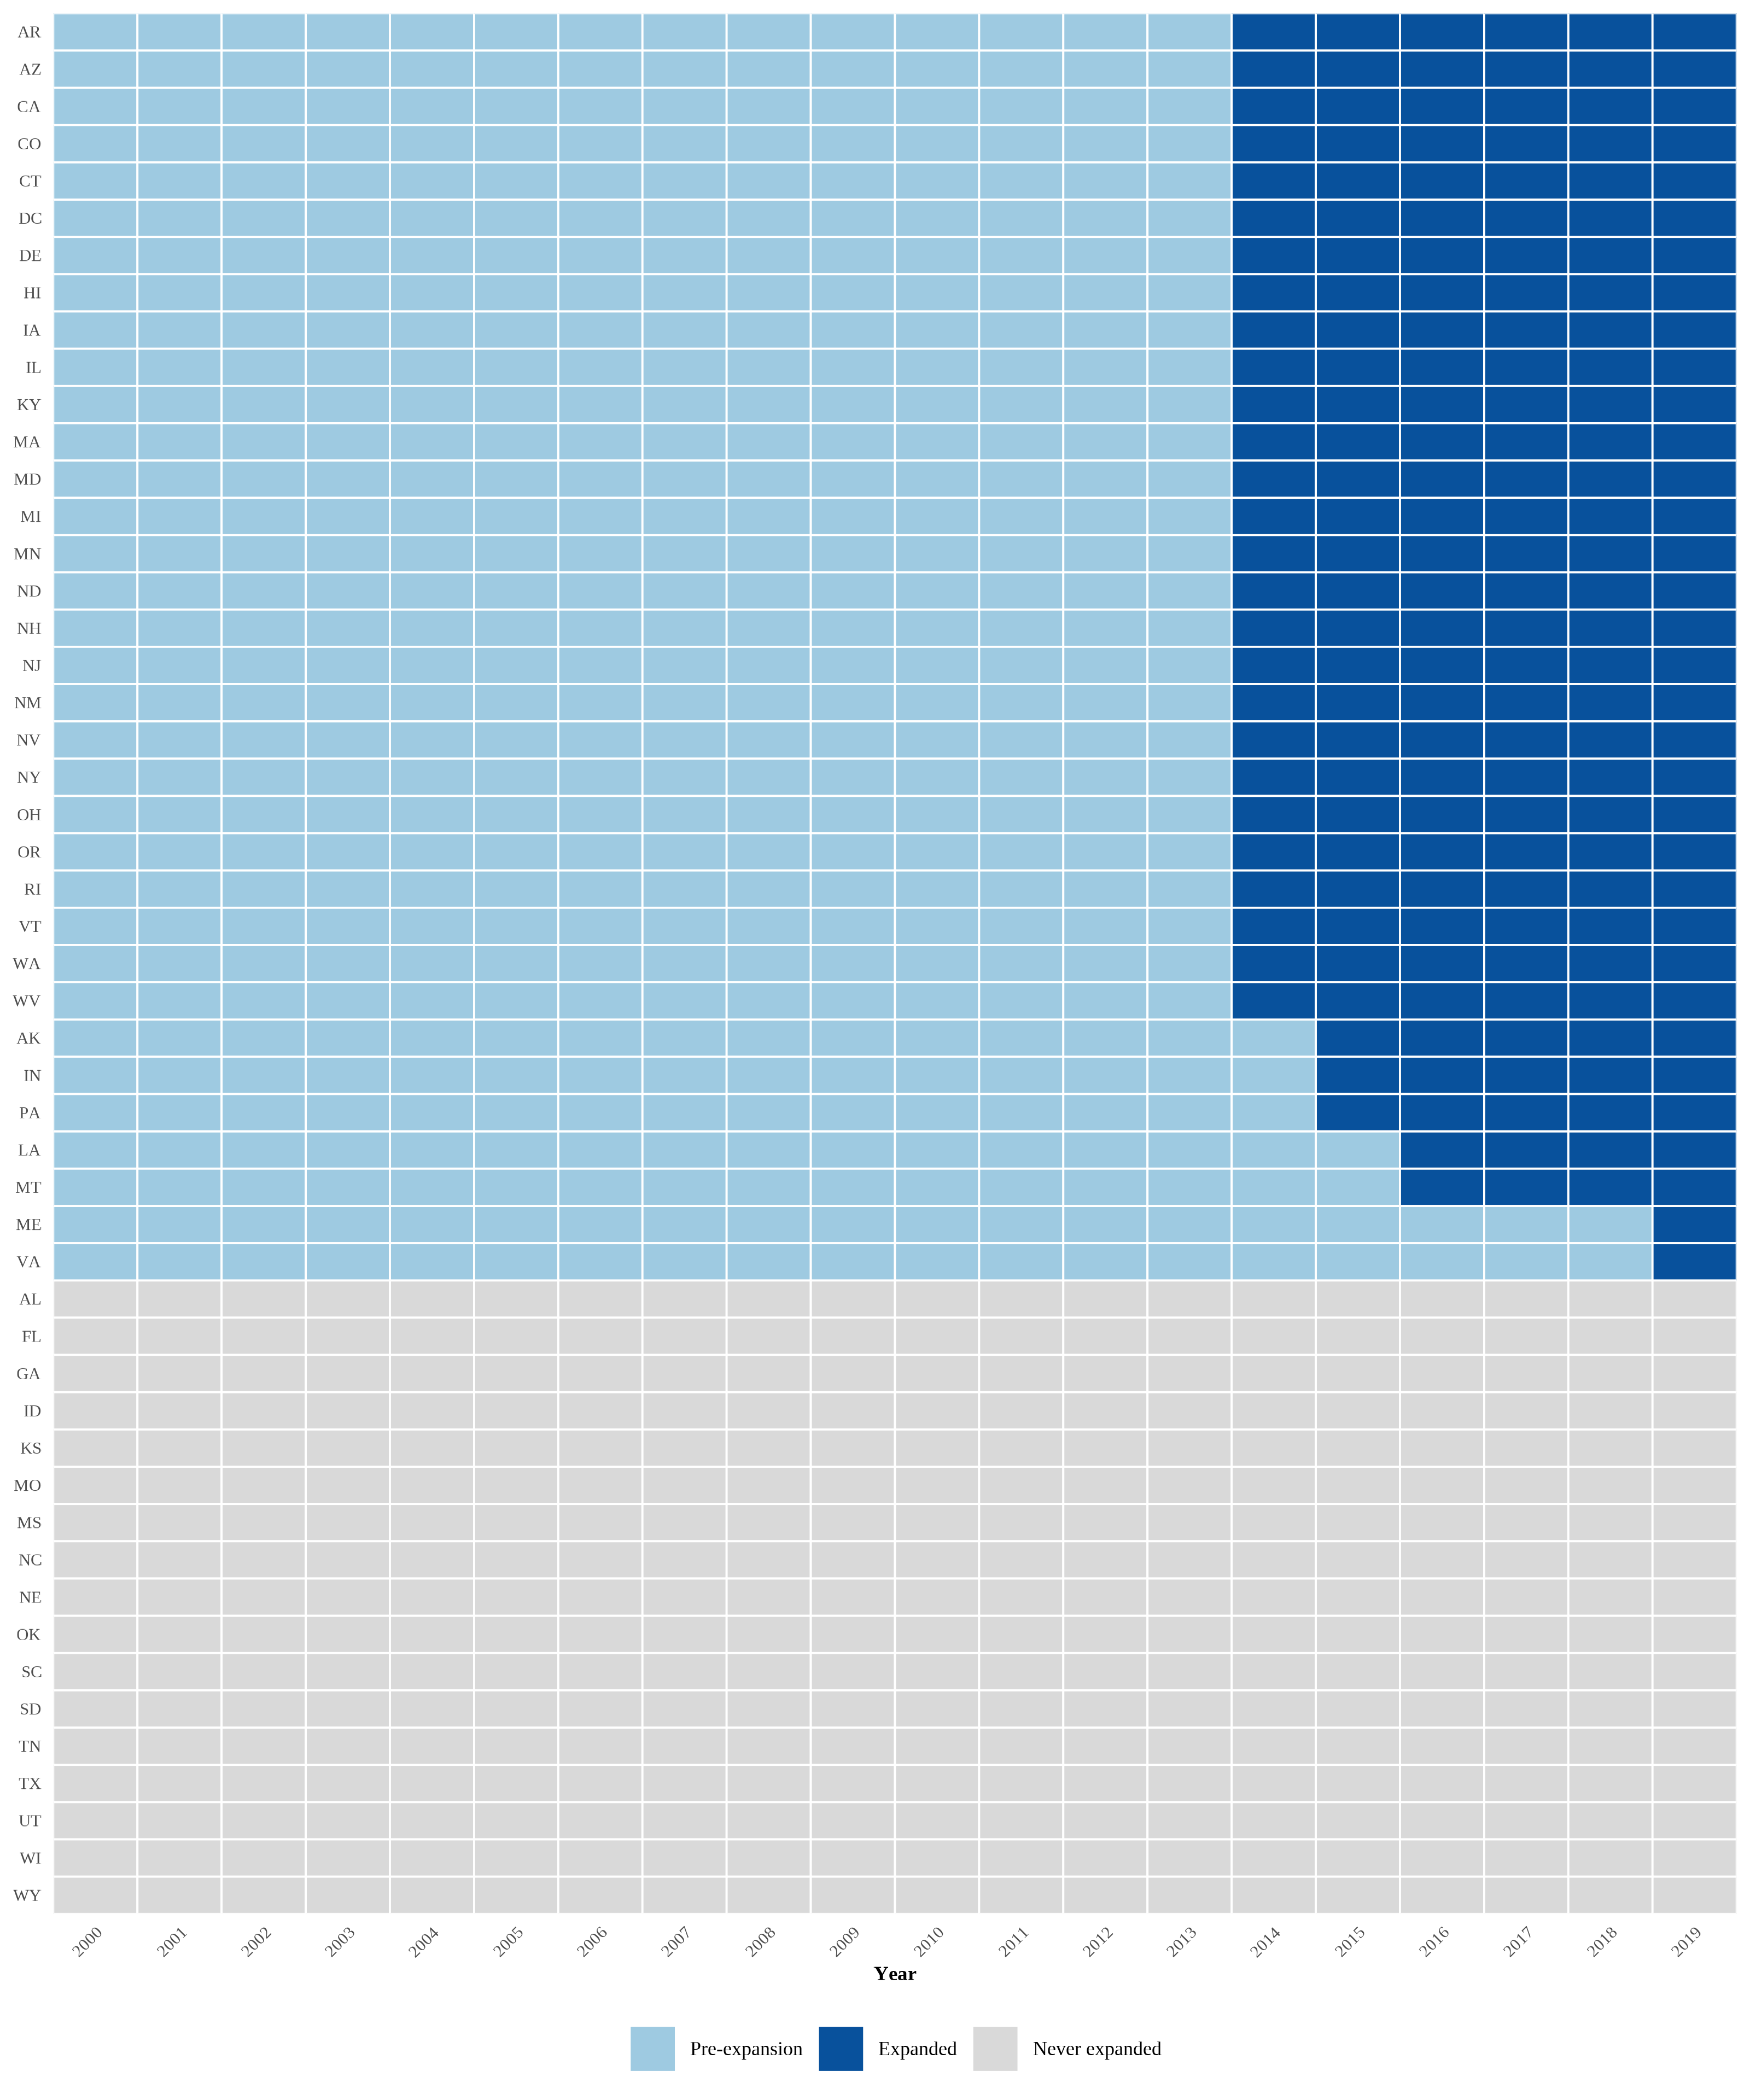
\includegraphics[width=\linewidth]{figures/desc-timing.png}
    \hfill
\caption*{\footnotesize{\textit{Notes:} The figure summarizes the treatment structure of the sample, where the unit of observation is a residency program (institution) and the treatment is the host state's adoption of Medicaid expansion. Programs are grouped by the timing of their state's expansion, and the vertical axis reports the number of programs in each group. Medium-blue cells denote treated programs in years before their state expanded Medicaid (``Treated (Pre)''), dark-navy cells denote treated programs in expansion and post-expansion years (``Treated (Post)''), and light-blue cells denote never-expansion (control) programs. The horizontal axis is the calendar year. The figure illustrates the staggered rollout of Medicaid expansion exploited by the difference-in-differences design. Data are from NRMP Main Residency Match reports, 2010--2019. The plot is produced with the \texttt{panelview} package (Mou, Liu, and Xu).}}
\end{figure}

\begin{figure}[H]
    \caption{Total Matched Residency Positions by Expansion Cohort}
    \label{fig2}
    \centering
      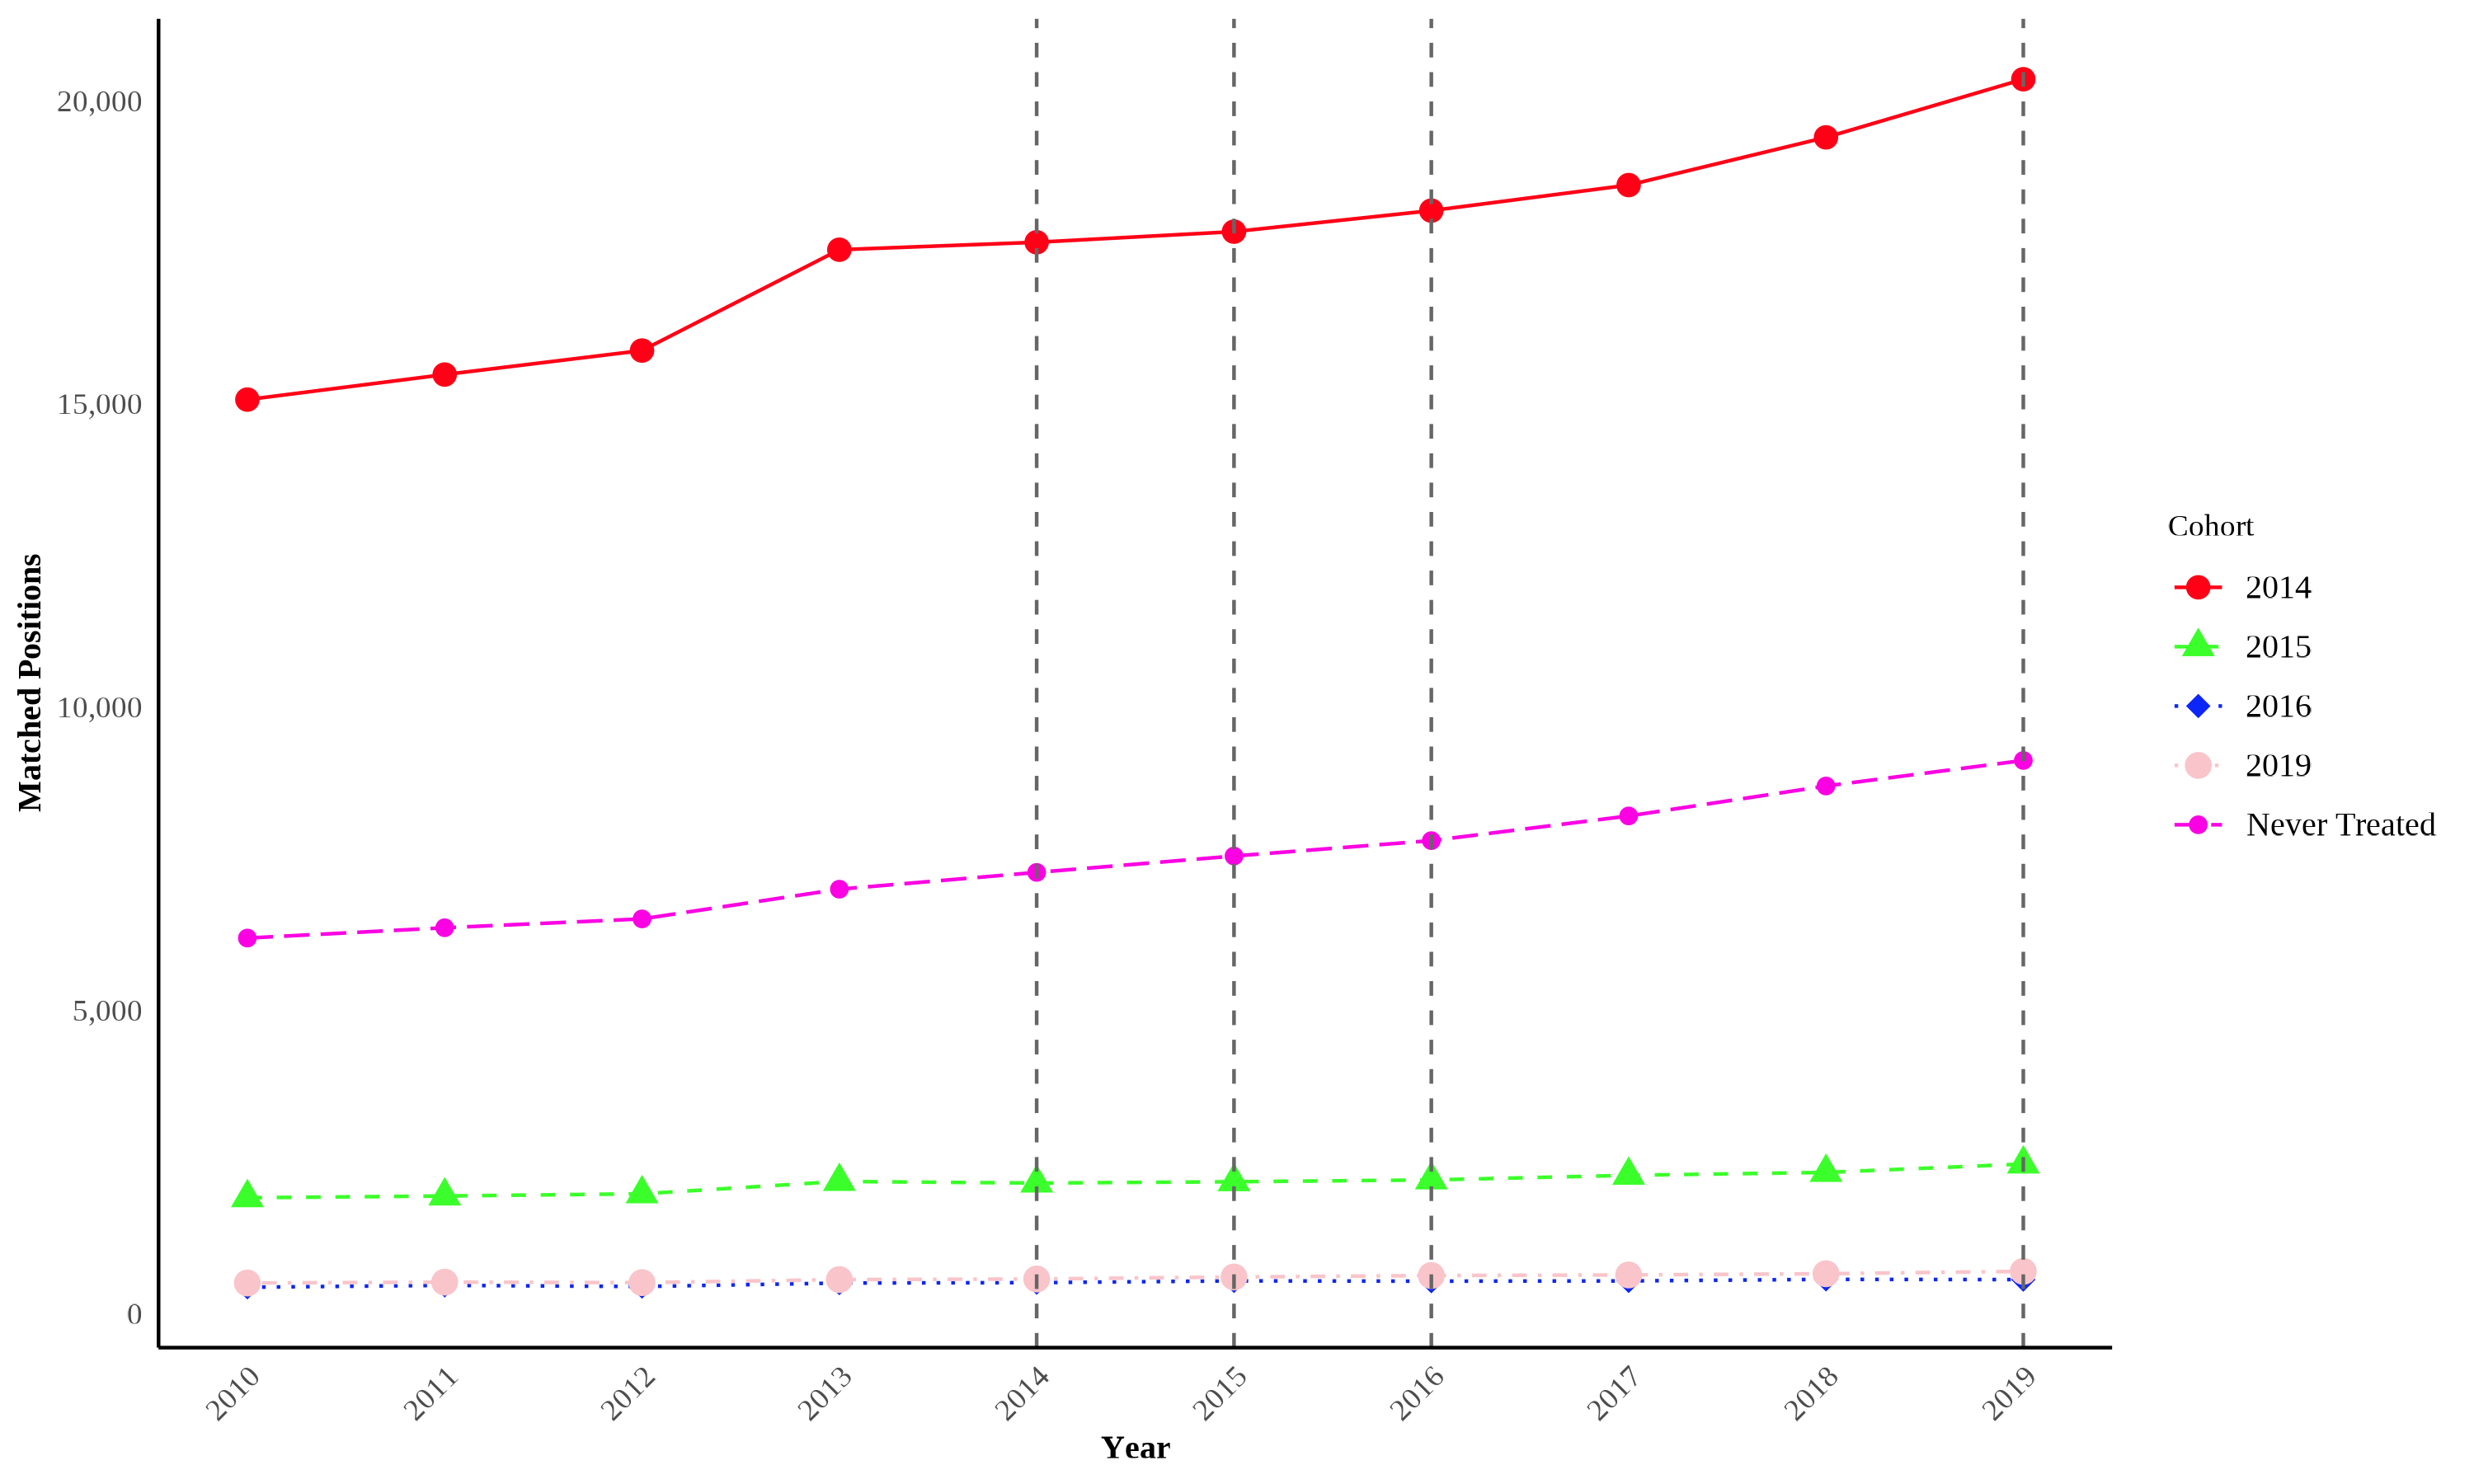
\includegraphics[width=\linewidth]{figures/desc-cohort-levels.png}
    \hfill
\caption*{\footnotesize{\textit{Notes:} The figure plots the total number of matched residency positions by year, separately for each Medicaid-expansion cohort. A cohort is defined by the calendar year in which a program's state expanded Medicaid (2014, 2015, 2016, and 2019); programs in states that never expanded over the sample period are grouped as ``Never Treated.'' Each series sums matched positions across all programs in the cohort, where positions are first aggregated to the institution-year level across specialties. Dashed vertical lines mark the expansion years of the treated cohorts. The figure is descriptive and is not adjusted for fixed effects or covariates. Data are from NRMP Main Residency Match reports, 2010--2019.}}
\end{figure}

\begin{figure}[H]
    \caption{Matched Residency Positions per 100,000 Population by Expansion Cohort}
    \label{fig3}
    \centering
      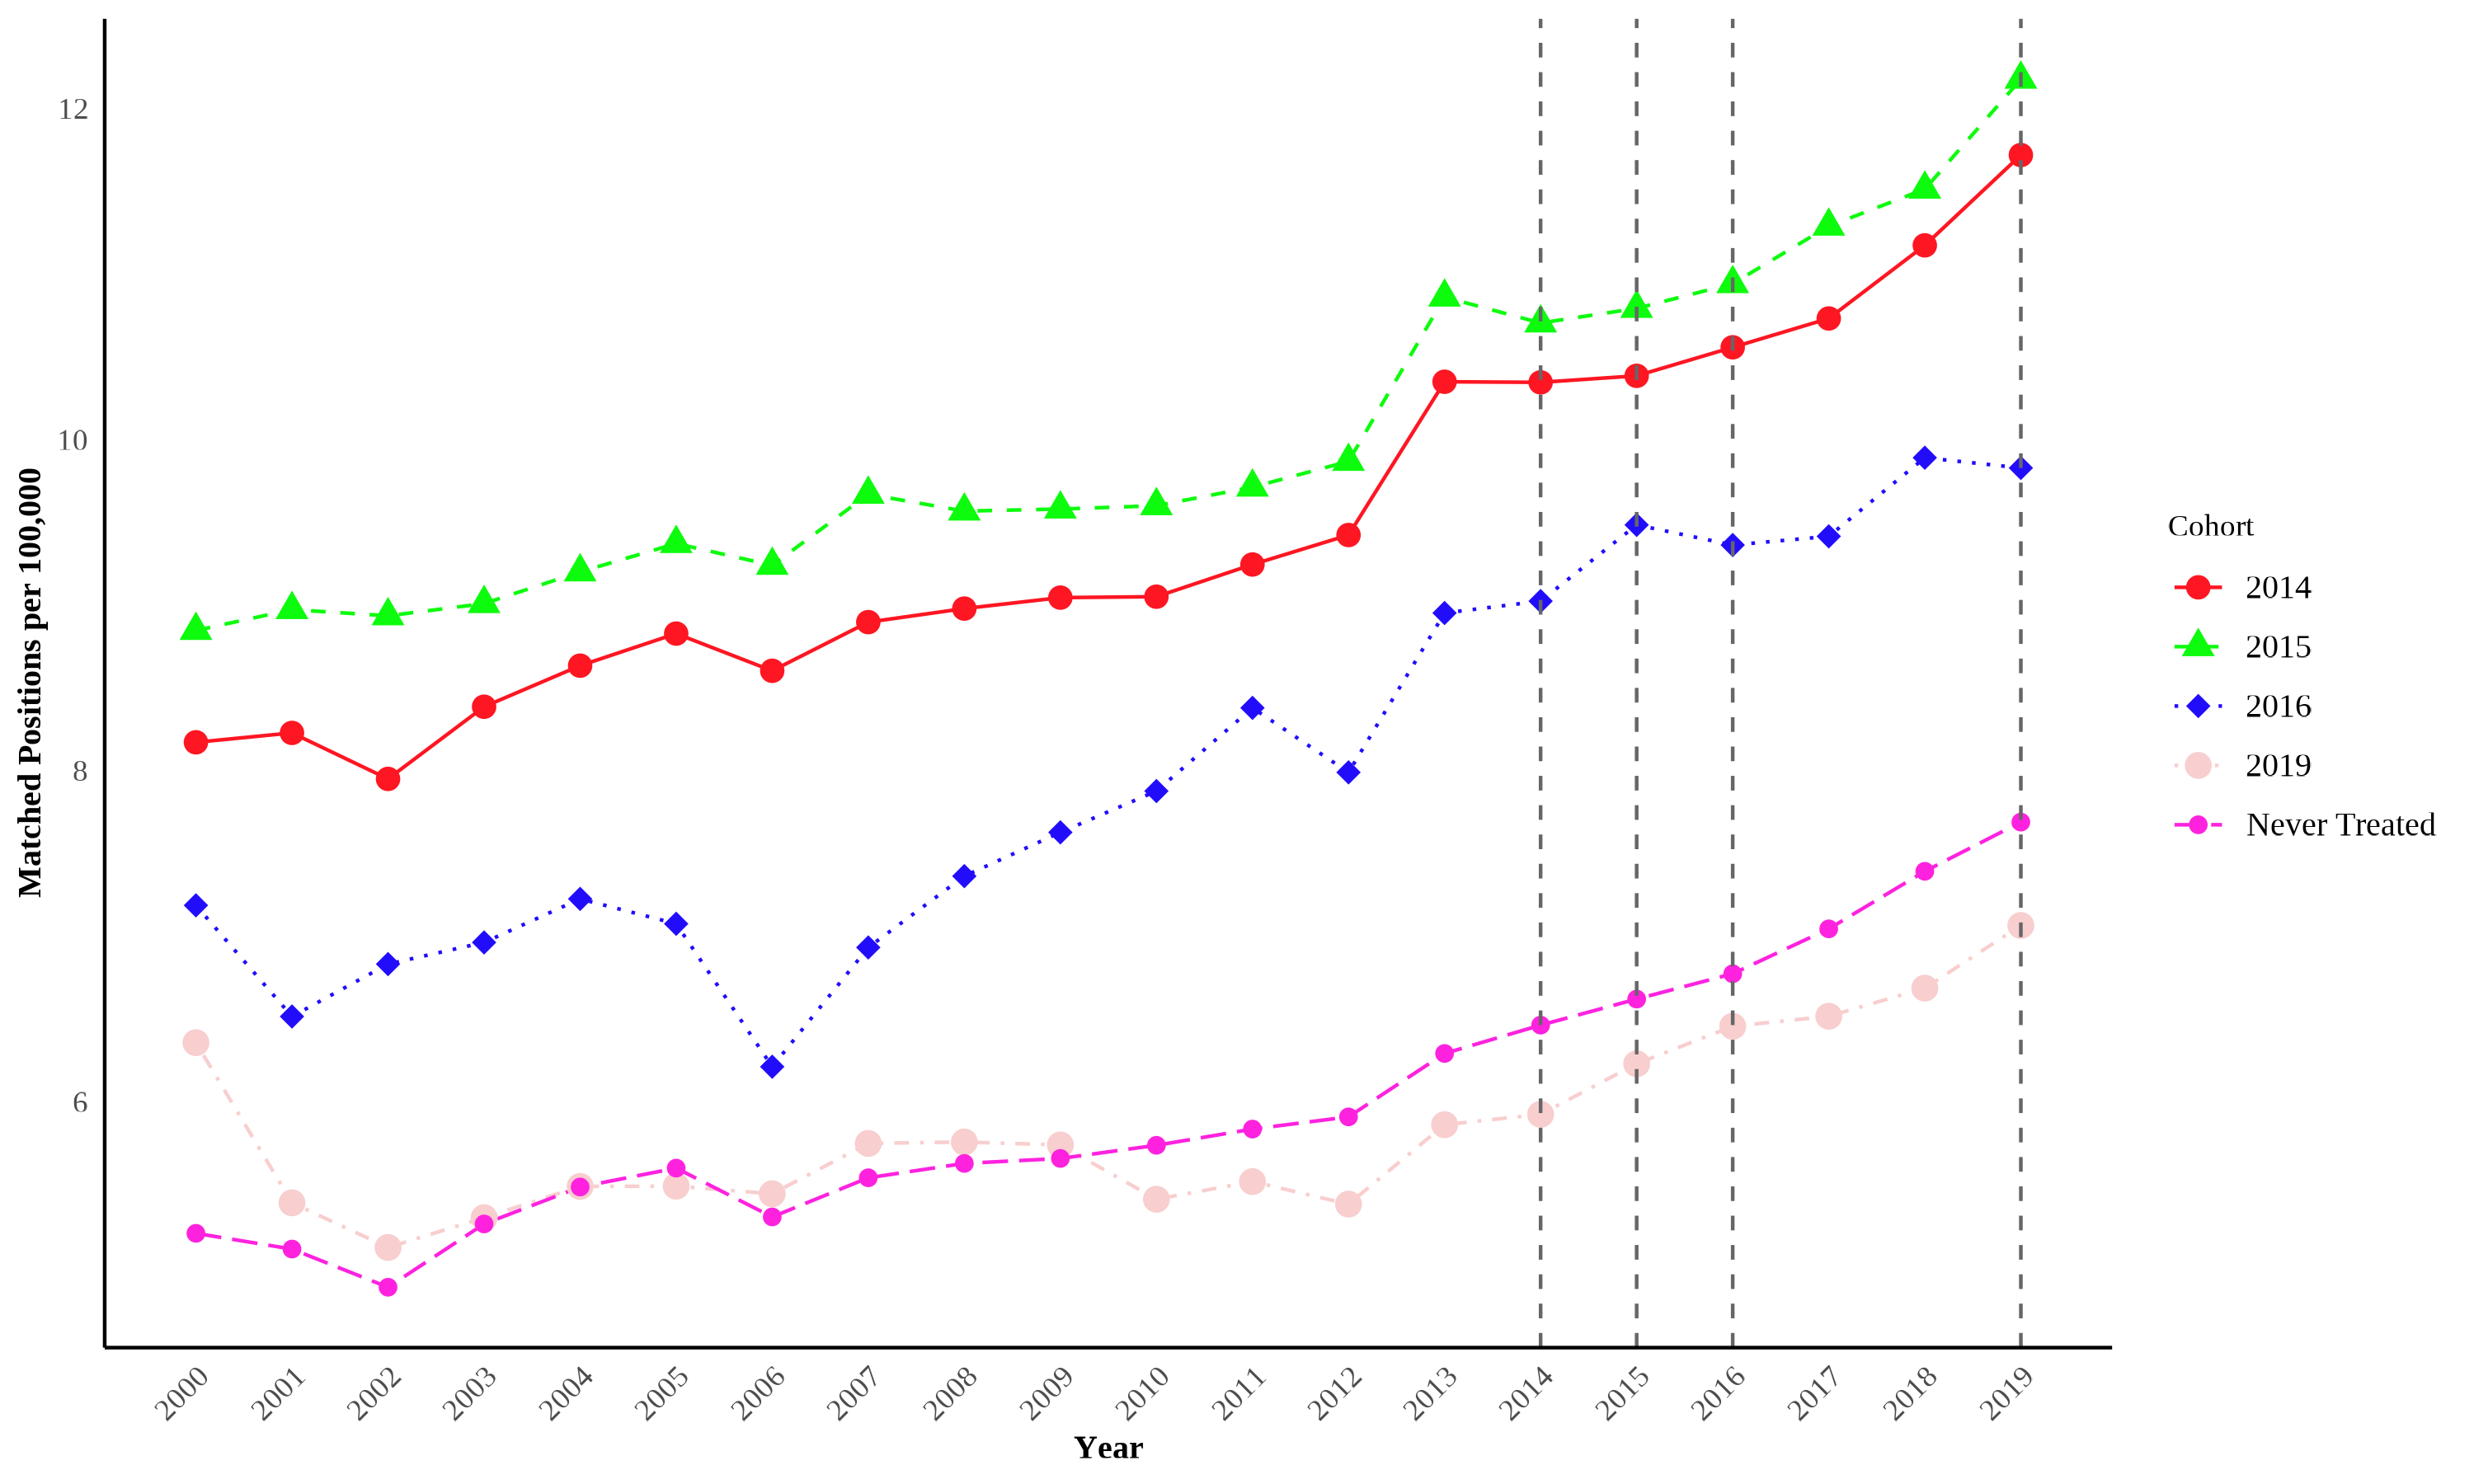
\includegraphics[width=\linewidth]{figures/desc-cohort-percapita.png}
    \hfill
\caption*{\footnotesize{\textit{Notes:} The figure plots matched residency positions per 100,000 population by year, separately for each Medicaid-expansion cohort. Cohorts are defined by the calendar year in which a program's state expanded Medicaid (2014, 2015, 2016, and 2019), with programs in non-expansion states grouped as ``Never Treated.'' For each cohort and year, matched positions and population are summed across the cohort's states before computing the rate per 100,000, using 2010 state population. Dashed vertical lines mark the expansion years of the treated cohorts. The figure is descriptive and is not adjusted for fixed effects or covariates. Data are from NRMP Main Residency Match reports, 2010--2019, and U.S.\ Census Bureau state population estimates.}}
\end{figure}

\begin{figure}[H]
    \caption{Growth in Physicians per 100,000 Population Relative to Total Population}
    \label{fig4}
    \centering
      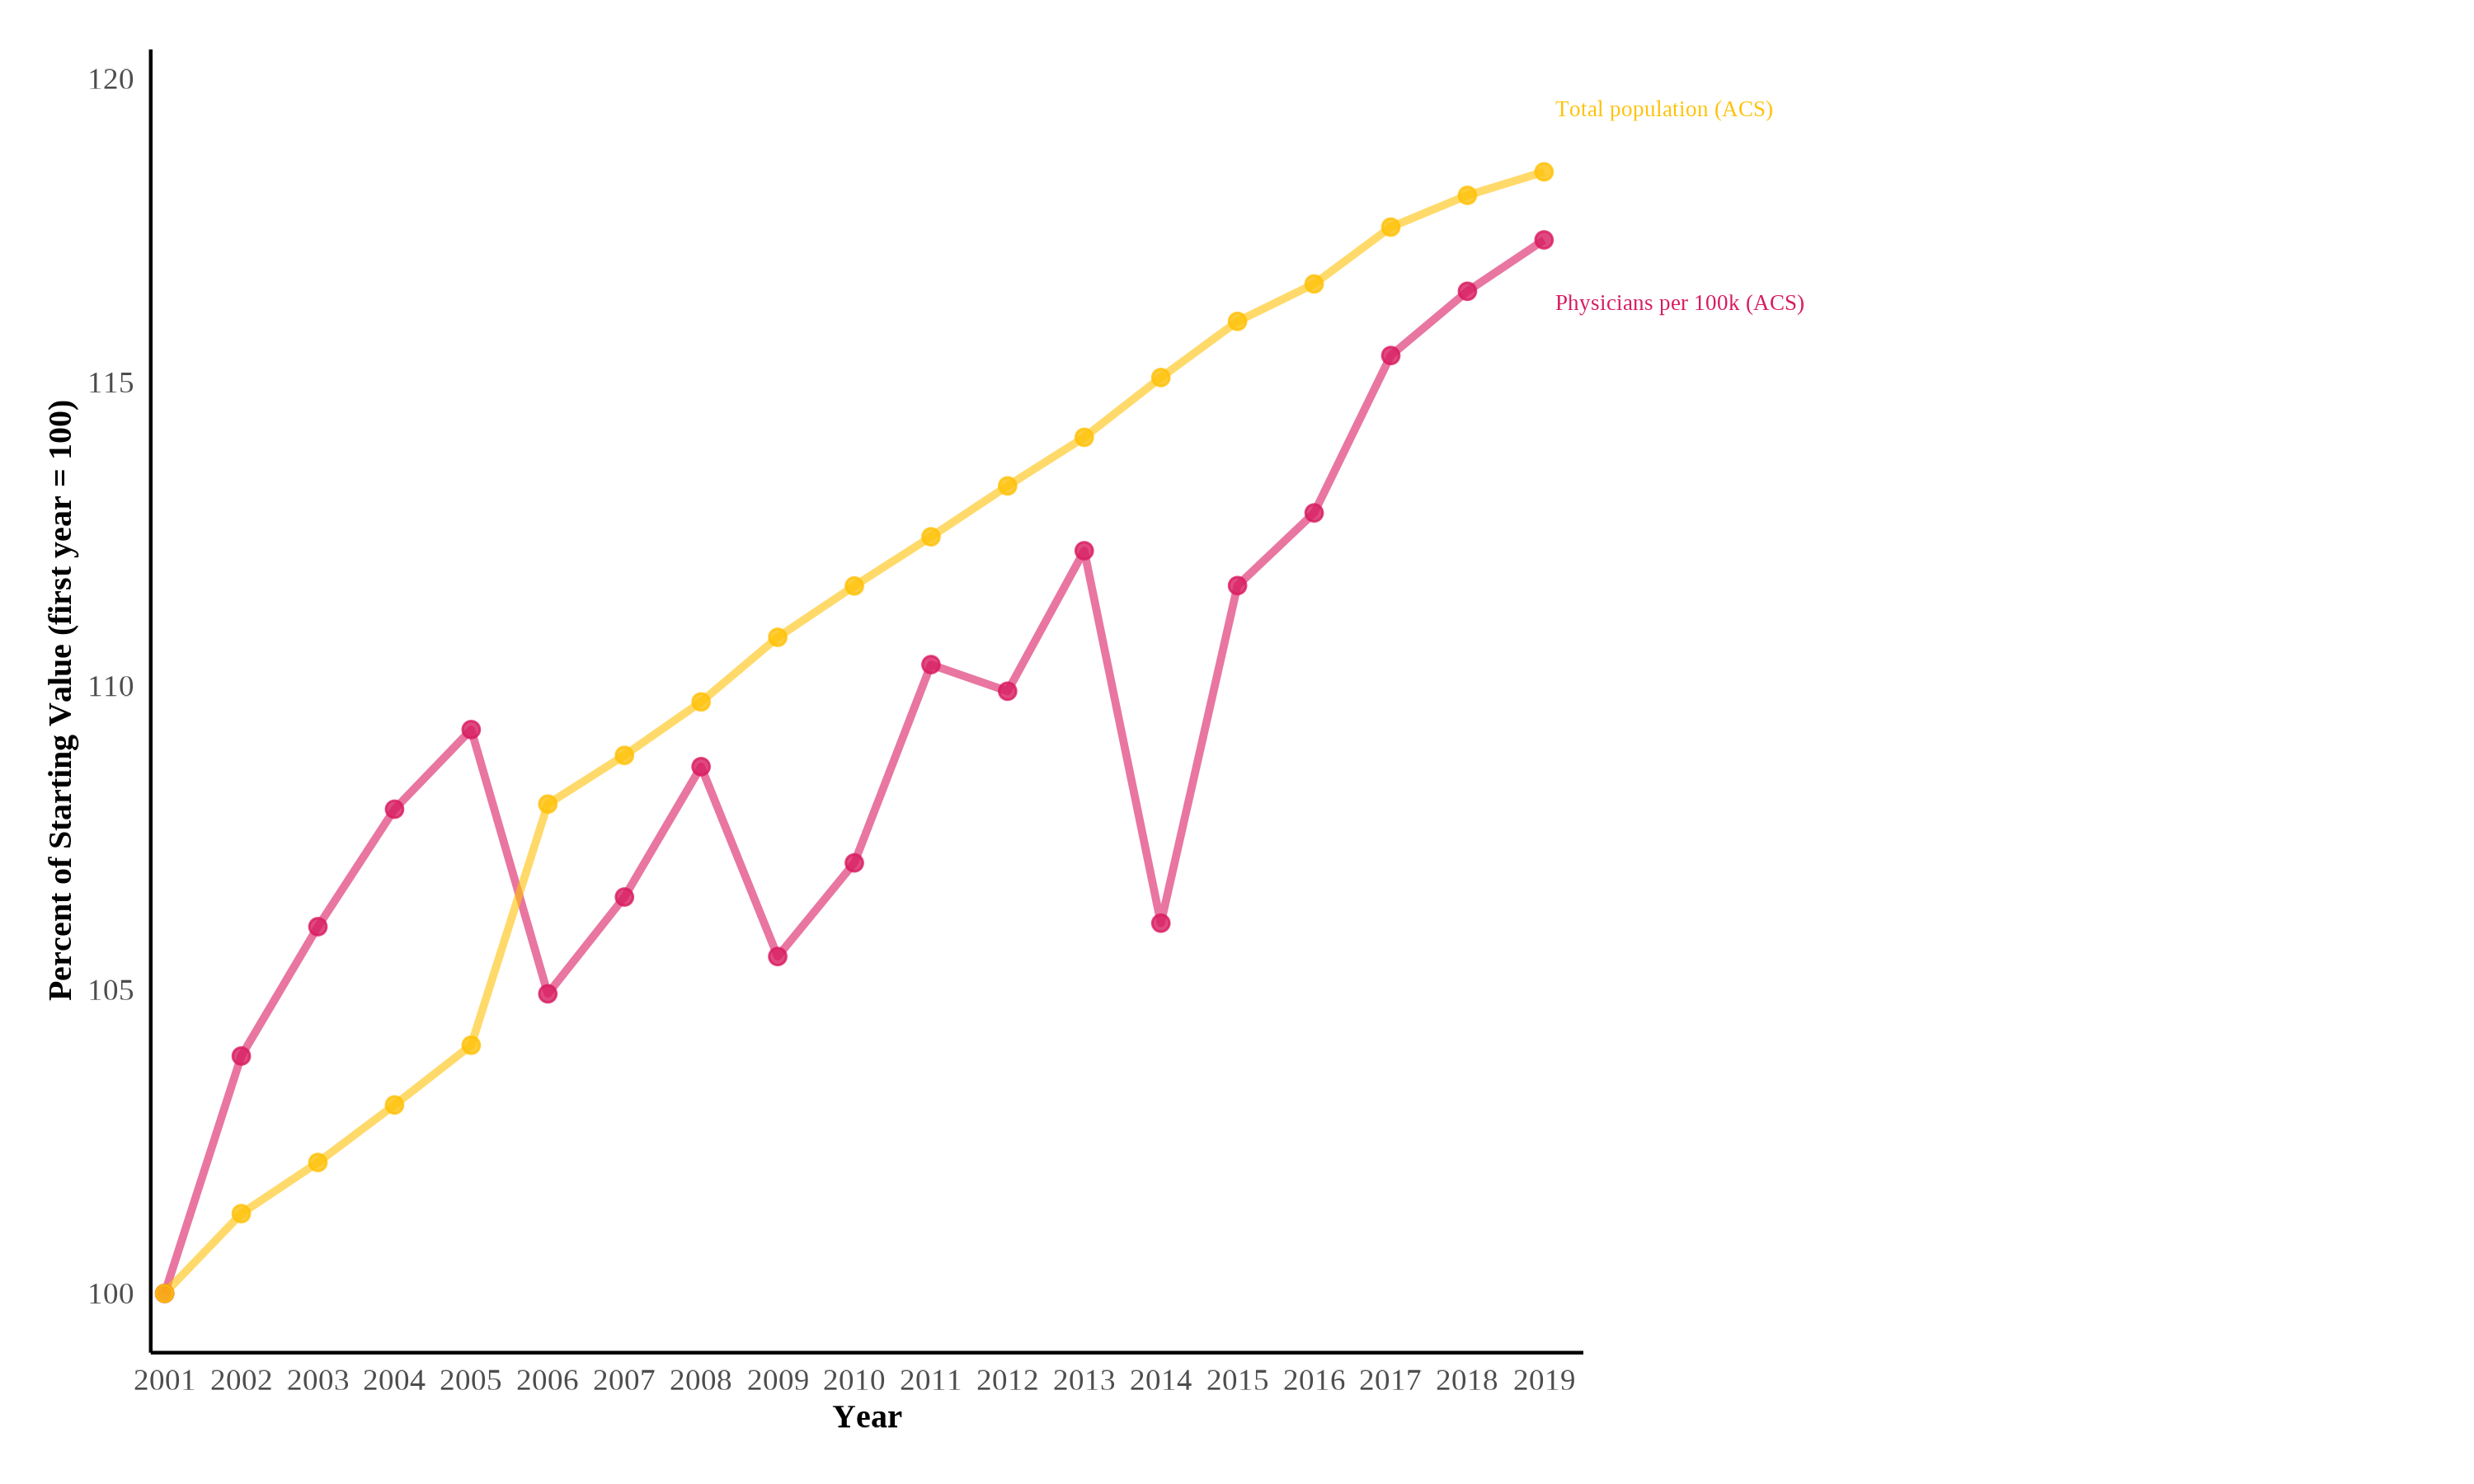
\includegraphics[width=\linewidth]{figures/desc-physician-growth.png}
    \hfill
\caption*{\footnotesize{\textit{Notes:} The figure plots the cumulative percent change since 2001 (2001 $= 100$) in two national series from the American Community Survey (ACS): physicians per 100,000 population and total population. Physicians are defined as employed workers in the harmonized occupation code for physicians and surgeons (\texttt{OCC1950} $= 75$). Estimates use the ACS person weight (\texttt{PERWT}). Data are from IPUMS-USA. The figure motivates the analysis by showing that the physician-to-population ratio has roughly tracked, rather than outpaced, population growth.}}
\end{figure}


\begin{figure}[H]
    \caption{Effect of Medicaid Expansion on Matched Residency Positions: Event Study Estimates}
    \label{fig5}
    \centering
      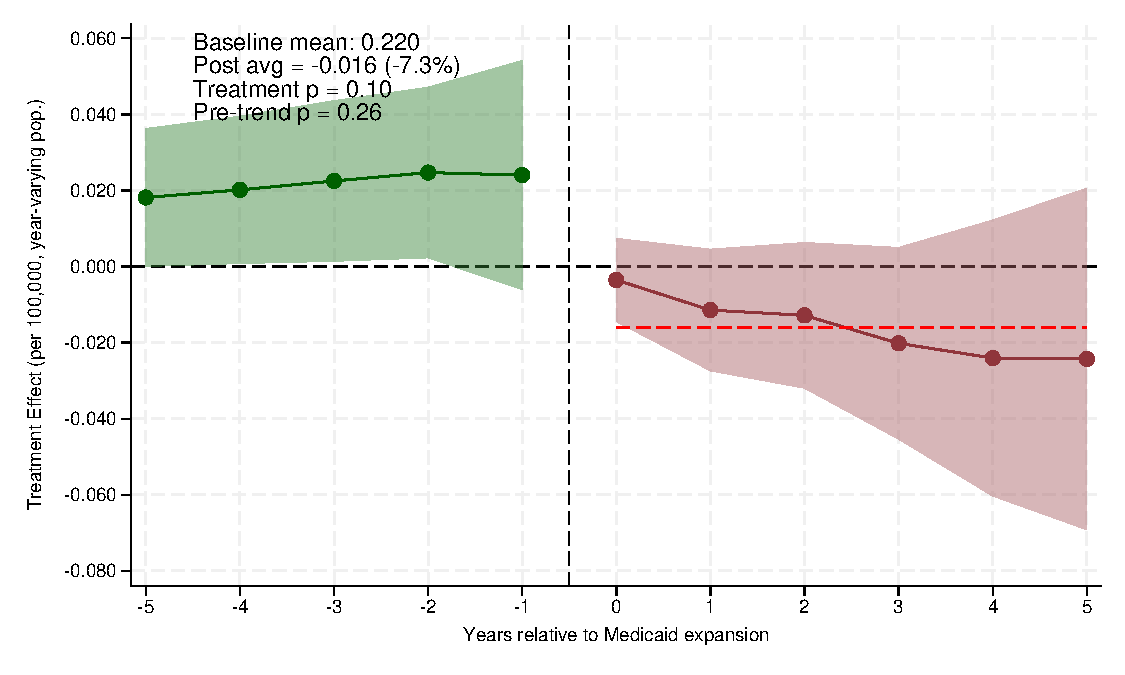
\includegraphics[width=\linewidth]{figures/main-headline.pdf}
    \hfill
\caption*{\footnotesize{\textit{Notes:} The figure plots event-study coefficients from the imputation estimator of Borusyak, Jaravel, and Spiess (2024), where the outcome is matched residency positions per 100,000 \emph{contemporary} (year-varying) state population from the American Community Survey. The horizontal axis measures years relative to a state's Medicaid expansion; year 0 is the first year of expansion. Green circles (years $-5$ to $-1$) show pre-expansion coefficients. Dark red circles (years $0$ to $+5$) show post-expansion treatment effects. The dashed red line indicates the average post-expansion treatment effect ($-0.016$), approximately $-7.3$ percent relative to the pre-expansion mean of $0.22$ matched positions per 100,000 (joint $p = 0.10$); the pre-expansion coefficients are jointly small and consistent with parallel trends (pre-trend $p = 0.26$). As discussed in the text, the aggregate magnitude is imprecise under randomization inference; the sign, dynamics, and mechanism are the robust features. Shaded bands are 95 percent confidence intervals. Regressions include hospital and year fixed effects and weight by 2010 state population. Standard errors are clustered at the state level.}}
\end{figure}

\newpage
\pagebreak

\begin{figure}[H]
    \caption{Effect of Medicaid Expansion on Direct GME (DGME) Payments: Event Study Estimates}
    \label{afig13}
    \centering
      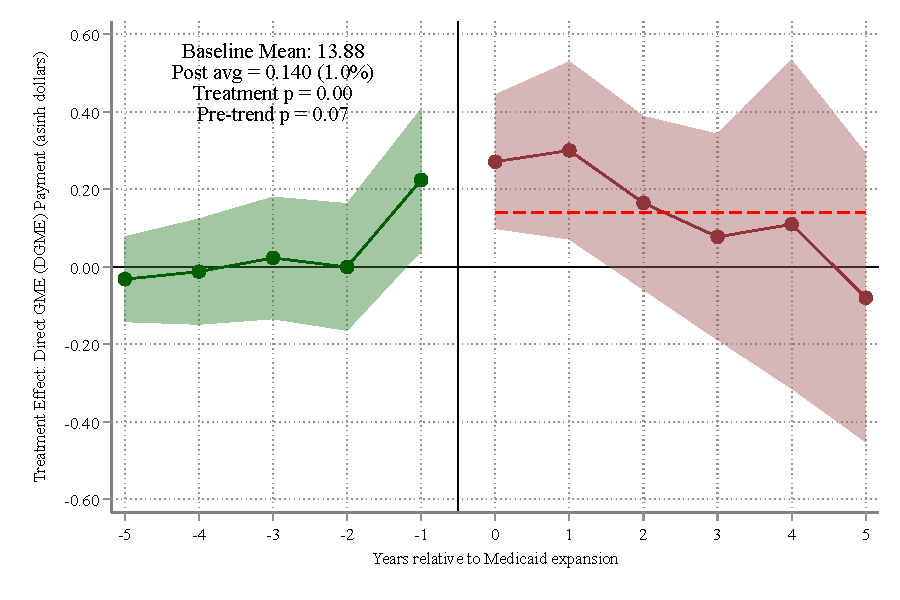
\includegraphics[width=\linewidth]{figures/main-firststage-dgme.pdf}
    \hfill
\caption*{\footnotesize{\textit{Notes:} The figure plots event-study coefficients from the imputation estimator of Borusyak, Jaravel, and Spiess (2024). The outcome is the inverse hyperbolic sine (asinh) of Direct GME (DGME) payments per teaching hospital, from CMS Medicare hospital cost reports; DGME reimburses the direct costs of residency training (resident salaries, benefits, and faculty supervision). Because $\operatorname{asinh}(x)\approx\ln(2x)$ for large $x$, coefficients approximate proportional changes. The sample comprises all hospitals receiving Medicare GME payments, observed at the hospital--fiscal-year level, with never-expansion states as the comparison group. The horizontal axis measures years relative to a state's Medicaid expansion; year 0 is the first year of expansion. Green circles (years $-5$ to $-1$) show pre-expansion coefficients; dark red circles (years $0$ to $+5$) show post-expansion treatment effects. The dashed red line indicates the average post-expansion effect of $0.140$, roughly a $14$ percent increase in DGME payments (joint $p < 0.01$), with the largest effects in the first two post-expansion years. Pre-expansion coefficients are near zero from event years $-5$ to $-2$; the elevated coefficient at $-1$ (joint pre-trend $p = 0.07$) is consistent with modest anticipatory increases in payments. Shaded bands are 95 percent confidence intervals. Estimates are based on 1,916 hospitals across 51 states and the District of Columbia. Regressions include hospital and year fixed effects and are unweighted. Standard errors are clustered at the state level.}}
\end{figure}

\newpage
\pagebreak

\begin{figure}[H]
    \caption{Effect of Medicaid Expansion on Indirect Medical Education (IME) Payments: Event Study Estimates}
    \label{afig14}
    \centering
      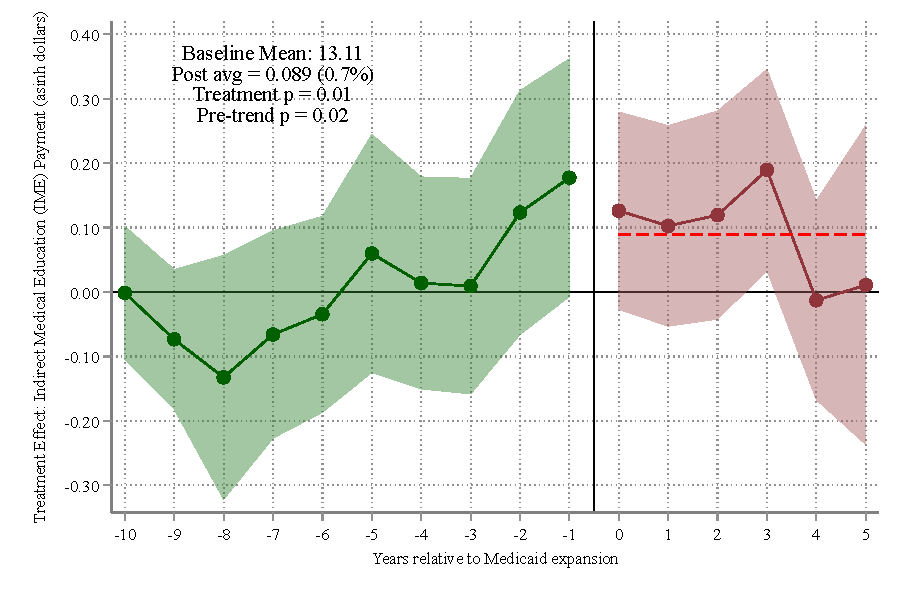
\includegraphics[width=\linewidth]{figures/main-firststage-ime.pdf}
    \hfill
\caption*{\footnotesize{\textit{Notes:} The figure plots event-study coefficients from the imputation estimator of Borusyak, Jaravel, and Spiess (2024) for the indirect component of GME payments, complementing the Direct GME estimate in \cref{afig13}. The outcome is the inverse hyperbolic sine (asinh) of Indirect Medical Education (IME) payments per teaching hospital, from CMS Medicare hospital cost reports; IME is the indirect operating-cost adjustment paid to teaching hospitals, as distinct from the direct training costs captured by DGME. Because $\operatorname{asinh}(x)\approx\ln(2x)$ for large $x$, coefficients approximate proportional changes. The average post-expansion effect is $0.059$, roughly a $6$ percent increase, and is only marginally significant (joint $p = 0.06$); pre-expansion coefficients are jointly insignificant (joint pre-trend $p = 0.32$). The muted response relative to Direct GME indicates that the GME-financing effect of expansion operates primarily through direct resident-training payments rather than the indirect adjustment. The sample comprises all hospitals receiving Medicare GME payments at the hospital--fiscal-year level, with never-expansion states as the comparison group. Green circles (years $-5$ to $-1$) show pre-expansion coefficients; dark red circles (years $0$ to $+5$) show post-expansion treatment effects. Shaded bands are 95 percent confidence intervals. Estimates are based on 1,916 hospitals across 51 states and the District of Columbia. Regressions include hospital and year fixed effects and are unweighted. Standard errors are clustered at the state level.}}
\end{figure}

\newpage
\pagebreak

\begin{figure}[H]
    \caption{Mechanism: Effect of Medicaid Expansion by State Medicaid GME Formula}
    \label{fig:mech_gme}
    \centering
    \begin{subfigure}{\linewidth}
        \centering
        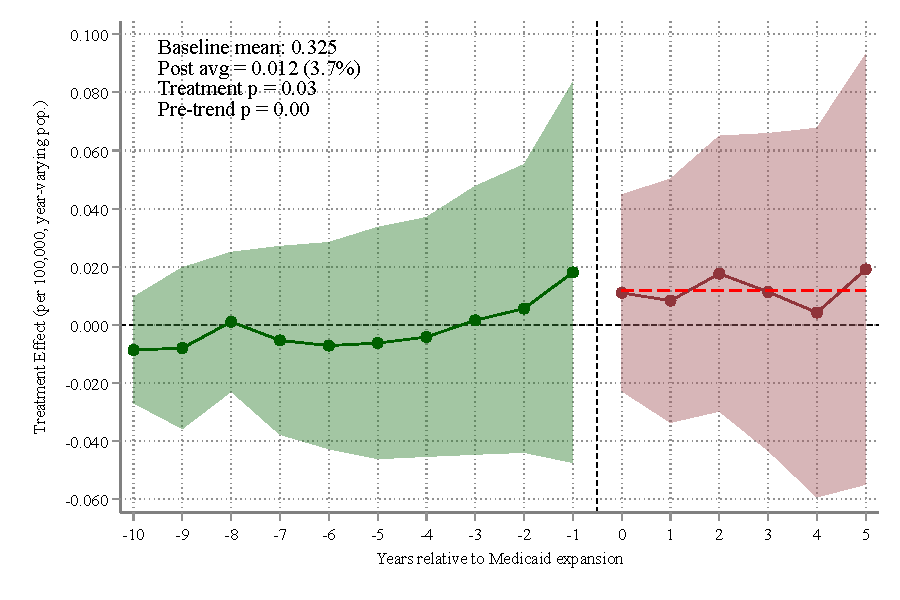
\includegraphics[width=0.75\linewidth]{figures/main-mechanism-volume.pdf}
        \caption{Volume-Responsive GME States}
        \label{fig:mech_gme:vol}
    \end{subfigure}
    \hfill
    \begin{subfigure}{\linewidth}
        \centering
        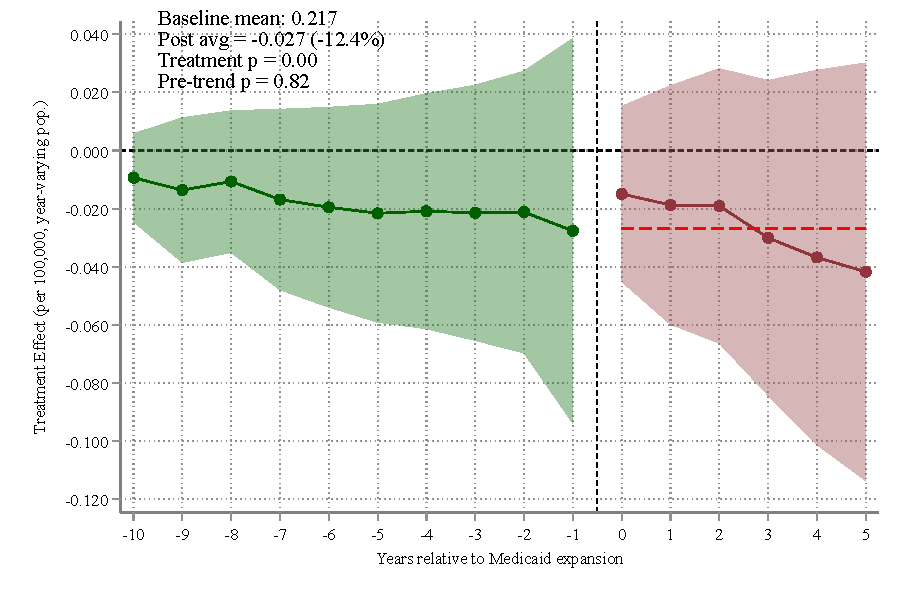
\includegraphics[width=0.75\linewidth]{figures/main-mechanism-nonresp.pdf}
        \caption{Non-Responsive GME States (Fixed/None)}
        \label{fig:mech_gme:nonresp}
    \end{subfigure}
\caption*{\footnotesize{\textit{Notes:} The figure plots event-study coefficients
from the imputation estimator of \textcite{borusyak2024revisiting}, estimated
separately for expansion states with volume-responsive (top) versus non-responsive
(bottom) Medicaid GME formulas, each using non-expansion states as the comparison
group. The outcome is matched residency positions per 100{,}000 contemporary
(year-varying) state population. In non-responsive states the average post-expansion
effect is $-0.022$ (an $11.7$ percent decline; joint $p < 0.01$) following flat
pre-expansion coefficients (pre-trend $p = 0.15$); in volume-responsive states it is
$+0.013$ ($+3.4$ percent), with no decline. A pooled interacted model puts the
volume-minus-non-responsive difference in average post effects at $0.035$ per
100{,}000 (clustered p $< 0.001$; randomization-inference p $= 0.19$). The
volume-responsive panel exhibits a pronounced upward pre-trend (pre-trend
$p < 0.001$), so its estimate should be read with caution; the non-responsive
contraction is the more robust leg of the comparison.
Volume-responsive states reward higher Medicaid volume with larger GME payments, so
expansion mechanically raises GME revenue; non-responsive states (fixed per-resident
amounts, lump-sum grants, or no Medicaid GME) gain none. States are classified from
the Medicaid GME payment methodology reported in \textcite{henderson2013}. Green
circles (years $-5$ to $-1$) show pre-expansion coefficients; dark red circles
(years $0$ to $+5$) show post-expansion treatment effects; the dashed red line marks
the average post-expansion effect. Shaded bands are 95 percent confidence intervals.
Regressions include hospital and year fixed effects, are weighted by state
population. Standard errors are clustered at the state level.}}
\end{figure}

\begin{figure}[H]
    \caption{Effect of Medicaid Expansion on Matched Residency Positions by Hospital Location: Event Study Estimates}
    \label{fig6}
    \centering
      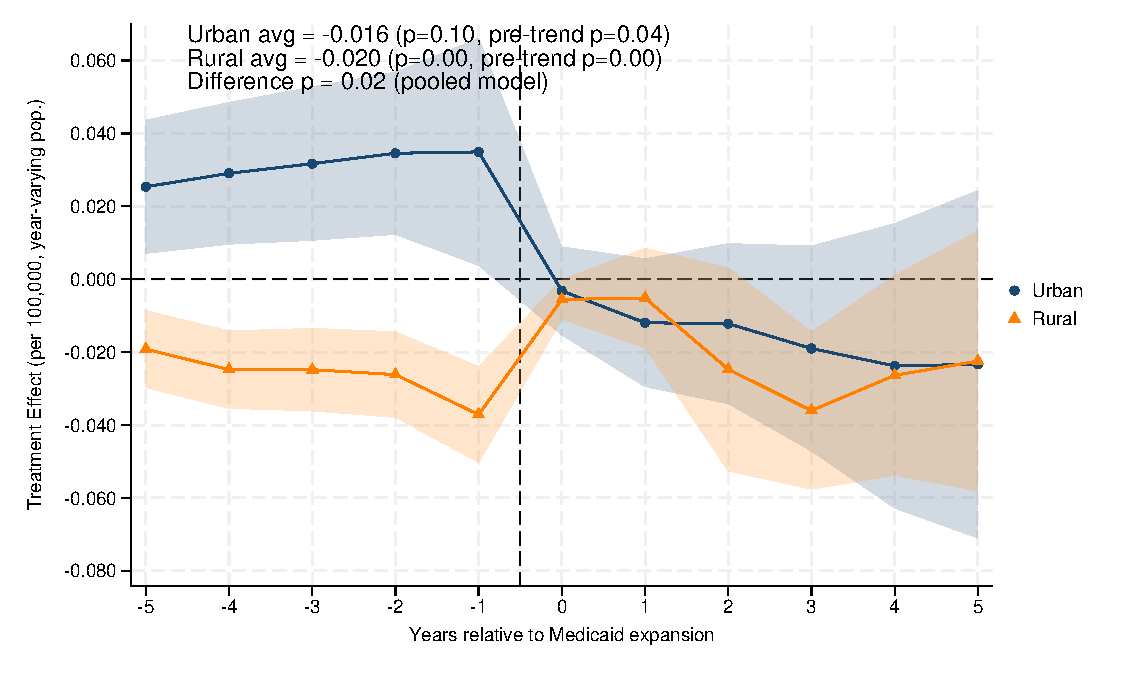
\includegraphics[width=\linewidth]{figures/main-location.pdf}
    \hfill
\caption*{\footnotesize{\textit{Notes:} The figure plots event-study coefficients from the imputation estimator of Borusyak, Jaravel, and Spiess (2024), estimated in two split-sample regressions for urban (blue circles) and rural (orange triangles) hospitals; each subsample keeps the never-expansion hospitals of its own type as the comparison group, so each series carries its own pre-expansion path and pre-trends test. Urban hospitals are those in counties with 2010 RUCA codes 1--3; rural hospitals are those with RUCA codes above 3. The outcome is matched positions per 100,000 contemporary (year-varying) population. The horizontal axis measures years relative to a state's Medicaid expansion; year 0 is the first year of expansion. The average post-expansion treatment effect is $-0.016$ for urban hospitals (joint p $= 0.10$; pre-trend p $= 0.04$, with uniformly positive pre-expansion coefficients) and $-0.020$ for rural hospitals (joint p $< 0.001$). The rural subsample fails its own pre-trends test (p $< 0.001$), with negative pre-expansion coefficients comparable in size to the post-expansion effects, so the rural series should be read descriptively. A pooled interacted model puts the urban--rural difference in average post effects at $-0.014$ (p $= 0.02$), but that model shares pre-trends across groups. Shaded bands are 95 percent confidence intervals. Regressions include hospital and year fixed effects and weight by 2010 state population. Standard errors are clustered at the state level.}}
\end{figure}

\begin{figure}[H]
    \caption{Effect of Medicaid Expansion on Matched Residency Positions by Specialty Type: Event Study Estimates}
    \label{fig7}
    \centering
    \begin{subfigure}{\linewidth}
        \centering
        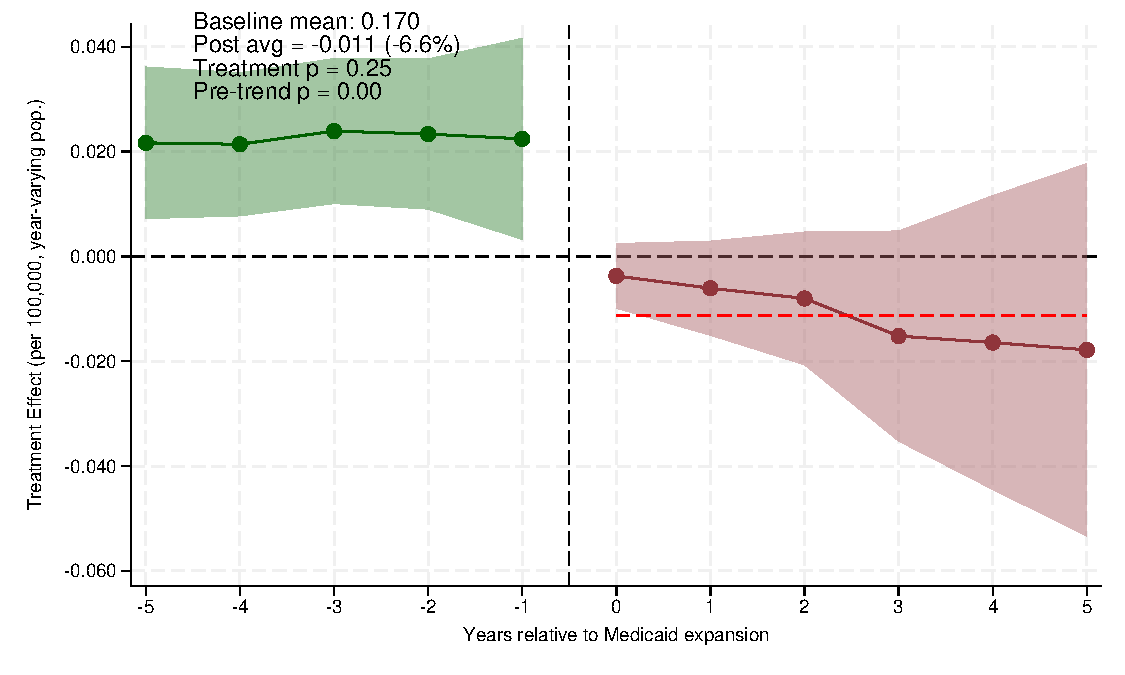
\includegraphics[width=0.75\linewidth]{figures/main-specialty-nonprimary.pdf}
        \caption{Non-Primary Care Positions}
        \label{fig7:non-prim-care}
    \end{subfigure}
    \hfill
    \begin{subfigure}{\linewidth}
        \centering
        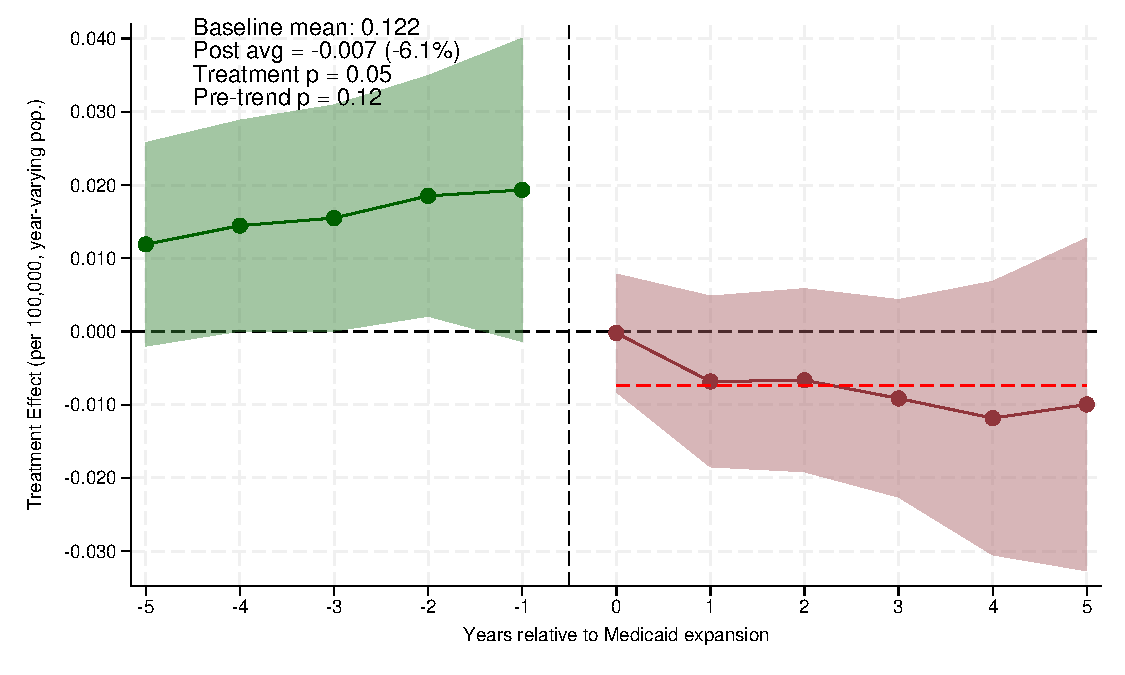
\includegraphics[width=0.75\linewidth]{figures/main-specialty-primary.pdf}
        \caption{Primary Care Positions}
        \label{fig7:prim-care}
    \end{subfigure}
\caption*{\footnotesize{\textit{Notes:} The figure plots event-study coefficients from the imputation estimator of Borusyak, Jaravel, and Spiess (2024) estimated separately for non-primary care (top panel) and primary care specialties (bottom panel). Primary care includes family medicine, internal medicine, and pediatrics. The outcome is matched positions per 100,000 contemporary (year-varying) population. The horizontal axis measures years relative to a state's Medicaid expansion; year 0 is the first year of expansion. For non-primary care programs, the average post-expansion treatment effect is $-0.002$ ($-4.7$ percent; p $= 0.22$; pre-trend $p = 0.01$). For primary care programs, it is $-0.003$ ($-4.6$ percent; p $= 0.06$; pre-trend $p = 0.06$). Both panels exhibit differential pre-trends, so the specialty estimates should be read as suggestive. Shaded bands are 95 percent confidence intervals. Regressions include hospital and year fixed effects and weight by 2010 state population. Standard errors are clustered at the state level.}}
\end{figure}

\begin{figure}[H]
    \caption{Robustness of Event Study Estimates Across Difference-in-Differences Estimators: Matched Residency Positions per 100,000 Population}
    \label{fig8}
    \centering
      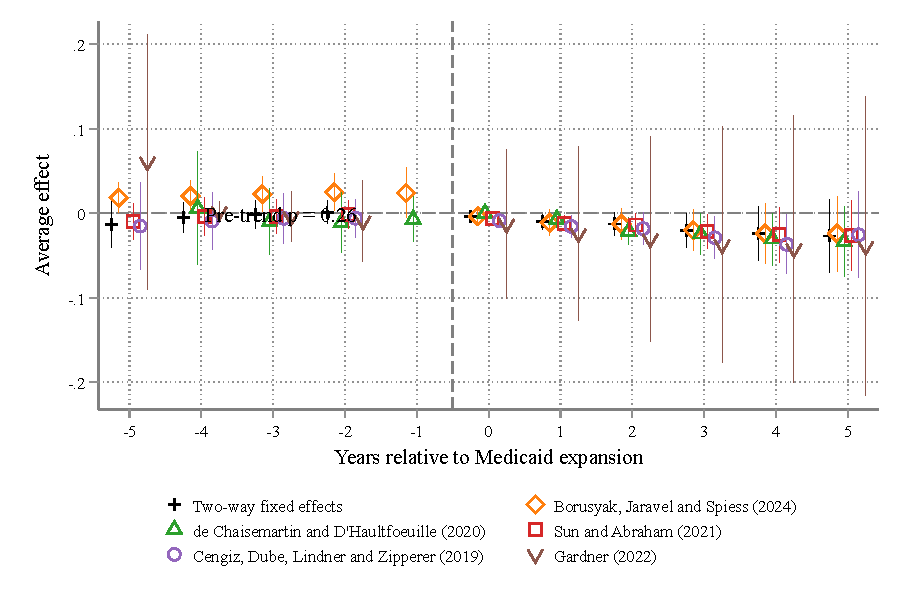
\includegraphics[width=\linewidth]{figures/main-estimators.pdf}
    \hfill
\caption*{\footnotesize{\textit{Notes:} The figure compares event-study estimates of the effect of Medicaid expansion on matched residency positions per 100,000 contemporary (year-varying) population across six difference-in-differences estimators that are robust to treatment-effect heterogeneity under staggered adoption: two-way fixed effects; Borusyak, Jaravel, and Spiess (2024); de Chaisemartin and D'Haultfoeuille (2020); Sun and Abraham (2021); Cengiz, Dube, Lindner, and Zipperer (2019); and Gardner (2022). The heterogeneity-robust estimator of Callaway and Sant'Anna (2021) is excluded because it is not well identified in the sparsely populated never-treated cells of this sample. The pre-trend $p$-value reported in the panel is from the Borusyak, Jaravel, and Spiess (2024) estimator. The horizontal axis measures years relative to a state's Medicaid expansion; the dashed vertical line marks the expansion year. Regressions include hospital and year fixed effects and weight by 2010 state population. Standard errors are clustered at the state level.}}
\end{figure}

\clearpage


%%%%%%%%%%%%%%%%%%%%%%%%%%%%%%%%%%%%
% PART V. Appendix
%%%%%%%%%%%%%%%%%%%%%%%%%%%%%%%%%%%%
\appendix
\begin{refsection}

% reset page numbers
\pagenumbering{arabic}
\setcounter{page}{1}
\end{refsection}

% %%%%%%%%%%%%%%%%%%%%%%%%%%%%%%%%%%%%
% % PART VI. Responses to Editor and Referees
% %%%%%%%%%%%%%%%%%%%%%%%%%%%%%%%%%%%%
% \begin{refsection}
% % Reset section numbering
% \setcounter{section}{0}
% \renewcommand{\thesection}{\Alph{section}}
% \renewcommand{\thesubsection}{\Alph{section}.\arabic{subsection}}
% \renewcommand{\thesubsubsection}{\Alph{section}.\arabic{subsection}.\arabic{subsubsection}}

%         \section{Responses to Editors and Referee} \label{r&r:responses}
%         \begin{spacing}{\rrxspc}
%         \end{spacing}

%     \newpage
    
%     \section{Responses to Referee One}
%     \begin{spacing}{\rrquote}
%     \begin{quotation}
%     \textbf{R1: } 1. 
%     \end{quotation}
%     \end{spacing}
    
%     \begin{spacing}{\rrxspc}
%     \end{spacing}
    
        
%     \clearpage
%     \pagebreak
%     \end{refsection}

%%%%%%%%%%%%%%%%%%%%%%%%%%%%%%%%%%%%
% PART VII. Online Appendix
%%%%%%%%%%%%%%%%%%%%%%%%%%%%%%%%%%%%
\begin{refsection}
% Reset section numbering
\setcounter{section}{0}
\renewcommand{\thesection}{\Alph{section}}
\renewcommand{\thesubsection}{\Alph{section}.\arabic{subsection}}
\renewcommand{\thesubsubsection}{\Alph{section}.\arabic{subsection}.\arabic{subsubsection}}

% Title Page for Appendix
% special footnote symbols
\renewcommand*{\thefootnote}{\fnsymbol{footnote}}
\begingroup
\doublespacing
\centering
\Large ONLINE APPENDIX \\[1.5em]
\LARGE \PAPERTITLE \\[0.75em]
\large
\AUTHORHADAH\footnote[1]{\AUTHORHADAHINFO} \quad \AUTHORANG\footnote[2]{\AUTHORANGINFO}\\[1.0em]
\endgroup
\clearpage

% Online appendix
%%%%%%%%%%%%%%%%%%%%%%%%%%%%%%%%%%%%
% Appendix A, Solution and Estimation Details
%%%%%%%%%%%%%%%%%%%%%%%%%%%%%%%%%%%%

% Set equation, figure, table indexing
\renewcommand{\thefigure}{A.\arabic{figure}}
\setcounter{figure}{0}
\renewcommand{\thetable}{A.\arabic{table}}
\setcounter{table}{0}
\renewcommand{\theequation}{A.\arabic{equation}}
\setcounter{equation}{0}
\renewcommand{\thefootnote}{A.\arabic{footnote}}
\setcounter{footnote}{0}

\section{Tables}\label{appendix:tabs}

\begin{landscape}
\begin{table}[H]
\centering
\begin{threeparttable}
\caption{Multiple-Testing Adjustment for the Primary Family of Per-Capita Effects}
\label{atab:qvalues}
\begin{tabular}{lcccc}
\toprule
 & \multicolumn{2}{c}{Clustered} & \multicolumn{2}{c}{Randomization inference} \\
\cmidrule(lr){2-3} \cmidrule(lr){4-5}
Hypothesis (avg.\ post effect, matched per 100{,}000) & $p$-value & $q$-value & $p$-value & $q$-value \\
\midrule
Full sample (headline) & 0.103 & 0.123 & 0.579 & 0.762 \\
Urban hospitals & 0.095 & 0.123 & 0.635 & 0.762 \\
Rural hospitals & $<$0.001 & 0.002 & 0.289 & 0.762 \\
Primary care & 0.063 & 0.123 & 0.762 & 0.762 \\
Non-primary care & 0.219 & 0.219 & 0.475 & 0.762 \\
Offered positions (quota) & 0.033 & 0.098 & 0.515 & 0.762 \\
\bottomrule
\end{tabular}

\begin{tablenotes}\footnotesize
\item \textit{Notes:} The table reports Benjamini--Hochberg false-discovery-rate $q$-values for the primary family of average post-expansion effects on matched positions per 100{,}000 population, computed under two inference standards. ``Clustered'' $p$-values are the joint tests of the post-expansion event-time coefficients with standard errors clustered at the state level (the offered-positions row uses the quota outcome). ``Randomization inference'' $p$-values permute the vector of state expansion-timing cohorts across the states in each specification's sample under the sharp null of no effect ($1{,}000$ permutation draws for the full-sample headline, $500$ for the other members) and compare the observed average post effect with the permutation distribution; this is the conservative standard the text leads with, applied uniformly to every family member. Within each standard, $q$-values apply the Benjamini--Hochberg correction across the family of six tests; a $q$-value below $0.05$ indicates a finding that survives a $5$ percent false-discovery-rate correction.
\end{tablenotes}
\end{threeparttable}
\end{table}

\begin{table}[H]
\centering
\singlespacing
\small
\begin{threeparttable}
\caption{Baseline Balance Across Medicaid GME Formula Groups (2010)}
\label{atab:balance}
\begin{tabular}{>{\raggedright\arraybackslash}p{3in}ccccc}
\toprule
 & Volume- & Fixed/ & Never- & Difference & \\
Baseline characteristic (2010) & responsive & none & expansion & (1)$-$(2) & $p$-value \\
 & (1) & (2) & (3) & & \\
\midrule
Matched positions per program & 33.6 & 33.8 & 37.0 & -0.3 & 0.960 \\
Offered positions (quota) per program & 35.8 & 35.6 & 38.8 & 0.2 & 0.963 \\
Share of programs filling every offered position & 0.81 & 0.79 & 0.87 & 0.02 & 0.767 \\
Matched positions per 100{,}000 population & 10.25 & 8.26 & 5.46 & 1.99 & 0.594 \\
\quad Program-level mean, population-weighted & 0.49 & 0.23 & 0.37 & 0.26 & -- \\
Offered positions (quota) per 100{,}000 & 10.80 & 8.64 & 5.76 & 2.16 & 0.571 \\
Number of programs & 10.3 & 19.0 & 8.9 & -8.7 & 0.140 \\
State population (millions) & 4.2 & 7.4 & 6.3 & -3.2 & 0.177 \\
Rural program share & 0.06 & 0.07 & 0.08 & -0.01 & 0.819 \\
Primary-care share of matched positions & 0.52 & 0.55 & 0.57 & -0.03 & 0.478 \\
Mean expansion year & 2014.5 & 2014.5 & -- & 0.0 & 1.000 \\
\midrule
Number of states & 16 & 18 & 17 & & \\
\bottomrule
\end{tabular}

\begin{tablenotes}\footnotesize
\item \textit{Notes:} The table reports baseline (2010, pre-treatment) means by Medicaid GME formula group, for the same characteristics as the summary-statistics table (\cref{tab:sumstats}). Expansion states are classified as volume-responsive or fixed/none from the payment methodology reported in the 2012 survey of \textcite{henderson2013}; never-expansion states are shown for reference. All rows except the population-weighted row are unweighted means across states (the state is the unit of observation); the $p$-value is from a Welch two-sample $t$-test of the volume-responsive versus fixed/none difference at the state level, so power is limited by the number of states. The population-weighted row reports the program-level mean of matched positions per 100{,}000 (2010 population), weighted by state population---the object the estimation weights by; its cross-group gap reflects the concentration of training in a few large volume-responsive states rather than state-level imbalance. The fill-share row is measured at the NRMP specialty-program level (the share of a state's specialty programs filling every offered position); the primary-care share is the share of matched positions in family medicine, internal medicine, and pediatrics; rural programs are those in counties with 2010 RUCA codes above 3. Data are from NRMP Main Residency Match reports and the U.S.\ Census Bureau.
\end{tablenotes}
\end{threeparttable}
\end{table}
\end{landscape}
\begin{figure}[H]
    \caption{Average Post-Expansion Effects and False-Discovery-Rate Significance Across the Primary Family}
    \label{afig:fdrforest}
    \centering
      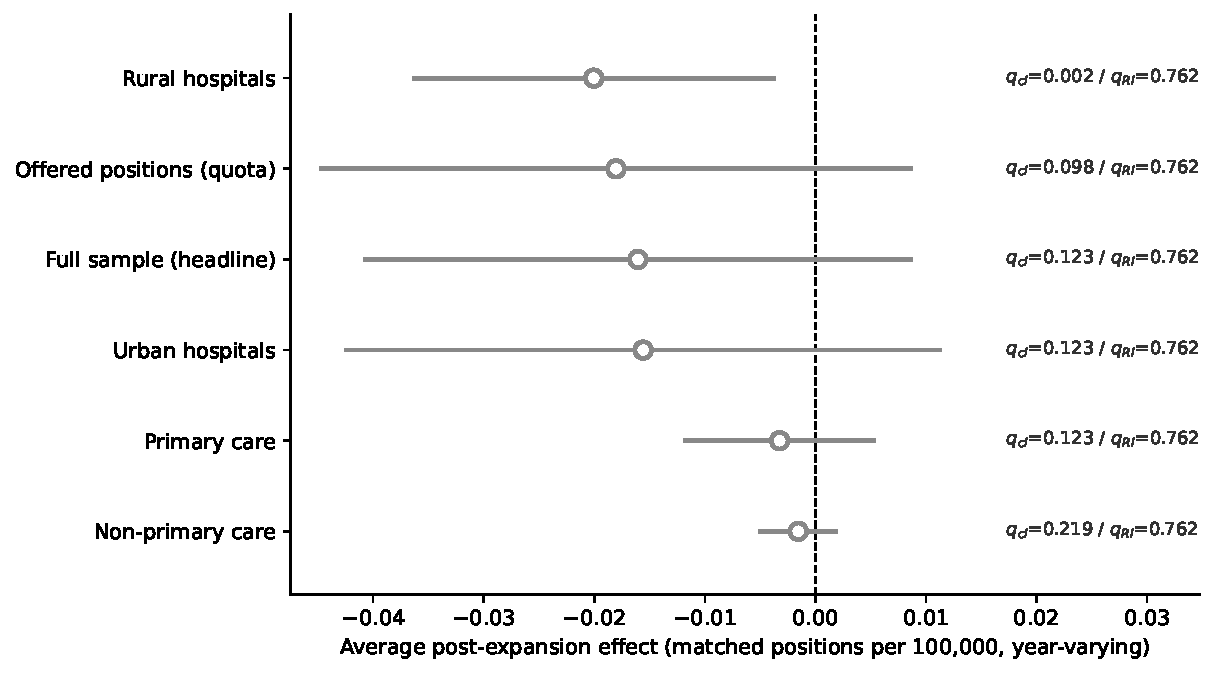
\includegraphics[width=0.85\linewidth]{figures/appx-fdr-forest.pdf}
    \hfill
\caption*{\footnotesize{\textit{Notes:} The figure plots the average post-expansion effect on matched positions per 100{,}000 contemporary (year-varying) population for each member of the primary family of hypotheses, with 95 percent confidence intervals (point estimate $\pm 1.96$ clustered standard errors). The label beside each marker reports the Benjamini--Hochberg false-discovery-rate $q$-value under both inference standards: $q_{cl}$ (clustered) and $q_{RI}$ (randomization inference). Filled markers would denote effects surviving a $5$ percent false-discovery-rate correction under the conservative randomization standard; no member survives it ($q_{RI} \geq 0.76$). Under clustered inference the rural effect is the lone survivor ($q = 0.002$), a result we discount because the rural subsample fails its own pre-trends test (see \cref{subsec:location}). Standard errors are clustered at the state level.}}
\end{figure}

\newpage
\pagebreak

\section{Figures}\label{appendix:figs}

\begin{figure}[H]
    \caption{Effect of Medicaid Expansion on Matched Residency Positions in Levels: Event Study Estimates}
    \label{afig1}
    \centering
      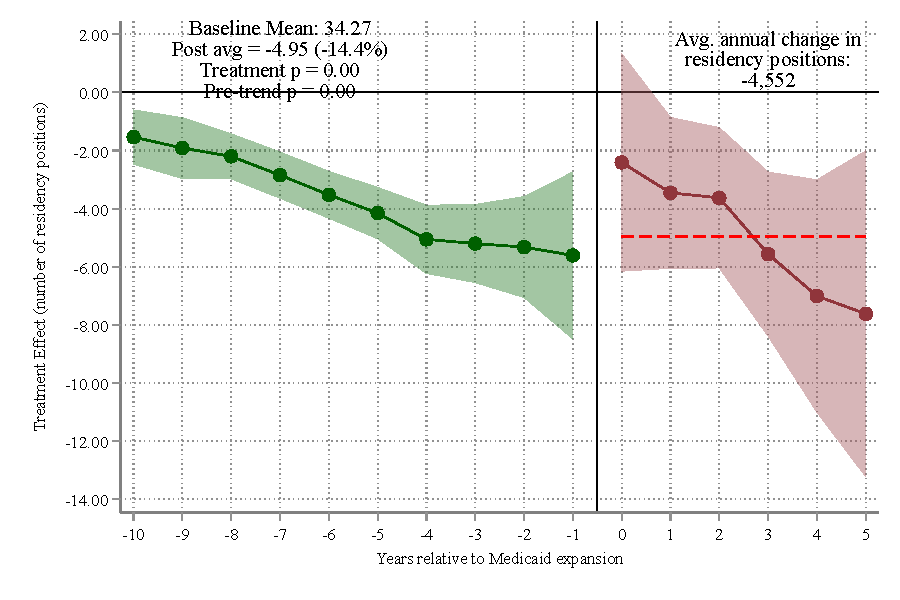
\includegraphics[width=\linewidth]{figures/appx-levels-headline.pdf}
    \hfill
\caption*{\footnotesize{\textit{Notes:} The figure plots event-study coefficients from the imputation estimator of Borusyak, Jaravel, and Spiess (2024), where the outcome is the absolute number of matched residency positions per hospital (not normalized by population). The horizontal axis measures years relative to a state's Medicaid expansion; year 0 is the first year of expansion. Green circles (years $-5$ to $-1$) show pre-expansion coefficients; dark red circles (years $0$ to $+5$) show post-expansion treatment effects. The dashed red line indicates the average post-expansion treatment effect of $-3.85$ positions per hospital, corresponding to a $13.1$ percent decline relative to the pre-expansion mean of $29.43$ matched positions (p $< 0.01$). \textbf{The pre-expansion coefficients in this raw-count specification are large and negative} (on the order of $-2$ positions per hospital, comparable in magnitude to the treatment effect), indicating a violation of parallel trends. This levels estimate therefore corroborates the \emph{direction} of the effect but should not be read as a clean causal magnitude; the paper's primary specification instead normalizes by contemporary population, which restores flat pre-trends (see \cref{subsec:inference}). Shaded bands are 95 percent confidence intervals. Regressions include hospital and year fixed effects. Standard errors are clustered at the state level.}}
\end{figure}

\begin{figure}[H]
    \caption{Effect of Medicaid Expansion on Offered Residency Positions (Quota): Event Study Estimates}
    \label{afig2}
    \centering
      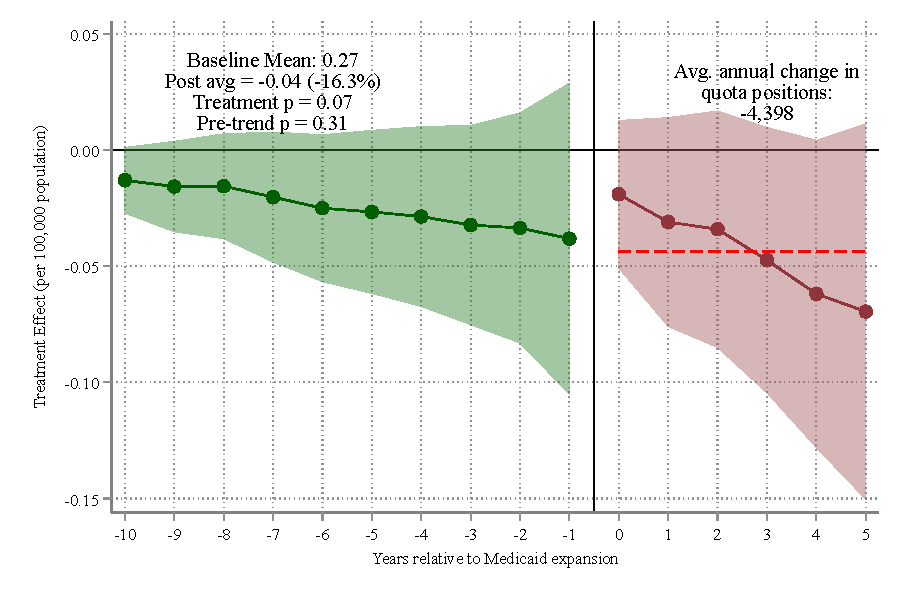
\includegraphics[width=\linewidth]{figures/appx-quota-headline.pdf}
    \hfill
\caption*{\footnotesize{\textit{Notes:} The figure plots event-study coefficients from the imputation estimator of Borusyak, Jaravel, and Spiess (2024), where the outcome is quota positions per 100,000 state population (fixed 2010 population; the year-varying quota estimate of $-0.018$ is reported in the text). Quota positions are the number of positions offered by residency programs in the NRMP Main Residency Match, prior to the matching algorithm; matched positions (the primary outcome in \cref{fig5}) are the subset of offered positions that are ultimately filled. The average post-expansion treatment effect is $-0.03$ ($-13.1$ percent relative to the pre-expansion mean of $0.23$ offered positions per 100,000; p $= 0.01$), corresponding to an average annual reduction of approximately $2{,}771$ offered positions nationally. Shaded bands are 95 percent confidence intervals. Regressions include hospital and year fixed effects. Standard errors are clustered at the state level.}}
\end{figure}

\begin{figure}[H]
    \caption{Effect of Medicaid Expansion on Matched Residency Positions by Hospital Location, in Levels: Event Study Estimates}
    \label{afig3}
    \centering
      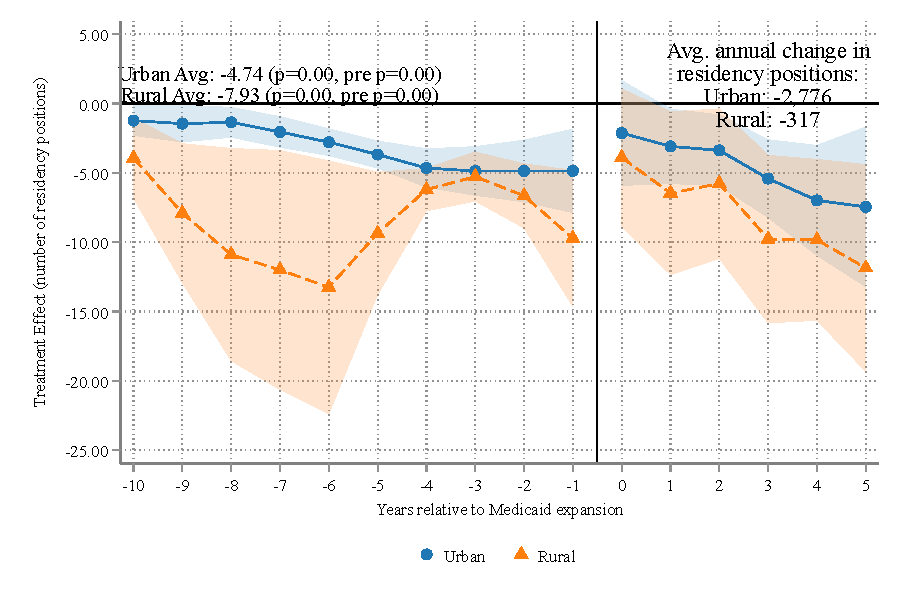
\includegraphics[width=\linewidth]{figures/appx-levels-location.pdf}
    \hfill
\caption*{\footnotesize{\textit{Notes:} The figure plots event-study coefficients from the imputation estimator of Borusyak, Jaravel, and Spiess (2024), estimated in two split-sample regressions for urban (blue circles) and rural (orange triangles) hospitals; each subsample keeps the never-expansion hospitals of its own type as the comparison group, so each series carries its own pre-expansion path and pre-trends test. The outcome is the absolute number of matched residency positions per hospital (not normalized by population). The average post-expansion treatment effect is $-3.62$ positions per hospital for urban hospitals (joint p $< 0.001$; pre-trend p $< 0.001$) and $-8.44$ positions per hospital for rural hospitals (joint p $< 0.001$; pre-trend p $= 0.02$). As with the aggregate levels outcome (\cref{afig1}), both subsamples fail the pre-trends test in levels, so these magnitudes corroborate the direction of the effect only. Translating to aggregate counts, expansion states experienced average annual reductions of approximately $2{,}120$ matched positions at urban hospitals and $338$ at rural hospitals. Shaded bands are 95 percent confidence intervals. Regressions include hospital and year fixed effects and weight by 2010 state population. Standard errors are clustered at the state level.}}
\end{figure}

\begin{figure}[H]
    \caption{Effect of Medicaid Expansion on Offered Residency Positions (Quota) by Hospital Location: Event Study Estimates}
    \label{afig4}
    \centering
      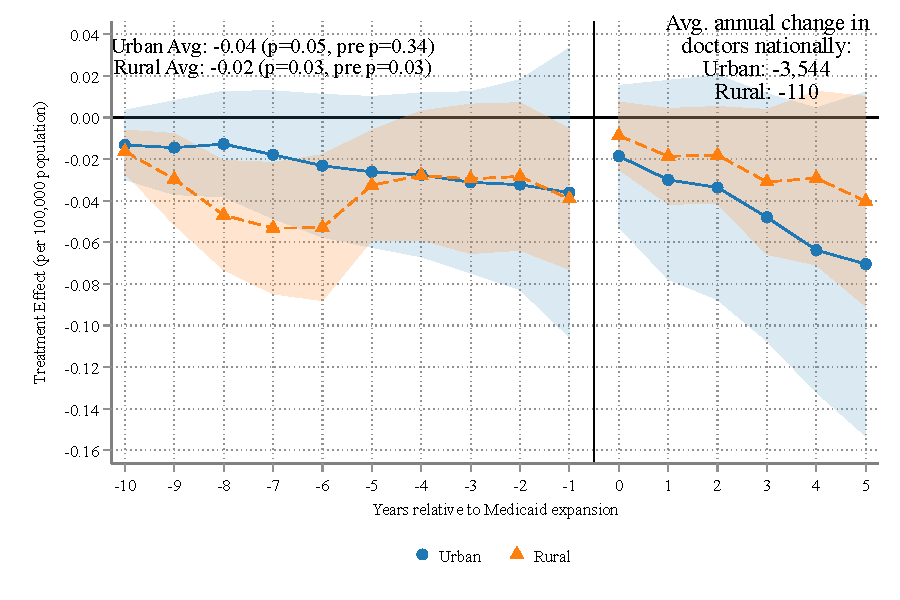
\includegraphics[width=\linewidth]{figures/appx-quota-location.pdf}
    \hfill
\caption*{\footnotesize{\textit{Notes:} The figure plots event-study coefficients from the imputation estimator of Borusyak, Jaravel, and Spiess (2024), estimated in two split-sample regressions for urban (blue circles) and rural (orange triangles) hospitals; each subsample keeps the never-expansion hospitals of its own type as the comparison group, so each series carries its own pre-expansion path and pre-trends test. The outcome is quota positions per 100,000 state population (fixed 2010 population), where quota measures positions offered by programs prior to the matching algorithm. The average post-expansion treatment effect is $-0.031$ for urban hospitals (joint p $= 0.03$; pre-trend p $= 0.10$) and $-0.026$ for rural hospitals (joint p $= 0.03$), similar in magnitude across the two groups. The rural subsample fails its own pre-trends test (p $< 0.001$), so the rural series should be read descriptively. These estimates correspond to average annual reductions of approximately $2{,}452$ offered positions at urban hospitals and $118$ at rural hospitals. Shaded bands are 95 percent confidence intervals. Regressions include hospital and year fixed effects and weight by 2010 state population. Standard errors are clustered at the state level.}}
\end{figure}

\begin{figure}[H]
    \caption{Effect of Medicaid Expansion on Matched Residency Positions by Specialty Type, in Levels: Event Study Estimates}
    \label{afig5}
    \centering
    \begin{subfigure}{\linewidth}
        \centering
        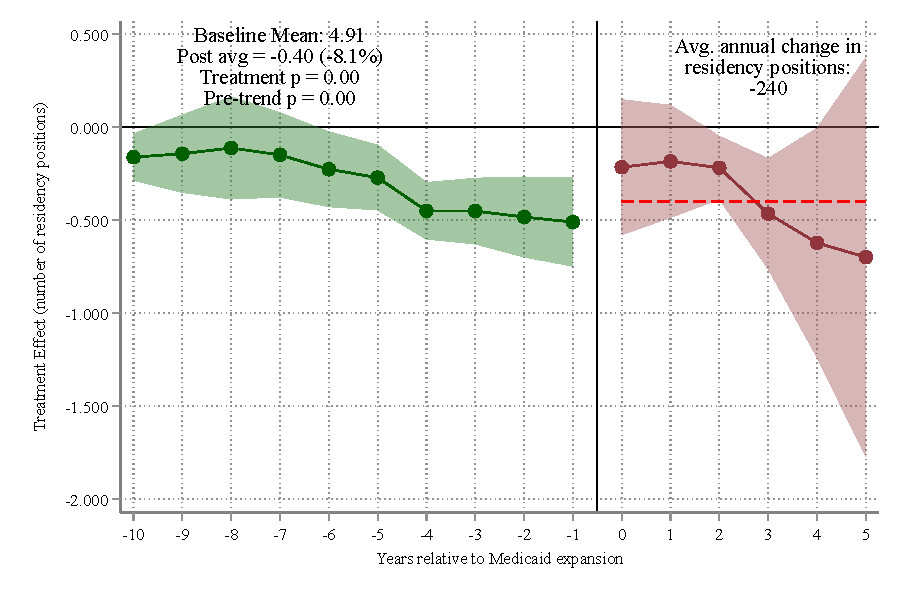
\includegraphics[width=0.75\linewidth]{figures/appx-levels-specialty-nonprimary.pdf}
        \caption{Non-Primary Care Positions}
        \label{afig5:non-prim-care}
    \end{subfigure}
    \hfill
    \begin{subfigure}{\linewidth}
        \centering
        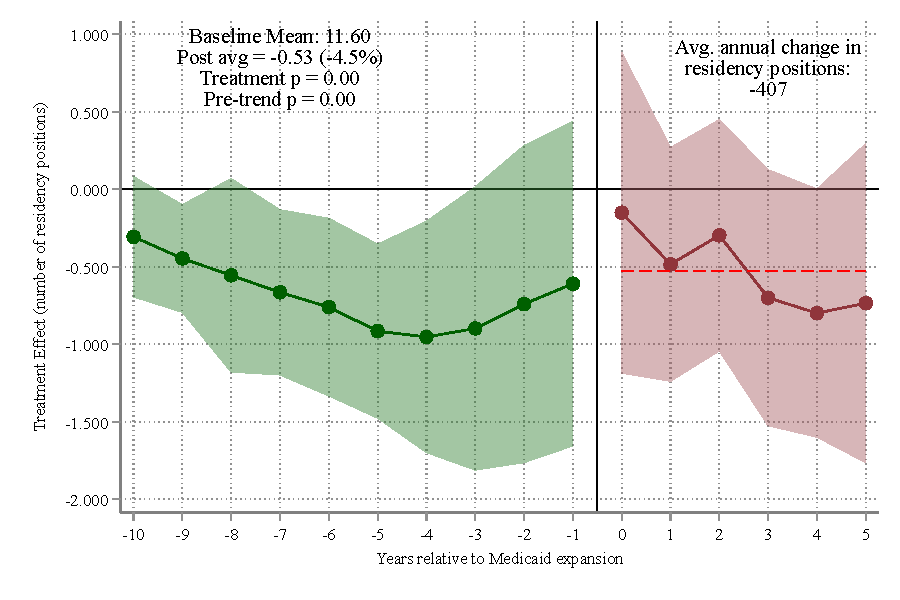
\includegraphics[width=0.75\linewidth]{figures/appx-levels-specialty-primary.pdf}
        \caption{Primary Care Positions}
        \label{afig5:prim-care}
    \end{subfigure}
\caption*{\footnotesize{\textit{Notes:} The figure plots event-study coefficients from the imputation estimator of Borusyak, Jaravel, and Spiess (2024), estimated separately for non-primary care (top panel) and primary care specialties (bottom panel). The outcome is the absolute number of matched residency positions per hospital (not normalized by population). Primary care includes family medicine, internal medicine, and pediatrics. The average post-expansion treatment effect is $-0.37$ positions per hospital for non-primary care ($-8.6$ percent relative to the pre-expansion mean of $4.37$; p $< 0.01$), corresponding to an average annual reduction of approximately $155$ matched positions nationally. For primary care, the average treatment effect is $-0.95$ positions per hospital ($-10.0$ percent relative to the pre-expansion mean of $9.52$; p $< 0.01$), corresponding to an average annual reduction of approximately $562$ positions. Shaded bands are 95 percent confidence intervals. Regressions include hospital and year fixed effects. Standard errors are clustered at the state level.}}
\end{figure}

\begin{figure}[H]
    \caption{Effect of Medicaid Expansion on Offered Residency Positions (Quota) by Specialty Type: Event Study Estimates}
    \label{afig6}
    \centering
    \begin{subfigure}{\linewidth}
        \centering
        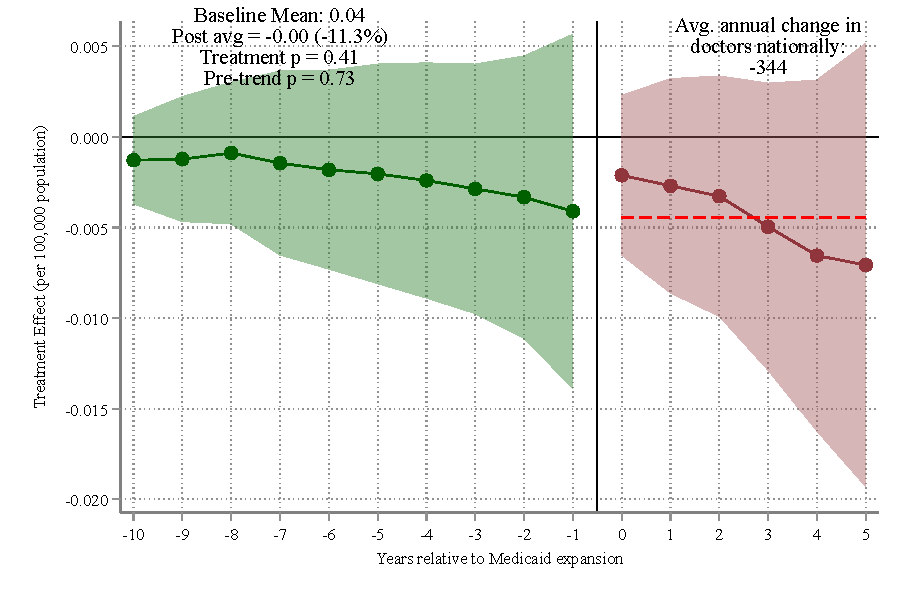
\includegraphics[width=0.75\linewidth]{figures/appx-quota-specialty-nonprimary.pdf}
        \caption{Non-Primary Care Positions}
        \label{afig6:non-prim-care}
    \end{subfigure}
    \hfill
    \begin{subfigure}{\linewidth}
        \centering
        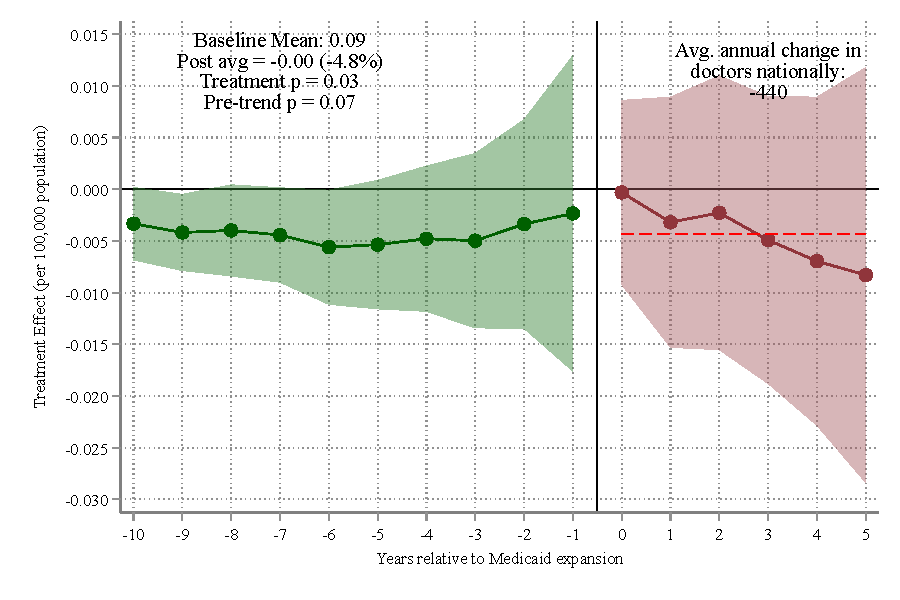
\includegraphics[width=0.75\linewidth]{figures/appx-quota-specialty-primary.pdf}
        \caption{Primary Care Positions}
        \label{afig6:prim-care}
    \end{subfigure}
\caption*{\footnotesize{\textit{Notes:} The figure plots event-study coefficients from the imputation estimator of Borusyak, Jaravel, and Spiess (2024), estimated separately for non-primary care (top panel) and primary care specialties (bottom panel). The outcome is quota positions per 100,000 state population, where quota measures positions offered by programs prior to the matching algorithm. For non-primary care, the average post-expansion treatment effect is $-0.00$ ($-9.7$ percent relative to the pre-expansion mean of $0.04$; p $= 0.12$), corresponding to an average annual reduction of approximately $193$ offered positions nationally. For primary care, the average treatment effect is $-0.01$ ($-9.3$ percent relative to the pre-expansion mean of $0.07$; p $< 0.01$), corresponding to an average annual reduction of approximately $554$ offered positions. Shaded bands are 95 percent confidence intervals. Regressions include hospital and year fixed effects. Standard errors are clustered at the state level.}}
\end{figure}


\begin{figure}[H]
    \caption{Robustness of Event Study Estimates Across Difference-in-Differences Estimators, Total Matched Residency Positions in Levels}
    \label{afig7}
    \centering
      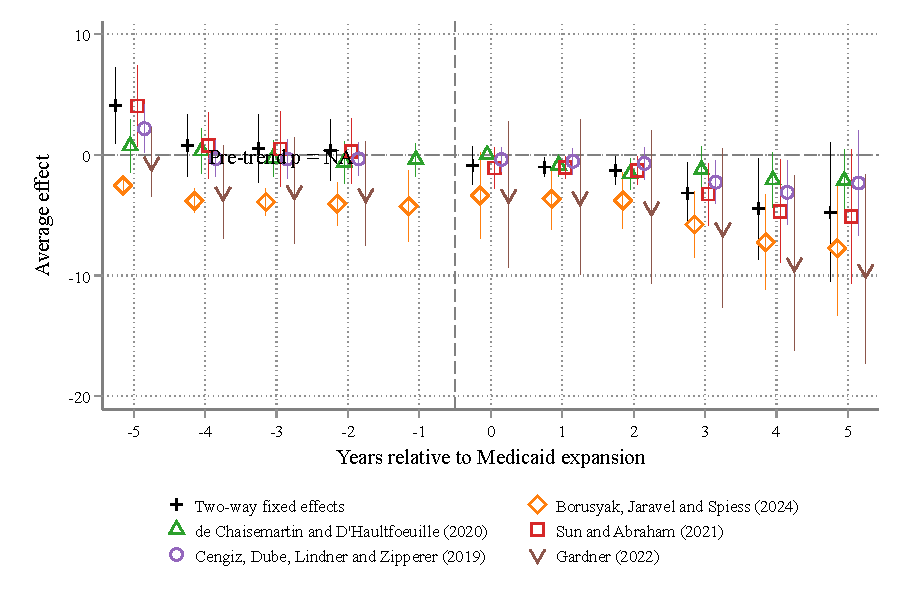
\includegraphics[width=\linewidth]{figures/appx-estimators-levels.pdf}
    \hfill
\caption*{\footnotesize{\textit{Notes:} The figure compares event-study estimates of the effect of Medicaid expansion on the absolute number of matched residency positions per hospital across six difference-in-differences estimators that are robust to treatment-effect heterogeneity under staggered adoption: two-way fixed effects; Borusyak, Jaravel, and Spiess (2024); de Chaisemartin and D'Haultfoeuille (2020); Sun and Abraham (2021); Cengiz, Dube, Lindner, and Zipperer (2019); and Gardner (2022). The heterogeneity-robust estimator of Callaway and Sant'Anna (2021) is excluded because it is not well identified in the sparsely populated never-treated cells of this sample. The pre-trend $p$-value reported in the panel is from the Borusyak, Jaravel, and Spiess (2024) estimator. The dashed vertical line marks the expansion year. Regressions include hospital and year fixed effects. Standard errors are clustered at the state level.}}
\end{figure}

\begin{figure}[H]
    \caption{Robustness of Event Study Estimates Across Difference-in-Differences Estimators, Residency Quota Positions per 100,000 Population}
    \label{afig8}
    \centering
      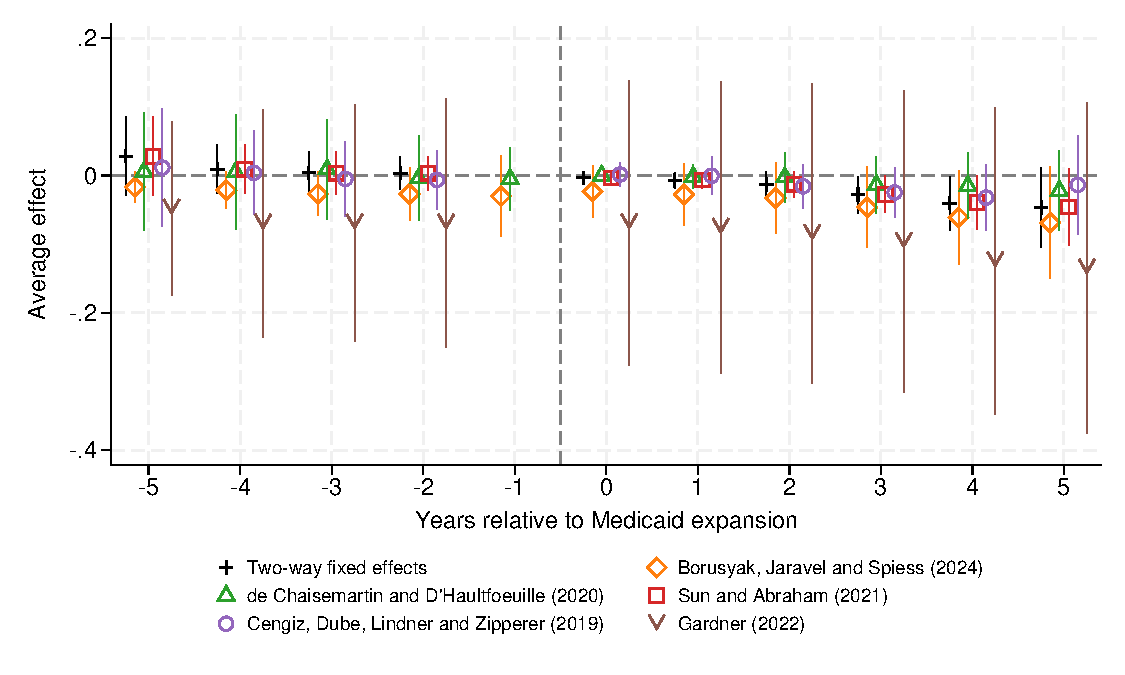
\includegraphics[width=\linewidth]{figures/appx-estimators-quota.pdf}
    \hfill
\caption*{\footnotesize{\textit{Notes:} The figure compares event-study estimates of the effect of Medicaid expansion on quota positions per 100,000 state population across six difference-in-differences estimators. Quota positions measure positions offered by residency programs prior to the matching algorithm. The estimators are: two-way fixed effects; Borusyak, Jaravel, and Spiess (2024); de Chaisemartin and D'Haultfoeuille (2020); Sun and Abraham (2021); Cengiz, Dube, Lindner, and Zipperer (2019); and Gardner (2022); the Callaway and Sant'Anna (2021) estimator is excluded as in the previous figure. The dashed vertical line marks the expansion year. Regressions include hospital and year fixed effects. Standard errors are clustered at the state level.}}
\end{figure}

\begin{figure}[H]
    \caption{Effect of Medicaid Expansion on Matched Residency Positions (Unweighted): Event Study Estimates}
    \label{afig10}
    \centering
      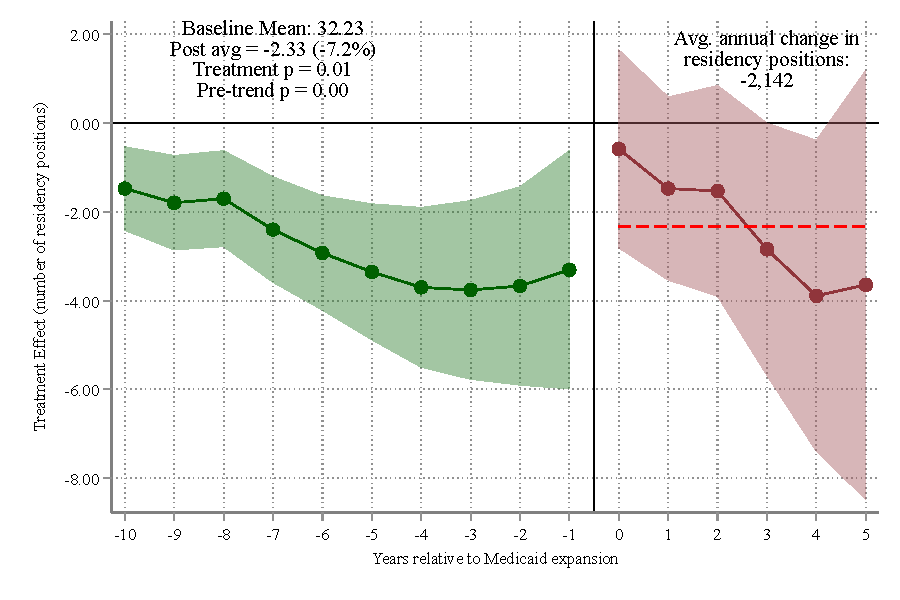
\includegraphics[width=\linewidth]{figures/appx-popcount-levels.pdf}
    \hfill
\caption*{\footnotesize{\textit{Notes:} The figure plots event-study coefficients from the imputation estimator of Borusyak, Jaravel, and Spiess (2024), where the outcome is the number of matched residency positions. This specification is estimated without population weights and includes 2010 state population as a control. The horizontal axis measures years relative to a state's Medicaid expansion; year 0 is the first year of expansion. Green circles (years $-5$ to $-1$) show pre-expansion coefficients. Dark red circles (years $0$ to $+5$) show post-expansion treatment effects. The dashed red line indicates the average post-expansion treatment effect ($-2.49$), which corresponds to approximately $-8.5$ percent relative to the pre-expansion mean of $29.42$ matched positions (p-value $= 0.00$). Translating to aggregate counts, expansion states experienced an average annual reduction of approximately $1{,}610$ matched residency positions relative to the counterfactual. Shaded bands are 95 percent confidence intervals. Regressions include hospital and year fixed effects. Standard errors are clustered at the state level.}}
\end{figure}

\begin{figure}[H]
    \caption{Effect of Medicaid Expansion on Matched Residency Positions per 100,000 Population (Unweighted): Event Study Estimates}
    \label{afig11}
    \centering
      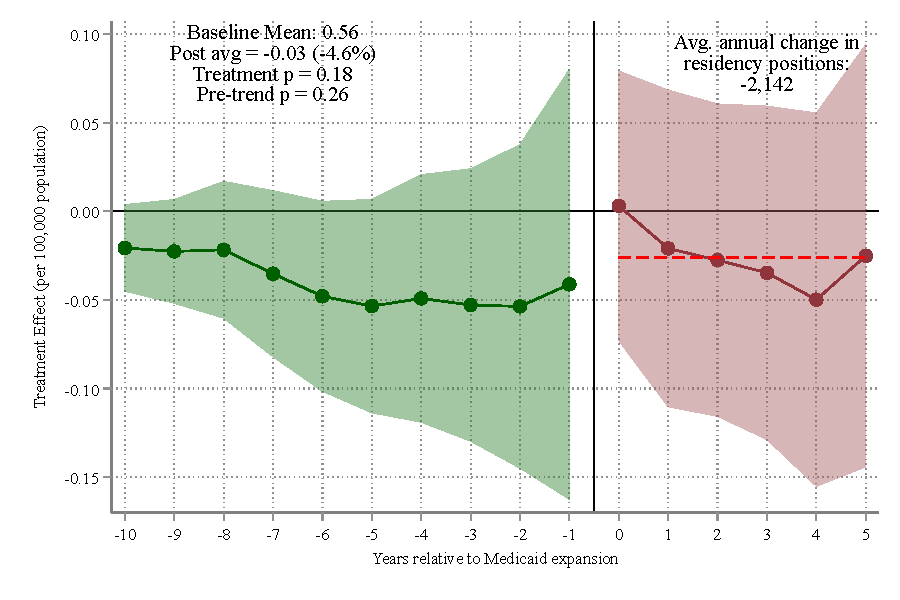
\includegraphics[width=\linewidth]{figures/appx-popcount-percapita.pdf}
    \hfill
\caption*{\footnotesize{\textit{Notes:} The figure plots event-study coefficients from the imputation estimator of Borusyak, Jaravel, and Spiess (2024), where the outcome is matched residency positions per 100,000 state population. This specification is estimated without population weights and includes 2010 state population as a control. The horizontal axis measures years relative to a state's Medicaid expansion; year 0 is the first year of expansion. Green circles (years $-5$ to $-1$) show pre-expansion coefficients. Dark red circles (years $0$ to $+5$) show post-expansion treatment effects. The dashed red line indicates the average post-expansion treatment effect ($-0.02$), which corresponds to approximately $-3.7$ percent relative to the pre-expansion mean of $0.51$ matched positions per 100,000 (p-value $= 0.34$). Translating to aggregate counts, expansion states experienced an average annual reduction of approximately $1{,}610$ matched residency positions relative to the counterfactual. Shaded bands are 95 percent confidence intervals. Regressions include hospital and year fixed effects. Standard errors are clustered at the state level.}}
\end{figure}

\begin{figure}[H]
    \caption{Effect of Medicaid Expansion on Residency Quota Positions per 100,000 Population (Unweighted): Event Study Estimates}
    \label{afig12}
    \centering
      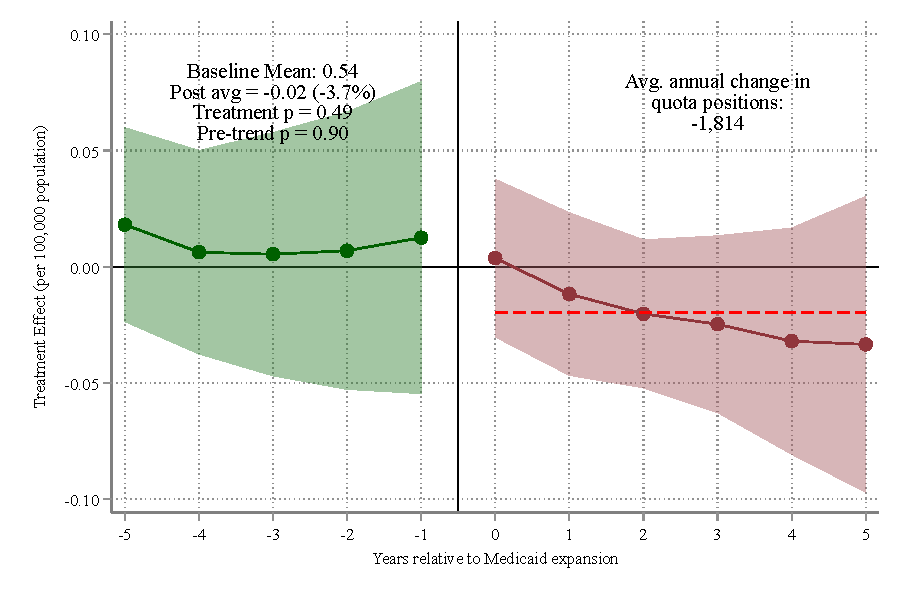
\includegraphics[width=\linewidth]{figures/appx-popcount-quota.pdf}
    \hfill
\caption*{\footnotesize{\textit{Notes:} The figure plots event-study coefficients from the imputation estimator of Borusyak, Jaravel, and Spiess (2024), where the outcome is residency quota (offered) positions per 100,000 state population. This specification is estimated without population weights and includes 2010 state population as a control. The horizontal axis measures years relative to a state's Medicaid expansion; year 0 is the first year of expansion. Green circles (years $-5$ to $-1$) show pre-expansion coefficients. Dark red circles (years $0$ to $+5$) show post-expansion treatment effects. The dashed red line indicates the average post-expansion treatment effect ($-0.02$), which corresponds to approximately $-3.7$ percent relative to the pre-expansion mean of $0.54$ quota positions per 100,000 (p-value $= 0.49$). Translating to aggregate counts, expansion states experienced an average annual reduction of approximately $1{,}814$ quota residency positions relative to the counterfactual. Shaded bands are 95 percent confidence intervals. Regressions include hospital and year fixed effects. Standard errors are clustered at the state level.}}
\end{figure}

\begin{figure}[H]
    \caption{Group-Specific Payment Evidence: Effect of Medicaid Expansion on Direct GME (DGME) Payments by State Medicaid GME Formula}
    \label{afig:fs_dgme}
    \centering
    \begin{subfigure}{\linewidth}
        \centering
        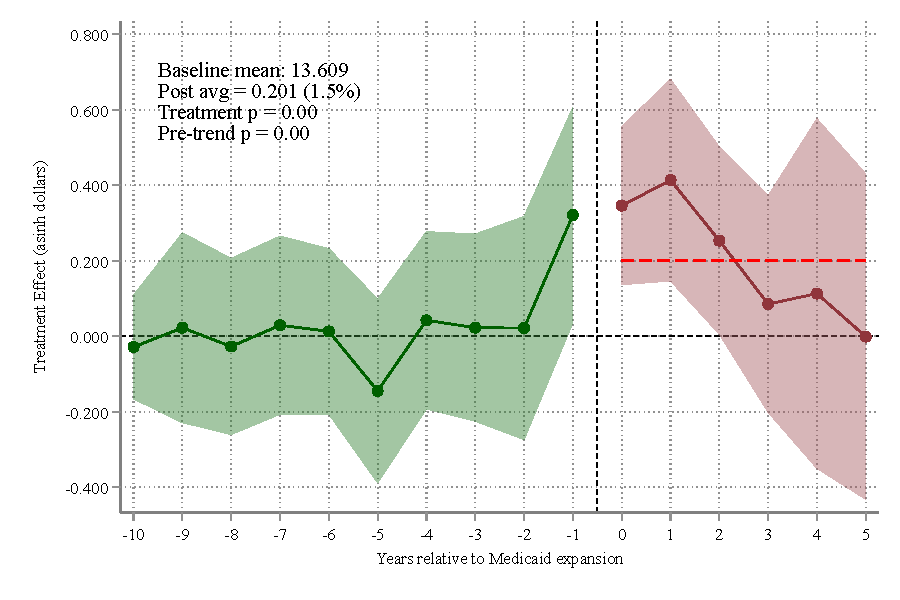
\includegraphics[width=0.75\linewidth]{figures/appx-firststage-dgme-volume.pdf}
        \caption{Volume-Responsive GME States}
        \label{afig:fs_dgme:vol}
    \end{subfigure}
    \hfill
    \begin{subfigure}{\linewidth}
        \centering
        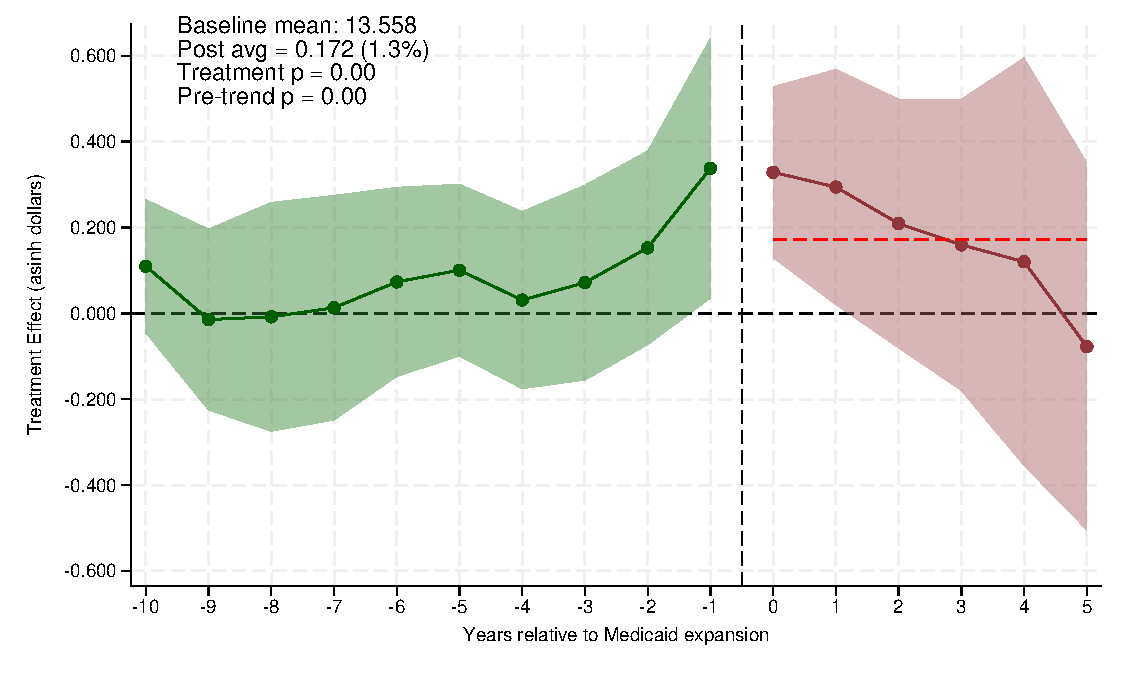
\includegraphics[width=0.75\linewidth]{figures/appx-firststage-dgme-nonresp.pdf}
        \caption{Non-Responsive GME States (Fixed/None)}
        \label{afig:fs_dgme:nonresp}
    \end{subfigure}
\caption*{\footnotesize{\textit{Notes:} The figure re-estimates the Direct GME (DGME) payment event study from \cref{afig13} separately for volume-responsive (top) and non-responsive (bottom) expansion states, each using never-expansion states as the comparison group. The outcome is Medicare cost-report payments, which we read as a proxy for training-related revenue rather than a direct measure of state Medicaid GME payments (see \cref{subsec:mechanisms}). The outcome is the inverse hyperbolic sine (asinh) of DGME payments per teaching hospital, so coefficients approximate proportional changes. In volume-responsive states the average post-expansion effect is $0.24$ (s.e.\ $0.14$; roughly a $24$ percent increase; joint $p < 0.01$), but this panel fails its pre-trend test (pre-trend $p = 0.0002$), so its level should be read with caution; in non-responsive states the effect is $0.10$ (s.e.\ $0.12$; roughly $10$ percent; joint $p < 0.01$; pre-trend $p = 0.30$), less than half as large, though the cross-group difference is imprecise ($0.14$, s.e.\ $0.10$, $p = 0.15$ from a pooled interacted model); see \cref{afig:fs_ftes,afig:fs_perfte} for the FTE/rate decomposition, where the cross-group contrast is sharper. Green circles (years $-5$ to $-1$) show pre-expansion coefficients; dark red circles (years $0$ to $+5$) show post-expansion effects; the dashed red line marks the average post-expansion effect. Shaded bands are 95 percent confidence intervals. Estimates come from CMS Medicare hospital cost reports at the hospital--fiscal-year level. Regressions include hospital and year fixed effects and are unweighted. Standard errors are clustered at the state level.}}
\end{figure}

\begin{figure}[H]
    \caption{Group-Specific Payment Evidence: Effect of Medicaid Expansion on Indirect Medical Education (IME) Payments by State Medicaid GME Formula}
    \label{afig:fs_ime}
    \centering
    \begin{subfigure}{\linewidth}
        \centering
        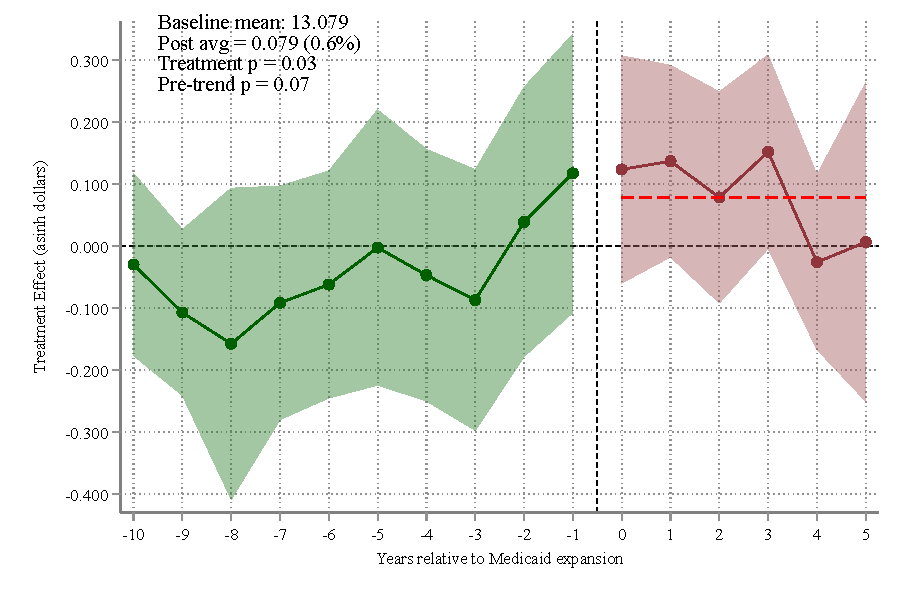
\includegraphics[width=0.75\linewidth]{figures/appx-firststage-ime-volume.pdf}
        \caption{Volume-Responsive GME States}
        \label{afig:fs_ime:vol}
    \end{subfigure}
    \hfill
    \begin{subfigure}{\linewidth}
        \centering
        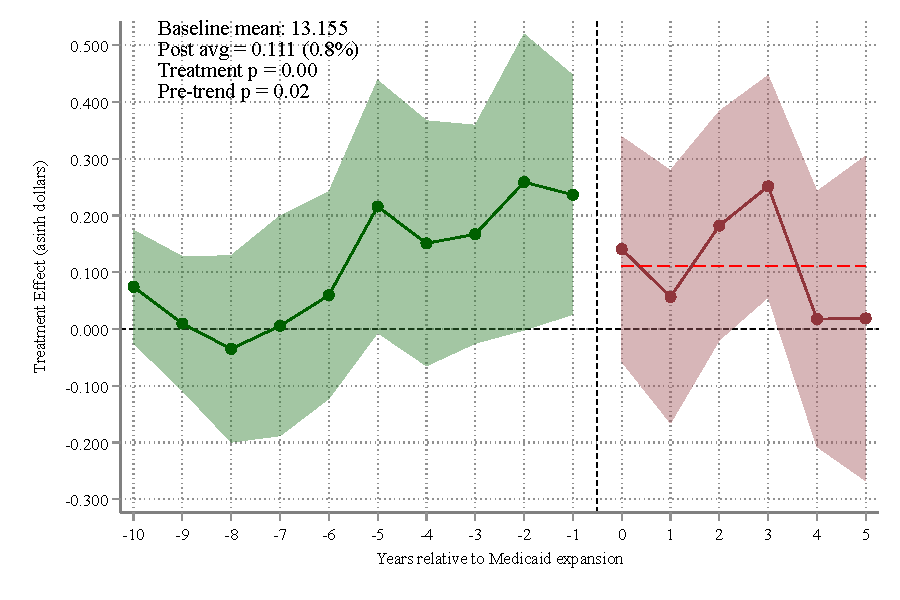
\includegraphics[width=0.75\linewidth]{figures/appx-firststage-ime-nonresp.pdf}
        \caption{Non-Responsive GME States (Fixed/None)}
        \label{afig:fs_ime:nonresp}
    \end{subfigure}
\caption*{\footnotesize{\textit{Notes:} The figure re-estimates the Indirect Medical Education (IME) payment event study from \cref{afig14} separately for volume-responsive (top) and non-responsive (bottom) expansion states, each using never-expansion states as the comparison group. The outcome is the inverse hyperbolic sine (asinh) of IME payments per teaching hospital, from Medicare cost reports (a proxy for training-related revenue; see \cref{subsec:mechanisms}). In volume-responsive states the average post-expansion effect is $0.17$ (s.e.\ $0.08$; roughly a $17$ percent increase; joint $p < 0.01$; pre-trend $p = 0.41$); in non-responsive states it is economically zero and statistically insignificant ($-0.003$, s.e.\ $0.07$; joint $p = 0.30$; pre-trend $p = 0.25$); the cross-group difference is significant ($0.15$, s.e.\ $0.05$, $p = 0.001$ from a pooled interacted model). The differential training-specific revenue gain from expansion is thus concentrated in the volume-responsive states, where residency positions do not contract. Green circles (years $-5$ to $-1$) show pre-expansion coefficients; dark red circles (years $0$ to $+5$) show post-expansion effects. Shaded bands are 95 percent confidence intervals. Regressions include hospital and year fixed effects and are unweighted. Standard errors are clustered at the state level.}}
\end{figure}

\begin{figure}[H]
    \caption{Decomposition of the DGME Payment Response: Resident FTEs by State Medicaid GME Formula}
    \label{afig:fs_ftes}
    \centering
    \begin{subfigure}{\linewidth}
        \centering
        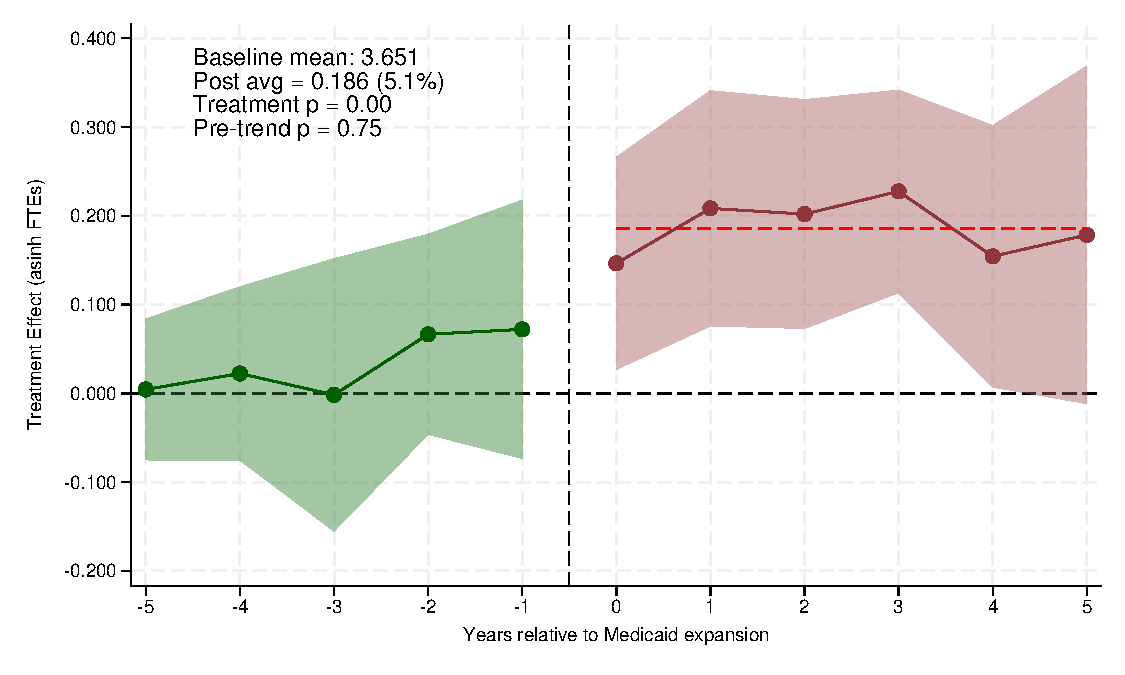
\includegraphics[width=0.75\linewidth]{figures/appx-firststage-dgmeftes-volume.pdf}
        \caption{Volume-Responsive GME States}
    \end{subfigure}
    \hfill
    \begin{subfigure}{\linewidth}
        \centering
        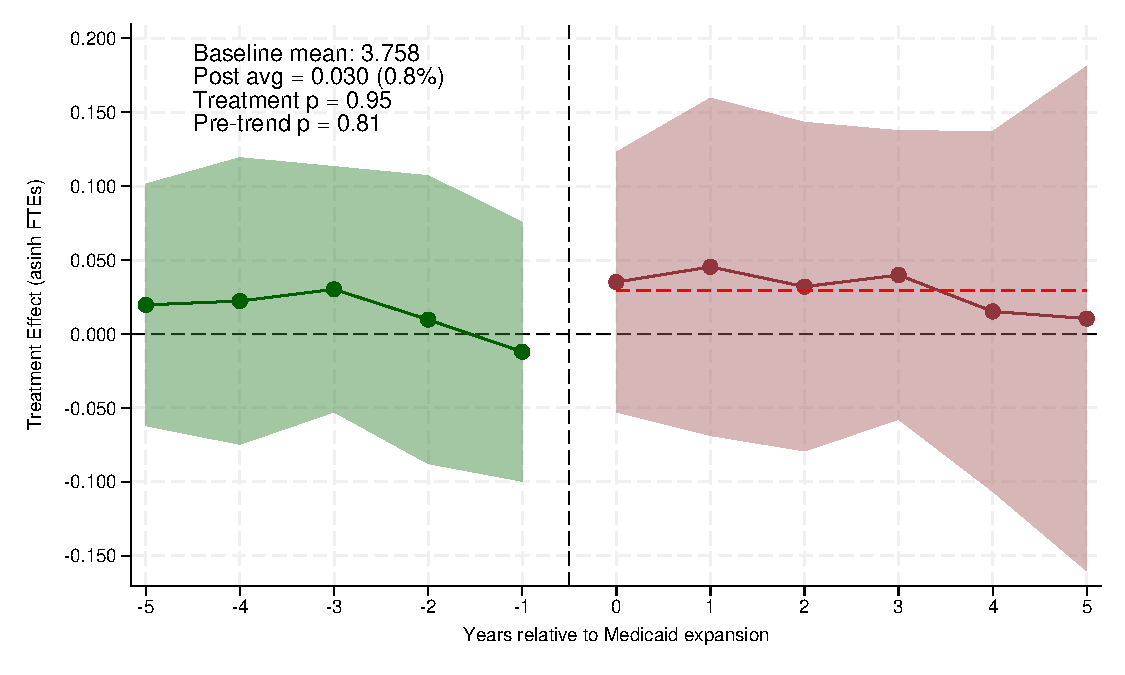
\includegraphics[width=0.75\linewidth]{figures/appx-firststage-dgmeftes-nonresp.pdf}
        \caption{Non-Responsive GME States (Fixed/None)}
    \end{subfigure}
\caption*{\footnotesize{\textit{Notes:} The figure decomposes the Direct GME payment response in \cref{afig:fs_dgme}: the outcome is the inverse hyperbolic sine of cost-report DGME resident FTEs per teaching hospital, so coefficients approximate proportional changes in the number of residents hospitals report for payment purposes. In volume-responsive states resident FTEs rise by roughly $19$ percent (average post effect $0.186$, s.e.\ $0.065$; joint $p < 0.001$) after flat pre-trends ($p = 0.75$); in non-responsive states FTEs do not move ($+3$ percent, s.e.\ $0.055$; joint $p = 0.95$; pre-trend $p = 0.81$). The cross-group difference is $0.14$ (s.e.\ $0.05$, $p = 0.005$ from a pooled interacted model). These estimates are on the full unweighted cost-report sample; on the linked NRMP--cost-report sample with the headline's weights and year convention the FTE response is negative in both arms (see \cref{subsec:inference} and the linked-sample reconciliation exhibits), so the unweighted rise here should not be read as evidence that training expanded. The DGME payment growth in volume-responsive states is therefore a quantity response, while the smaller payment rise in non-responsive states occurs without any growth in residents. Green circles (years $-5$ to $-1$) show pre-expansion coefficients; dark red circles (years $0$ to $+5$) show post-expansion effects. Shaded bands are 95 percent confidence intervals. Estimates come from CMS Medicare hospital cost reports at the hospital--fiscal-year level with never-expansion states as the comparison group. Regressions include hospital and year fixed effects and are unweighted. Standard errors are clustered at the state level.}}
\end{figure}

\begin{figure}[H]
    \caption{Decomposition of the DGME Payment Response: Payment per Resident FTE by State Medicaid GME Formula}
    \label{afig:fs_perfte}
    \centering
    \begin{subfigure}{\linewidth}
        \centering
        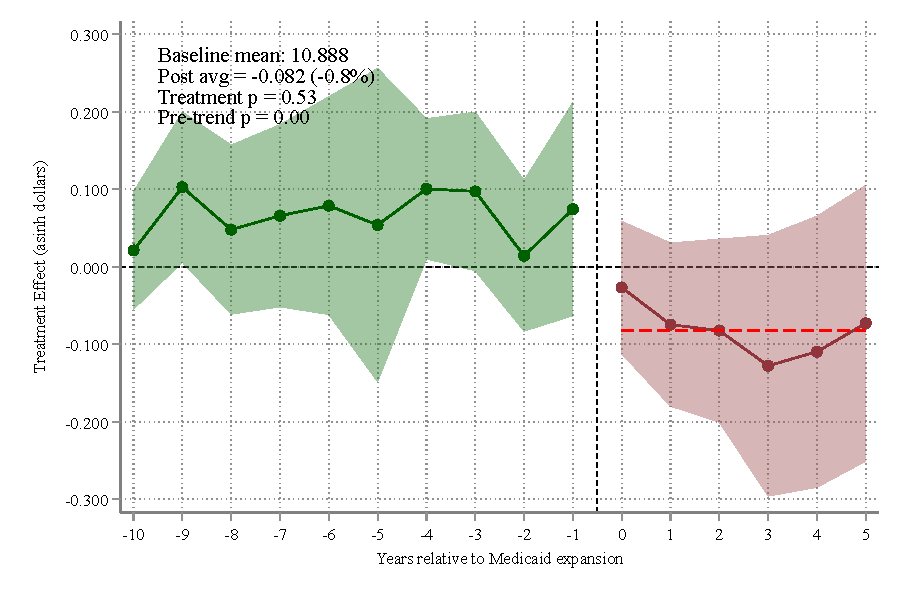
\includegraphics[width=0.75\linewidth]{figures/appx-firststage-dgmeperfte-volume.pdf}
        \caption{Volume-Responsive GME States}
    \end{subfigure}
    \hfill
    \begin{subfigure}{\linewidth}
        \centering
        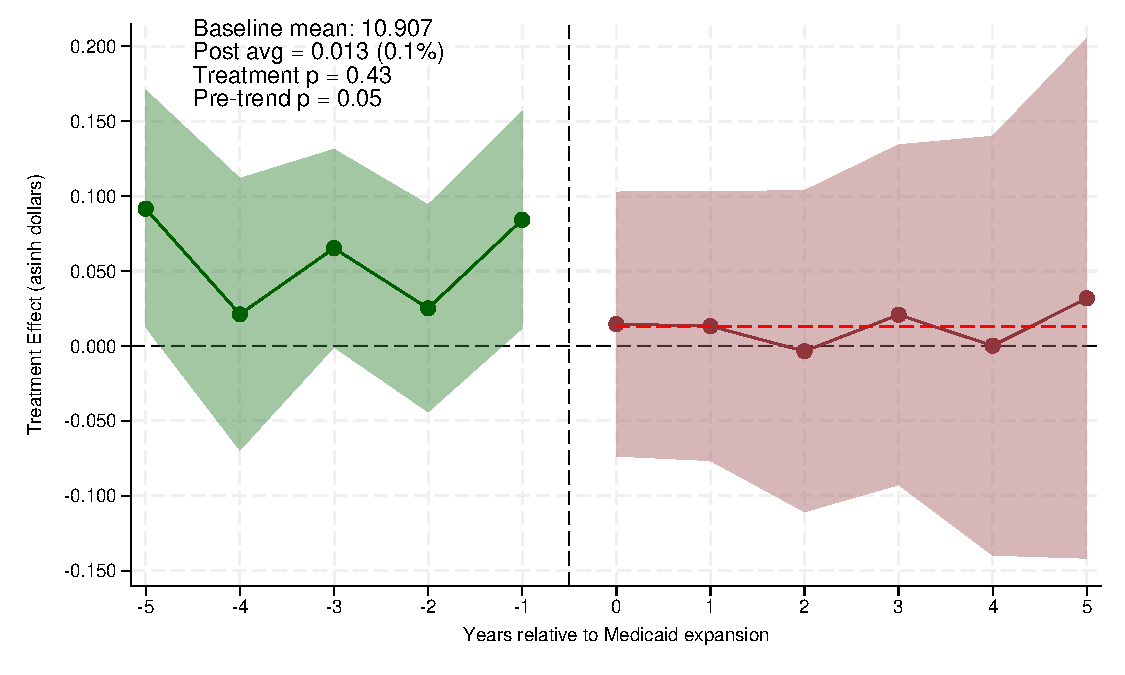
\includegraphics[width=0.75\linewidth]{figures/appx-firststage-dgmeperfte-nonresp.pdf}
        \caption{Non-Responsive GME States (Fixed/None)}
    \end{subfigure}
\caption*{\footnotesize{\textit{Notes:} The figure completes the decomposition in \cref{afig:fs_ftes}: the outcome is the inverse hyperbolic sine of DGME payment per resident FTE (hospitals with positive FTEs only). Per-FTE payments do not rise in either group: the average post effect is $-0.08$ in volume-responsive states (s.e.\ $0.06$; joint $p = 0.53$) and $+0.01$ in non-responsive states (s.e.\ $0.05$; joint $p = 0.43$; pre-trend $p = 0.053$); the cross-group difference is $-0.09$ (s.e.\ $0.04$, $p = 0.03$). The volume-responsive panel exhibits a differential pre-trend (pre-trend $p < 0.001$), so its level should be read with caution; the substantive conclusion---that the payment response is a quantity response, not a rate response---rests on the FTE panel. Green circles (years $-5$ to $-1$) show pre-expansion coefficients; dark red circles (years $0$ to $+5$) show post-expansion effects. Shaded bands are 95 percent confidence intervals. Estimates come from CMS Medicare hospital cost reports at the hospital--fiscal-year level with never-expansion states as the comparison group. Regressions include hospital and year fixed effects and are unweighted. Standard errors are clustered at the state level.}}
\end{figure}

\begin{figure}[H]
    \caption{Robustness to Not-Yet-Treated Controls: Effect of Medicaid Expansion on Matched Residency Positions per 100,000 Population}
    \label{afig:notyet}
    \centering
      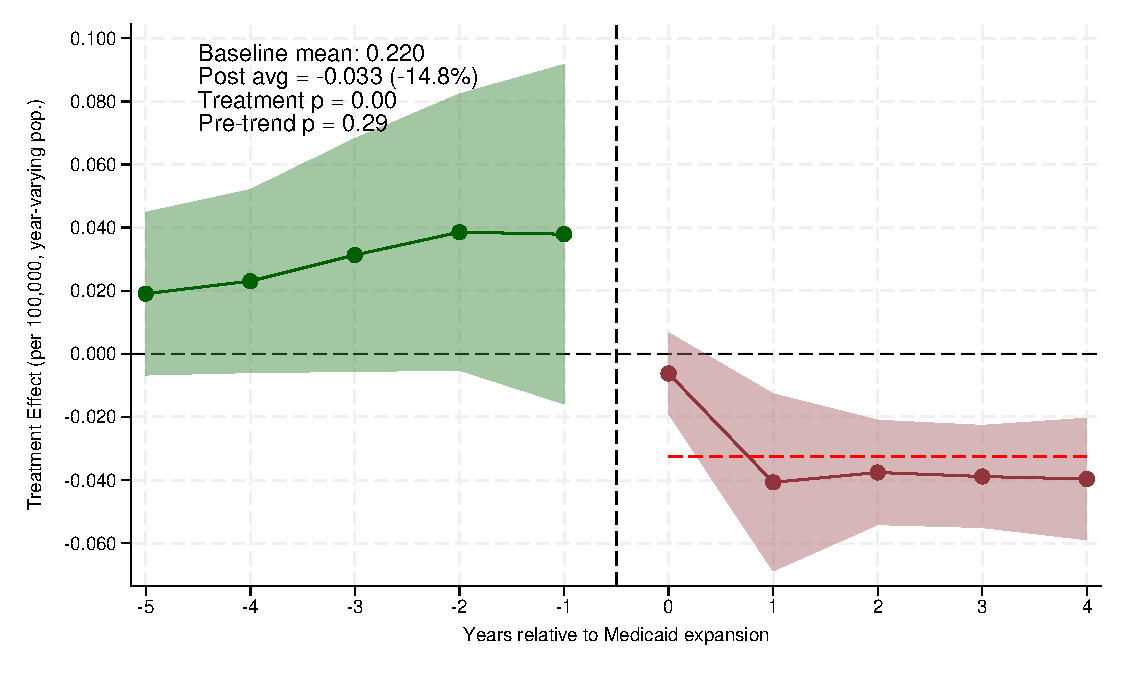
\includegraphics[width=\linewidth]{figures/appx-notyet.pdf}
    \hfill
\caption*{\footnotesize{\textit{Notes:} The figure re-estimates the main event study after dropping never-expansion states, so identification rests solely on variation in the timing of expansion among eventually-treated states (the not-yet-treated design). The outcome is matched positions per 100,000 contemporary (year-varying) population. Because the last-treated cohort has no valid comparison at horizon $+5$ under the not-yet-treated design, the event study is estimated over horizons $0$ to $+4$. The average post-expansion effect is $-0.033$ (a $14.8$ percent decline relative to the pre-expansion mean of $0.22$; joint clustered $p < 0.01$; randomization-inference $p = 0.38$, see \cref{subsec:inference})---larger and, under clustered inference, more precisely estimated than the full-sample effect---with flat pre-expansion coefficients (pre-trend $p = 0.29$). The contraction is therefore not an artifact of the never-expansion comparison group; if anything it is sharper when identification rests solely on the timing of expansion among adopters. Green circles (years $-5$ to $-1$) show pre-expansion coefficients; dark red circles (years $0$ to $+4$) show post-expansion effects; the dashed red line marks the average post-expansion effect. Shaded bands are 95 percent confidence intervals. Regressions include hospital and year fixed effects and weight by 2010 state population. Standard errors are clustered at the state level.}}
\end{figure}

\begin{figure}[H]
    \caption{Balanced-Cohort Event Study: 2014 Adopters Only}
    \label{afig:cohort2014}
    \centering
      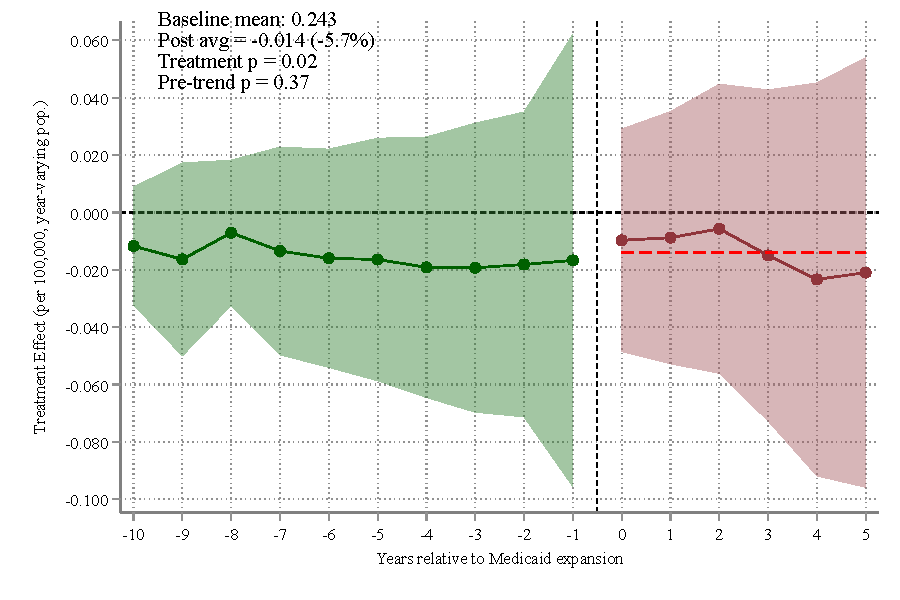
\includegraphics[width=\linewidth]{figures/appx-cohort2014.pdf}
    \hfill
\caption*{\footnotesize{\textit{Notes:} The figure re-estimates the main event study restricting treatment to the 2014 expansion cohort (the largest wave), with never-expansion states as the comparison group, so that every event-time coefficient is identified from the same fixed set of treated states. The outcome is matched positions per 100,000 contemporary (year-varying) population. The average post-expansion effect is $-0.015$ (a $7.5$ percent decline relative to the pre-expansion mean of $0.20$; joint $p = 0.16$ in this smaller single-cohort sample), and the event-time coefficients widen monotonically from $-0.004$ at horizon $0$ to $-0.024$ at horizon $+5$, following flat pre-expansion coefficients (pre-trend $p = 0.97$). Because cohort composition is held fixed, the widening path here reflects genuine dynamics rather than the changing composition of cohorts across horizons. Green circles (years $-5$ to $-1$) show pre-expansion coefficients; dark red circles (years $0$ to $+5$) show post-expansion effects; the dashed red line marks the average post-expansion effect. Shaded bands are 95 percent confidence intervals. Regressions include hospital and year fixed effects and weight by 2010 state population. Standard errors are clustered at the state level.}}
\end{figure}

\begin{figure}[H]
    \caption{Leave-One-State-Out Estimates of the Headline Effect}
    \label{afig:loo}
    \centering
      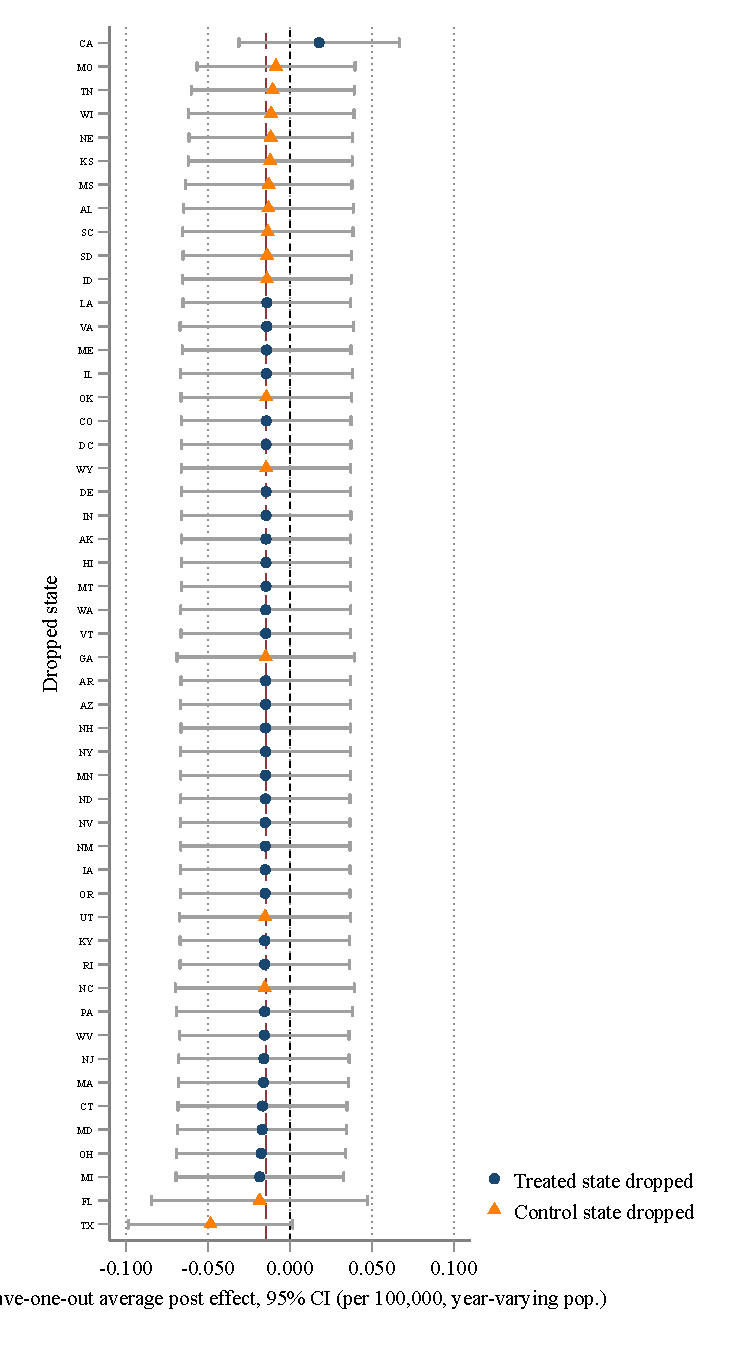
\includegraphics[width=0.8\linewidth]{figures/appx-loo.pdf}
    \hfill
\caption*{\footnotesize{\textit{Notes:} The figure plots the average post-expansion effect on matched positions per 100,000 contemporary (year-varying) population, re-estimated after dropping each treated state in turn (34 estimates, sorted). The dashed maroon line marks the full-sample estimate ($-0.016$); the thin black line marks zero. Every leave-one-out estimate remains negative (range $-0.018$ to $-0.001$), so the sign of the effect does not depend on any single state; dropping California alone, however, shrinks the estimate to $-0.001$, reflecting the concentration of identifying weight documented in \cref{subsec:inference}. Regressions include hospital and year fixed effects and weight by 2010 state population.}}
\end{figure}

\begin{figure}[H]
    \caption{HonestDiD Sensitivity to Violations of Parallel Trends}
    \label{afig:honest}
    \centering
    \begin{subfigure}{0.48\linewidth}
        \centering
        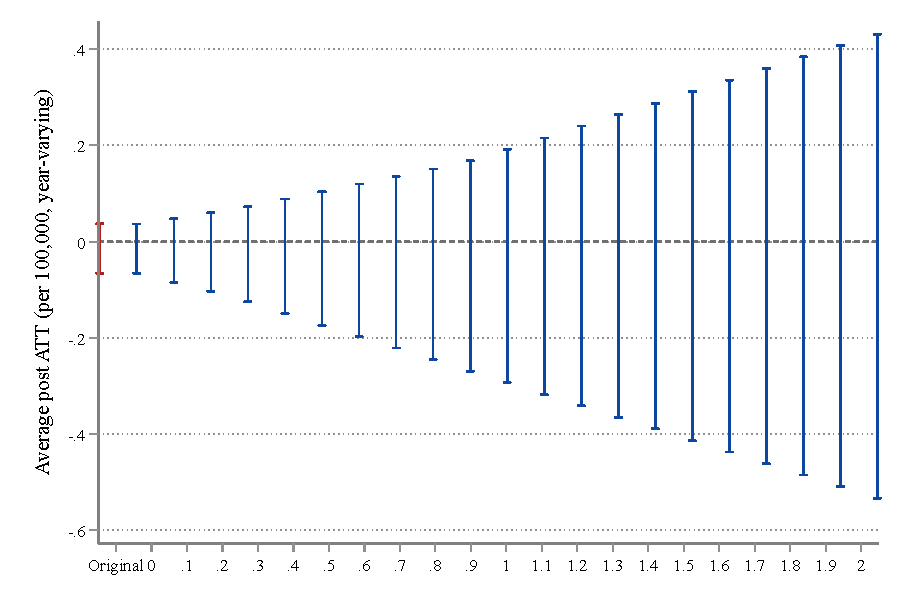
\includegraphics[width=\linewidth]{figures/appx-honestdid-headline.pdf}
        \caption{Headline (per 100,000, year-varying)}
        \label{afig:honest:head}
    \end{subfigure}
    \hfill
    \begin{subfigure}{0.48\linewidth}
        \centering
        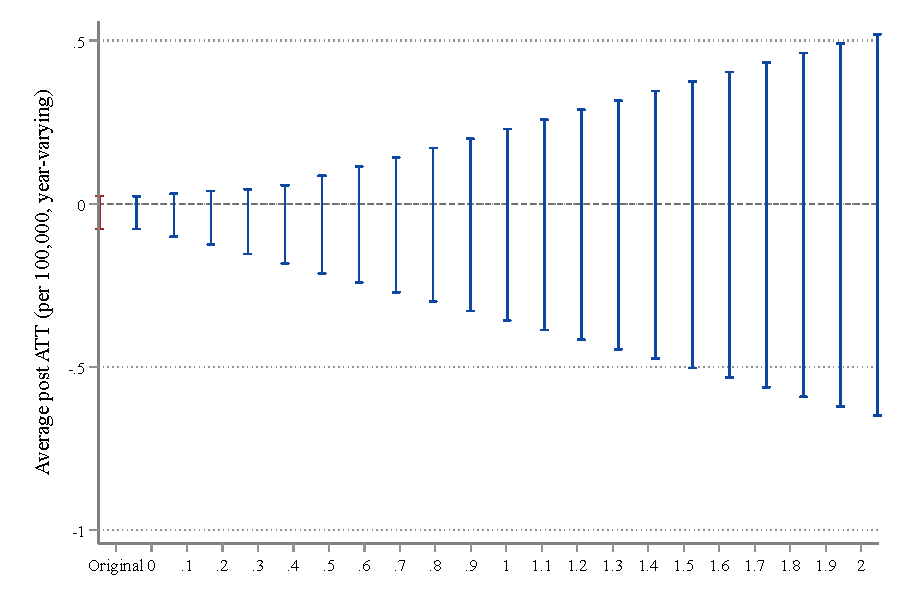
\includegraphics[width=\linewidth]{figures/appx-honestdid-nonresp.pdf}
        \caption{Non-Responsive States}
        \label{afig:honest:nonresp}
    \end{subfigure}
    \begin{subfigure}{0.48\linewidth}
        \centering
        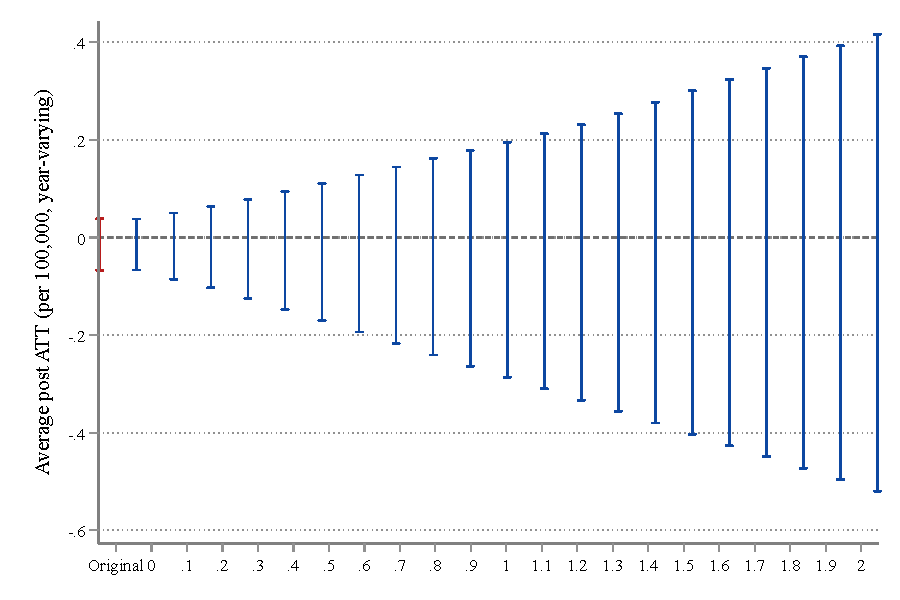
\includegraphics[width=\linewidth]{figures/appx-honestdid-urban.pdf}
        \caption{Urban Hospitals}
        \label{afig:honest:urban}
    \end{subfigure}
\caption*{\footnotesize{\textit{Notes:} The figure reports \textcite{rambachan2023more} sensitivity analysis for the average post-expansion effect on matched positions per 100,000 contemporary population, under the relative-magnitudes restriction $\Delta^{RM}(\bar{M})$, which bounds the post-period differential trend by $\bar{M}$ times the largest pre-period differential trend. Each panel plots the robust 95 percent confidence interval for the average post ATT as $\bar{M}$ increases. For the headline effect, the non-responsive mechanism panel, and the urban subsample, the robust confidence interval includes zero even at $\bar{M} = 0$ (exact parallel trends), confirming that the average magnitude is not distinguishable from zero at conventional levels; what the design supports is the sign and the growing dynamic path of the effect, together with the clustered joint tests and the not-yet-treated estimate. The leftmost interval in each panel is the original CI. Estimates use the Borusyak, Jaravel, and Spiess (2024) event-study coefficients with state-clustered standard errors.}}
\end{figure}

\newpage
\pagebreak


\newpage
\pagebreak

% Appendix Bibliography
\begingroup
\setstretch{1.0}
\setlength\bibitemsep{0pt}
\printbibliography[title=References for Online Appendix]
\endgroup
\pagebreak
\end{refsection}

\end{document}